
\documentclass[
  pagesize=pdftex,
  paper=letter,
  numbers=noenddot,
  captions=tableheading,
  chapterprefix,
  %parskip=half,
  %fontsize=10.5pt,
  fontsize=11pt,
  %twoside,
  BCOR=-12mm,
  DIV=9,
  %headings=openright,
  %toc=chapterentrywithdots,   % not yet supported
  toc=listof,
  toc=bib,
  %draft
]{scrreprt}

\newcommand{\longtitle}{%
Efficient Deep Learning of 3D Structural Brain MRIs for Manifold Learning and
Lesion Segmentation with Application to Multiple Sclerosis}

%\usepackage[margin=3cm]{geometry}
\usepackage{ifthen}

\usepackage{fixltx2e}
% Charater sets, fonts and basics

\usepackage{ifxetex}

\ifxetex

\usepackage{fontspec}
\setsansfont[Scale=1,Mapping=tex-text,BoldFont={Optima-Bold},ItalicFont={Optima-Italic}]{Optima}

\else

\usepackage[latin1]{inputenc}
\usepackage[T1]{fontenc}
%\renewcommand*\sfdefault{uop}

\fi

%\usepackage[sc, osf]{mathpazo}
\usepackage[sc]{mathpazo}
\usepackage[scaled=.9]{luximono}
\linespread{1.10}

\usepackage[english]{babel}
\usepackage[english=british]{csquotes}
\addto\captionsenglish{% Replace "english" with the language you use
  \renewcommand{\contentsname}%
    {Table of Contents}%
}

\usepackage{microtype}
\makeatletter
\def\MT@register@subst@font{\MT@exp@one@n\MT@in@clist\font@name\MT@font@list
   \ifMT@inlist@\else\xdef\MT@font@list{\MT@font@list\font@name,}\fi}
\makeatother 

% Math stuff
%\usepackage{dsfont,amsmath,amssymb,latexsym,soul}
\usepackage{amsmath,mathtools}
\usepackage{amsbsy,dsfont,soul,calc}
\DeclareMathOperator{\sinc}{sinc}
\DeclareMathOperator{\sigm}{sigm}
\DeclareMathOperator{\fft}{fft}
\DeclareMathOperator{\ifft}{ifft}
\sodef\so{}{.14em}{.4em plus.1em minus .1em}{.4em plus.1em minus .1em}

\usepackage[autokw]{svn-multi}
\svnid{$Id: preamble.tex 41 2012-08-01 17:29:41Z tbrosch $}

% Tikz
\usepackage{atbegshi}
\usepackage{tikz}
\usetikzlibrary{intersections,decorations.pathreplacing,fit,calc,positioning,shapes.geometric,matrix}
\tikzstyle{every node}+=[font=\sffamily\small]
\pgfdeclarelayer{background}
\pgfsetlayers{background,main}

%\usetikzlibrary{external}
%\tikzexternalize[prefix=tikzfigures/temp/] % activate
%\tikzset{external/export=false}
\newcommand{\tikzexternal}[2][false]{%
%\tikzset{external/export=true, external/remake next=#1}%
%\tikzsetnextfilename{#2}%
}

% Special Table hacks
\usepackage{array,booktabs,dcolumn,rotating,multirow,etoolbox}

\robustify\bfseries % requires etoolbox
\newcommand{\minitab}[2][l]{\begin{tabular}{#1}#2\end{tabular}}

\newcolumntype{d}[1]{%
>{\DC@{.}{.}{#1}}l<{\DC@end}%
}

\newcolumntype{.}{D{.}{.}{-1}}
\newcolumntype{L}[1]{>{\raggedright\arraybackslash}p{#1}}

%\usepackage[sf,SF]{subfigure}
\usepackage[font={sf,small},labelfont=md,subrefformat=parens]{subfig}

% Units
\usepackage{xfrac}
\usepackage[alsoload=binary]{siunitx}
\sisetup{
  seperr,
  %repeatunits=false,
  product-units = single,
  trapambigerr=false,
  trapambigrange=false,
  %tophrase={{ bis }},
  valuemode=math,
  unitmode=math,
  quotient-mode=fraction,
  fraction-function=\sfrac
}

\usepackage{tocstyle}
\newtocstyle[KOMAlike][leaders]{thesis}{
  %\settocfeature[-1]{dothook}{\bfseries}
  %\settocfeature[0]{dothook}{\bfseries}
}
\usetocstyle{thesis}

% Enumerates
\usepackage{paralist}

\usepackage{varioref}
\usepackage[
	pdfpagemode=UseOutlines,
	pdfdisplaydoctitle=true,
	pdflang=en,
	pagebackref,
	bookmarksopen=true,
	bookmarksopenlevel={1}
]{hyperref}

% % Change Layout of Backref
\renewcommand*{\backref}[1]{%
  % default interface
  % #1: backref list
  %
  % We want to use the alternative interface,
  % therefore the definition is empty here.
}%
\renewcommand*{\backrefalt}[4]{%
  % alternative interface
  % #1: number of distinct back references
  % #2: backref list with distinct entries
  % #3: number of back references including duplicates
  % #4: backref list including duplicates
  \ifnum#1=0%
  \footnotesize\sffamily\color{red!50!gray}(not cited)%
  \else%
  \ifnum#1=1%
  \footnotesize\sffamily\color{gray}(cited on page~#2)%
  \else%
  \footnotesize\sffamily\color{gray}(cited on pages~#2)%
  \fi%
  \fi%
}

% Extraabstand fuer Fussnoten
\setlength{\skip\footins}{2em}

% Handle floats right
%\usepackage[above,below]{placeins}
%\usepackage{placeins}

\usepackage[version=3]{mhchem}

%\bibliographystyle{plain}
\usepackage{bibgerm}
\usepackage[sort]{natbib}
\bibliographystyle{gerapali}
%\bibliographystyle{gerplain}

% Listings
\usepackage{listings}

% Color definition
% Define special colors
\definecolor{listcomment}{rgb}{0.325,0.761,0.259}
\definecolor{listkeyword}{rgb}{0.243,0.306,0.408}
\definecolor{listnumbers}{gray}{0.65}
\definecolor{listlightgray}{gray}{0.955}
\definecolor{shadecolor}{named}{listlightgray}
\definecolor{stringcolor}{rgb}{0.341,0.243,0.416}

% Setup the listings environment
\lstset{
  frame = tb,
  framerule = 0.25pt,
  float,
  backgroundcolor={\color{listlightgray}},
  basicstyle = {\ttfamily\footnotesize},
  keywordstyle = {\ttfamily\color{listkeyword}\textbf},
  identifierstyle = {\ttfamily},
  commentstyle = {\ttfamily\color{listcomment}\textit},
  stringstyle = {\ttfamily\color{stringcolor}},
  showstringspaces = false,
  showtabs = false,
  numbers = left,
  numbersep = 6pt,
  numberstyle={\ttfamily\color{listnumbers}},
  tabsize = 2,
  language=C++,
  floatplacement=tb
  captionpos=b,
  escapeinside={<@}{@>},
  abovecaptionskip=7pt,
  morekeywords={__global__, __host__, __device__, uint, texture, float4, fmatrix4}
}

\usepackage[vlined,linesnumbered]{algorithm2e}
\SetNlSty{}{}{}
\SetArgSty{}
\DontPrintSemicolon

\usepackage[acronym,nonumberlist,toc,nomain]{glossaries}
\renewcommand*{\glspostdescription}{}
\setlength{\glsdescwidth}{0.7\textwidth}
\glossarystyle{super}
\renewcommand*{\glsgroupskip}{}

\AtBeginDocument{\labelformat{lstlisting}{Listing #1}}
\AtBeginDocument{\labelformat{chapter}{Chap\mbox{ter #1}}}
\AtBeginDocument{\labelformat{section}{Sec\mbox{tion #1}}}
\AtBeginDocument{\labelformat{subsection}{Sec\mbox{tion #1}}}
\AtBeginDocument{\labelformat{equation}{(#1)}}
\AtBeginDocument{\labelformat{table}{T\mbox{able #1}}}
\AtBeginDocument{\labelformat{figure}{F\mbox{igure #1}}}
\AtBeginDocument{\labelformat{Definition}{D\mbox{efinition #1}}}
%\AtBeginDocument{\labelformat{Satz}{Satz~#1}}
%\AtBeginDocument{\labelformat{Beispiel}{Beispiel~#1}}
%\AtBeginDocument{\labelformat{Beweis}{Beweis~#1}}

% Headings and footer
\usepackage{scrpage2}
\pagestyle{scrheadings}
\clearscrheadfoot
\ohead{\headmark}
\ofoot[\pagemark]{\pagemark}

\setheadsepline{.4pt}
\addtokomafont{pageheadfoot}{\normalfont\sffamily\small}
\addtokomafont{caption}{\sffamily\small}
\addtokomafont{captionlabel}{\sffamily\bfseries\small}
\addtokomafont{pagefoot}{\normalsize}
%\addtokomafont{chapter}{\glsresetall}
%\addtokomafont{page}{\normalsize}
%\automark[subsection]{section}
\automark{chapter}

%\addtokomafont{section}{
%{\tikzset{external/export=false}\tikz \fill[left color=blue!50,right
%color=white] (0,0) rectangle (\textwidth,1pt);}\\*%
%}
\addtokomafont{dictumtext}{\normalfont\itshape}
\addtokomafont{dictumauthor}{\normalfont}

\usepackage[textwidth=3.3cm, textsize=footnotesize,
colorinlistoftodos, shadow]{todonotes}
\usepackage{textcomp,xspace}
\usepackage{dsfont,amsmath,amssymb,amsbsy}
\usepackage{setspace,comment}

\newcommand{\vect}[1]{\mathbf{#1}}
\newcommand{\R}{\ensuremath{\mathds{R}}}
\newcommand{\Q}{\ensuremath{\mathds{Q}}}
\newcommand{\N}{\ensuremath{\mathds{N}}}
\newcommand{\I}{\ensuremath{\mathds{I}}}
\newcommand{\E}{\ensuremath{\mathds{E}}}
\newcommand{\Z}{\ensuremath{\mathds{Z}}}
\newcommand{\D}{\ensuremath{\mathds{D}}}
\newcommand{\W}{\ensuremath{\mathds{W}}}
%\newcommand{\B}{\ensuremath{\mathds{B}}}
\newcommand{\Sn}{\ensuremath{\mathds{S}}}

\newcommand{\thetas}{\boldsymbol{\theta}}
\newcommand{\deltas}{\boldsymbol{\delta}}
\newcommand{\data}{\mathcal{D}}
\newcommand{\Norm}{\ensuremath{\mathcal{N}}}
\newcommand{\F}{\ensuremath{\mathcal{F}}}
\newcommand{\given}{\mid}

% Define a counter for the inserted todonotes.
\newcounter{todoListItems}
\newcommand{\todoTrans}[2][ ]{%
	% Increment counter
	\addtocounter{todoListItems}{1}%
	\todo[%
		caption={\protect\hypertarget{todo\thetodoListItems}{}#2},
		#1]
	{
		\sffamily #2 \hfill
		\hyperlink{todo\thetodoListItems}{$\uparrow$}
	}
}

\newcommand{\addref}{\todoTrans[color=blue!40]{Needs reference.}\xspace}
\newcommand{\addcontent}[1]{\todoTrans[color=green!40, inline]{#1}\xspace}
\newcommand{\rewrite}[1]{\todoTrans[color=red!40]{#1}\xspace}
\newcommand{\clarify}[1]{\todoTrans[color=orange!40]{#1}\xspace}
\newcommand{\thoughts}[1]{\todoTrans[color=orange!40,
inline]{\textbf{Thoughts:} #1}\xspace}


\mathchardef\ordinarycolon\mathcode`\:
\mathcode`\:=\string"8000
\begingroup \catcode`\:=\active
  \gdef:{\mathrel{\mathop\ordinarycolon}}
\endgroup

\usepackage{datetime}

\newdateformat{thesisdate}{\monthname[\THEMONTH] \THEYEAR}
\newdateformat{thesisyear}{\THEYEAR}

% Schuster jungen und hurenkinder
\clubpenalty = 10000
\widowpenalty = 10000
\displaywidowpenalty = 10000

\newcommand{\vs}{\emph{vs}\xspace}

\usepackage{typearea}
\newacronym{dbn}{DBN}{deep belief network}
\newacronym{ms}{MS}{multiple sclerosis}
\newacronym{cns}{CNS}{central nervous system}
\newacronym{rrms}{RRMS}{relapsing remitting MS}
\newacronym{spms}{SPMS}{secondary progressive MS}
\newacronym{ppms}{PPMS}{primary progressive MS}
\newacronym{prms}{PRMS}{progressive relapsing MS}
\newacronym{csf}{CSF}{cerebrospinal fluid}
\newacronym{mri}{MRI}{magnetic resonance imaging}
\newacronym{dnn}{DNN}{dense neural network}
\newacronym{cnn}{CNN}{convolutional neural network}
\newacronym{rbm}{RBM}{restricted Boltzmann Machine}
\newacronym{rf}{RF}{random forest}
\newacronym{svm}{SVM}{support vector machine}
\newacronym{ssd}{SSD}{sum of squared differences}
\newacronym{sgd}{SGD}{stochastic gradient descent}
\newacronym{mle}{MLE}{maximum likelihood estimation}
\newacronym{cd}{CD}{contrastive divergence}
\newacronym{pcd}{PCD}{persistent CD}
\newacronym{cdbn}{convDBN}{convolutional deep belief network}
\newacronym{crbm}{convRBM}{convolutional restricted Boltzmann machine}
\newacronym{scrbm}{sconvRBM}{strided convolutional restricted Boltzmann
machine}
\newacronym{scdbn}{sconvDBN}{strided convolutional deep belief network}
\newacronym{nrelu}{NReLU}{noisy rectified linear unit}
\newacronym{relu}{ReLU}{rectified linear unit}
\newacronym{gpu}{GPU}{graphics processing unit}
\newacronym{fft}{FFT}{fast Fourier transform}
\newacronym{cudnn}{cuDNN}{NVIDIA CUDA Deep Neural Network library}
\newacronym{cen}{CEN}{convolutional encoder network}
\newacronym{oasis}{OASIS}{Open Access Series of Imaging Studies}
%\newacronym{}{}{}
%\newacronym{}{}{}
%\newacronym{}{}{}
%\newacronym{}{}{}

\makeglossaries


%\hypersetup{pdfsubject={\longtitle, Rev. \svnrev}}

%\svnid{$Id: proposal.tex 41 2012-08-01 17:29:41Z tbrosch $}

% \cfoot[\so{DRAFT}, rev.\,\svnrev---not for circulation]{\so{DRAFT},
% rev.\,\svnrev---not for circulation}

%water marks
%\usepackage{draftwatermark}
%\SetWatermarkLightness{0.95}


\title{\longtitle}
\author{Tom Brosch}

%\includeonly{chapters/3_training}

\begin{document}

\pagenumbering{roman}
%\svnid{$Id: titlepage.tex 43 2013-05-16 16:59:40Z tbrosch $}
\begin{titlepage}
\newlength{\smalltitlespace}
\newlength{\mediumtitlespace}
\newlength{\largetitlespace}
\setlength{\smalltitlespace}{1em}
\setlength{\mediumtitlespace}{1.5em}
\setlength{\largetitlespace}{3.5em}
\noindent
  \begin{center}
  \mbox{}\vfill
  \large\sffamily
  {\Large\bfseries\MakeUppercase{\longtitle}\\}\vspace{2em}
  by\\[1.5em]
  {\large TOM BROSCH\\[\smalltitlespace]}
  {\large Dipl.-Ing., Otto-von-Guericke-Universit\"at Magdeburg,
  2010\\[\largetitlespace]}
  {\large A THESIS SUBMITTED IN PARTIAL
  FULFILLMENT OF\\
  THE REQUIREMENTS FOR THE DEGREE OF\\[\smalltitlespace]
  DOCTOR OF PHILOSOPHY\\[\smalltitlespace]}
  in\\[\smalltitlespace]
  {\large THE FACULTY OF GRADUATE AND POSTDOCTORAL STUDIES\\[\smalltitlespace]
  (Biomedical Engineering)\\[\largetitlespace]}
  {\large THE UNIVERSITY OF BRITISH COLUMBIA\\[\smalltitlespace]
  (Vancouver)\\[\largetitlespace]}
  \thesisdate\today\\[\smalltitlespace]
  {\rmfamily \textcopyright{}} Tom Brosch, \thesisyear\today
  %\vfill
  \end{center}
\end{titlepage}
%\chapter*{Abstract}

%\mbox{}\vspace{2em}
% \begin{quotation}
% \begin{center}
% \textbf{Abstract}
% \end{center}
% \noindent
% Deep learning has shown great promise in recent years for various non-medical
% and medical problems. However, the size of images has been a burden and problems
% had to be mapped to either small 2D or 3D patches, or 2D images. This thesis
% analysis the potential of deep learning to solve medical image analysis problems
% using entire 3D volumes. A major part of the thesis was the development of a
% training method for deep learning models that facilitates the training on entire
% 3D volumes. We have applied the new training method to solve different medical
% image analysis problems, such as manifold learning for biomarker discovery for
% AD using raw images, and MS using deformation fields, and lesion masks. A second
% part of the thesis was the development of an MS lesion segmentation method using
% multimodal MR images. We evaluated the runtime improvements against other
% state-of-the-art methods. Furthermore, we showed the clinical value of our
% approach on medical problems.
% \end{quotation}
% \vfill
% \noindent
% \textbf{Brosch, Tom:}\\
% \emph{\longtitle}\\
% PhD thesis, The University of British Columbia, 2015
\doublespacing

\chapter*{Abstract}
\addcontentsline{toc}{chapter}{Abstract}

% Deep learning has shown great promise in recent years for various non-medical
% and medical problems. However, the size of images has been a burden and problems
% had to be mapped to either small 2D or 3D patches, or 2D images. This thesis
% analysis the potential of deep learning to solve medical image analysis problems
% using entire 3D volumes. A major part of the thesis was the development of a
% training method for deep learning models that facilitates the training on entire
% 3D volumes. We have applied the new training method to solve different medical
% image analysis problems, such as manifold learning for biomarker discovery for
% AD using raw images, and MS using deformation fields, and lesion masks. A second
% part of the thesis was the development of an MS lesion segmentation method using
% multimodal MR images. We evaluated the runtime improvements against other
% state-of-the-art methods. Furthermore, we showed the clinical value of our
% approach on medical problems.

% World limit: 350

% Context scope
% Problem and why is it challenging

\Gls{ms} is an inflammatory and degenerative disease of the central nervous
system characterized by the formation of lesions and axonal loss leading to
regional and global atrophy. Imaging biomarkers based on the delineation of
lesions, such as lesion load and lesion count, have established their importance
for assessing disease progression and treatment effect. However, lesions vary
greatly in size, shape, intensity and location, which makes their automatic and
accurate segmentation challenging. Furthermore, the current established imaging
biomarkers largely capture volumetric changes, which are important and
relatively easy to compute, but do not reflect potentially important structural
variations, such as shape changes in the brain and spatial dispersion of the
lesions.
% It would be highly desirable to have a method that can automatically
% discover potentially important patterns of variability in brain morphology and
% lesion distribution, which would advance our understanding of the complex
% pathology of MS.

% What is the goal of the thesis and how were they achieved

We propose a novel segmentation approach for MS lesions based on a neural
network that consists of two interconnected pathways for feature extraction and
lesion prediction, which allows for the automatic learning of features at
different scales that are optimized for accuracy for any given combination of
image types and segmentation task. We have evaluated our method on publicly
available data sets and a proprietary data set from a large MS clinical trial,
with the results showing that our method performs comparably to the top-ranked
methods on the public data sets, and outperforms five freely available and
widely used methods when a sufficiently large data set is available.

% . In addition, we have compared our method with five
% freely available and widely used MS lesion segmentation methods on a large data
% set from an MS clinical trial. The results show that our method consistently
% outperforms these other methods across a wide range of lesion sizes.

To further our understanding of complex MS pathology, we build a statistical
model of brain images that can automatically discover patterns of variability in
brain morphology and lesion distribution. We propose building such a model using
a deep belief network, a layered network whose parameters can be learned
from training images.
%  In contrast to other manifold learning algorithms, the DBN approach does not
% require a prebuilt proximity graph, which is particularly advantageous for
% modeling lesions, because their sparse and random nature makes defining a
% suitable distance measure between lesion images challenging.
Our results show that this model can automatically discover the classic patterns
of MS pathology, as well as more subtle ones, and that the parameters computed
have strong relationships to MS clinical scores.

Deep learning has traditionally been too computationally expensive for
application to 3D images due to the large number of trainable parameters. In
this thesis, we propose a much more computationally efficient training method
for convolutional models that makes training on high-resolution 3D volumes
practical.

\begin{comment}

% What are the main results

We propose a novel segmentation approach based on deep 3D convolutional encoder
networks with shortcut connections and apply it to the segmentation of multiple
sclerosis (MS) lesions in magnetic resonance images. Our model is a neural
network that consists of two interconnected pathways, a convolutional pathway,
which learns increasingly more abstract and higher-level image features, and a
deconvolutional pathway, which predicts the final segmentation at the voxel
level. The joint training of the feature extraction and prediction pathways
allows for the automatic learning of features at different scales that are
optimized for accuracy for any given combination of image types and segmentation
task. In addition, shortcut connections between the two pathways allow high- and
low-level features to be integrated, which enables the segmentation of lesions
across a wide range of sizes. We have evaluated our method on two publicly
available data sets (MICCAI 2008 and ISBI 2015 challenges) with the results
showing that our method performs comparably to the top-ranked state-of-the-art
methods, even when only relatively small data sets are available for training.
In addition, we have compared our method with five freely available and widely
used MS lesion segmentation methods (EMS, LST-LPA, LST-LGA, Lesion-TOADS, and
SLS) on a large data set from an MS clinical trial. The results show that our
method consistently outperforms these other methods across a wide range of
lesion sizes.

Manifold learning of medical images plays a potentially important role for
modeling anatomical variability within a population with applications that
include segmentation, registration, and prediction of clinical parameters. This
paper describes a novel method for learning the manifold of 3D brain images
that, unlike most existing manifold learning methods, does not require the
manifold space to be locally linear, and does not require a predefined
similarity measure or a prebuilt proximity graph. Our manifold learning method
is based on deep learning, a machine learning approach that uses layered
networks (called deep belief networks, or DBNs) and has received much attention
recently in the computer vision field due to their success in object recognition
tasks. DBNs have traditionally been too computationally expensive for
application to 3D images due to the large number of trainable parameters. Our
primary contributions are 1) a much more computationally efficient training
method for DBNs that makes training on 3D medical images with a resolution of up
to \num{128x128x128} practical, and 2) the demonstration that DBNs can learn a
low-dimensional manifold of brain volumes that detects modes of variations that
correlate to demographic and disease parameters.

Changes in brain morphology and white matter lesions are two hallmarks of
multiple sclerosis (MS) pathology, but their variability beyond volumetrics is
poorly characterized. To further our understanding of complex MS pathology, we
aim to build a statistical model of brain images that can automatically discover
spatial patterns of variability in brain morphology and lesion distribution. We
propose building such a model using a deep belief network (DBN), a layered
network whose parameters can be learned from training images. In contrast to
other manifold learning algorithms, the DBN approach does not require a prebuilt
proximity graph, which is particularly advantageous for modeling lesions,
because their sparse and random nature makes defining a suitable distance
measure between lesion images challenging. Our model consists of a morphology
DBN, a lesion DBN, and a joint DBN that models concurring morphological and
lesion patterns. Our results show that this model can automatically discover the
classic patterns of MS pathology, as well as more subtle ones, and that the
parameters computed have strong relationships to MS clinical scores.

Deep learning has traditionally been computationally expensive and advances in
training methods have been the prerequisite for improving its efficiency in
order to expand its application to a variety of image classification problems.
In this paper, we address the problem of efficient training of convolutional
deep belief networks by learning the weights in the frequency domain, which
eliminates the time-consuming calculation of convolutions. An essential
consideration in the design of the algorithm is to minimize the number of
transformations to and from frequency space. We have evaluated the running time
improvements using two standard benchmark datasets, showing a speed-up of up to
8 times on 2D images and up to 200 times on 3D volumes.
Our training algorithm makes training of convolutional deep belief networks on
3D medical images with a resolution of up to \num{128x128x128} voxels practical,
which opens new directions for using deep learning for medical image analysis.

\end{comment}

\addchap{Preface}

This thesis is primarily based on two journal papers, three conference
papers, and one book chapter, resulting from the collaboration between multiple
researchers. In all publications, the contribution of the author was in
developing, implementing, and evaluating the method. All co-authors
contributed to the editing of the manuscripts.
\\[1em]
Parts of the introduction to deep learning in \ref{sec:background} have been
published in:
\begin{itemize}
\item Brosch, Tom, Y. Yoo, L.Y.W. Tang, and R. Tam.
Deep learning of brain images and its application to multiple sclerosis.
In: G. Wu and M. Sabuncu (Eds.): Machine Learning and Medical Imaging, chapter 3,
Elsevier, 2016. \emph{(in press)}
\end{itemize}
The contribution of the author was in writing the introduction of the book
chapter. Y. Yoo and R. Tam wrote the remaining sections of the chapter. All
co-authors contributed to the editing of the manuscript.
\\[1em]
The study described in \ref{sec:training} has been published in:
\begin{itemize}
\item Brosch, Tom and R. Tam. Efficient training of convolutional deep
belief networks in the frequency domain for application to high-resolution 2D
and 3D images. Neural Computation, 27(1), pages 211--227, 2015.
\end{itemize}
The contribution of the author was in developing, implementing, and evaluating
the method. R. Tam helped with his valuable suggestions in improving the
methodology.
\\[1em]
A study described in \ref{sec:segmentation} has been published in:
\begin{itemize}
\item Brosch, Tom, Y. Yoo, L.Y.W. Tang, D.K.B. Li, A. Traboulsee, and R. Tam.
Deep convolutional encoder networks for multiple sclerosis lesion segmentation.
In: N. Navab et al. (Eds.): MICCAI 2015, Part III, LNCS 9351, pages 3--11, 2015.
\item Brosch, Tom, L.Y.W. Tang, Y. Yoo, D.K.B. Li, A. Traboulsee, and R. Tam.
Deep 3D convolutional encoder networks with shortcuts for multiscale feature
integration applied to multiple sclerosis lesion segmentation. IEEE Transactions
on Medical Imaging, 2016. \emph{(accepted)}
\end{itemize}
The contribution of the author was in developing, implementing, and evaluating
the method. L.Y.W. Tang helped with the evaluation of other lesion segmentation
methods. A. Traboulsee and D.K.B. Li provided the data and clinical input. Y.
Yoo, L.Y.W. Tang, and R. Tam helped with their valuable suggestions in improving
the methodology.
\\[1em]
A study described in \ref{sec:manifold} has been published in:
\begin{itemize}
\item Brosch, Tom and R. Tam, for the Alzheimer's Disease Neuroimaging
Initiative. Manifold learning of brain MRIs by deep learning. In: K. Mori et
als. (Eds.): MICCAI 2013, Part II, LNCS 8150, pages 633--640, 2013.
\end{itemize}
The contribution of the author was in developing, implementing, and evaluating
the method. R. Tam helped with his valuable suggestions in improving the
methodology.

\clearpage
\noindent A study described in \ref{sec:manifold} has been published in:
\begin{itemize}
\item Brosch, Tom, Y. Yoo, A. Traboulsee, D.K.B. Li, and R. Tam. Modeling the
variability in brain morphology and lesion distribution in multiple sclerosis by
deep learning. In: P. Golland et al. (Eds.): MICCAI 2014, Part II, LNCS 8674,
pages 462--469, 2014.
\end{itemize}
The contribution of the author was in developing, implementing, and evaluating
the method. A. Traboulsee and D.K.B. Li provided the data and clinical input.
Y. Yoo and R. Tam helped with their valuable suggestions in improving the
methodology.


\tableofcontents
\addcontentsline{toc}{chapter}{Table of Contents}
\listoftables
\listoffigures
\printglossary[type=acronym,title=List of Abbreviations,toctitle=List of
Abbreviations]
\clearpage

\pagenumbering{arabic}

\chapter{Introduction}

% What is MS

\section{Motivation}

\subsection[A short introduction to multiple sclerosis]{A Short Introduction to
Multiple Sclerosis}

\Gls{ms} is a chronic and degenerative disease of the \gls{cns} characterized by
the formation of inflammatory and demyelinating lesions. Presumably due to the
breakdown of the blood-brain-barrier, the body's own immune system attacks the
myelin sheaths that act as insulating covers of the axons of neurons (see
\ref{fig:ms}). This disrupts the ability of parts of the nervous system to
communicate, and can lead to the manifestation of a large range of different
signs and symptoms. The brain is a very plastic organ and is often able to
compensate for the damage by forming new neural pathways. In the later stages of
the diseases, however, the amount of tissue damage is often too high to be
compensated, which leads to the progressive accumulation of disease.

\begin{figure}[tb]
\centering
\begin{tikzpicture}
\node[] (healthy)
{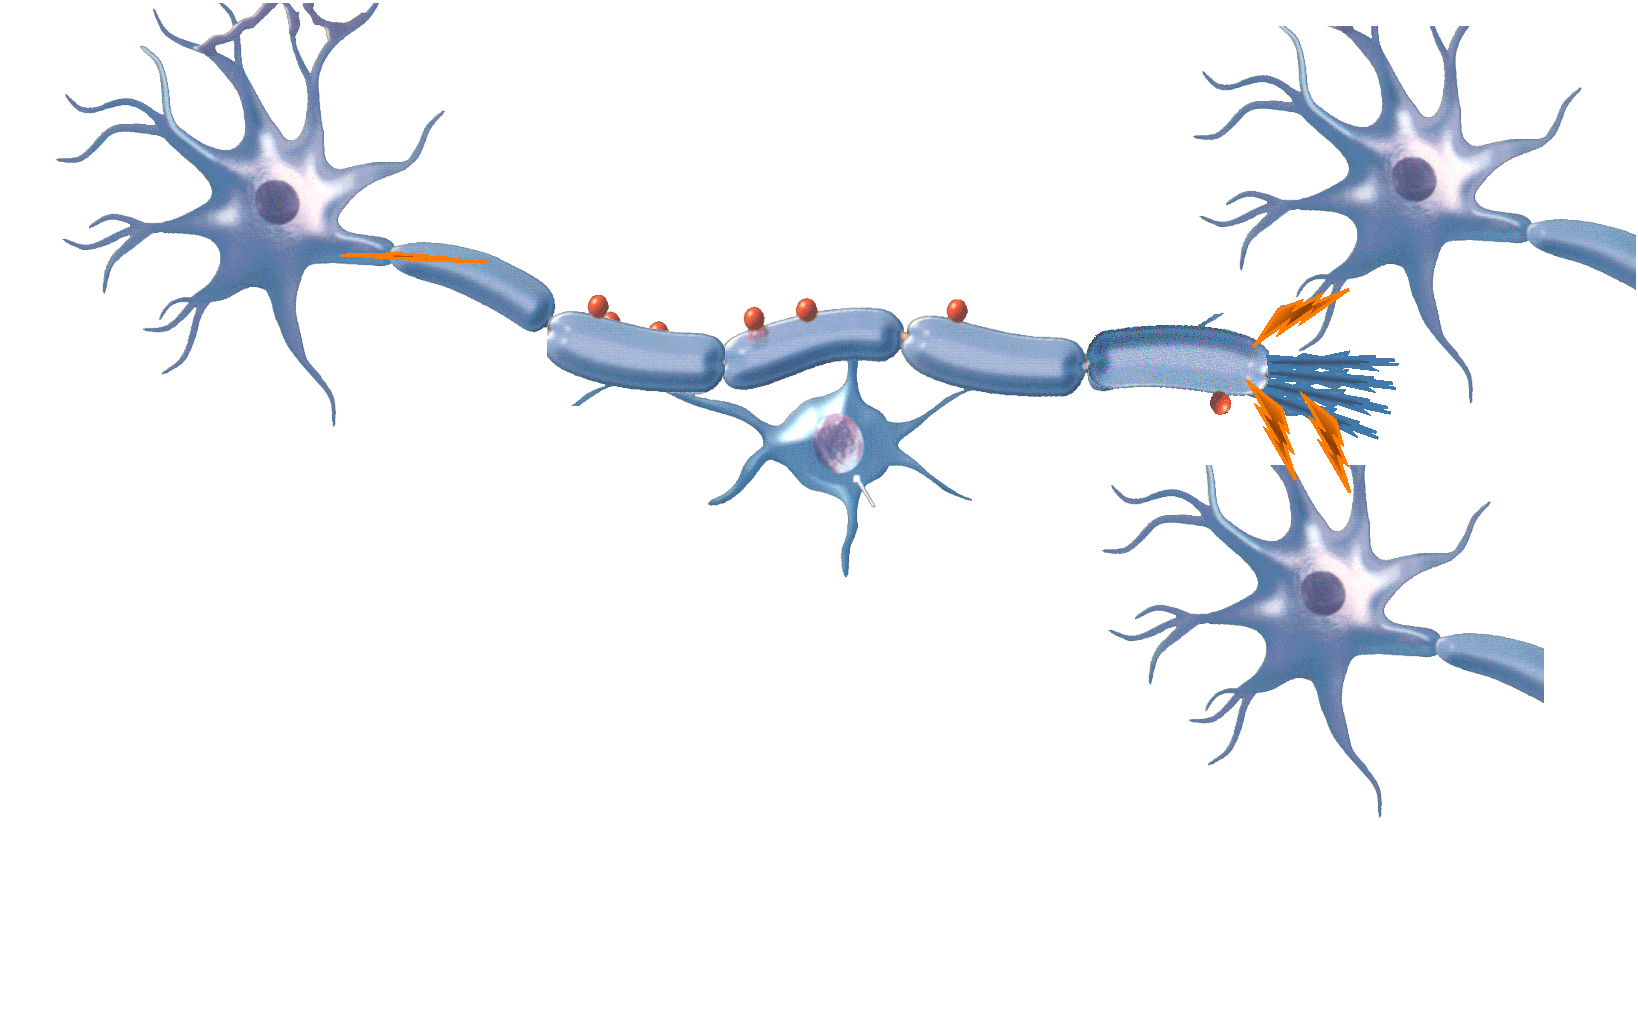
\includegraphics[width=0.5\textwidth]{figures/healthyneuron}};
\node[,below=-1.5cm of healthy] (damaged)
{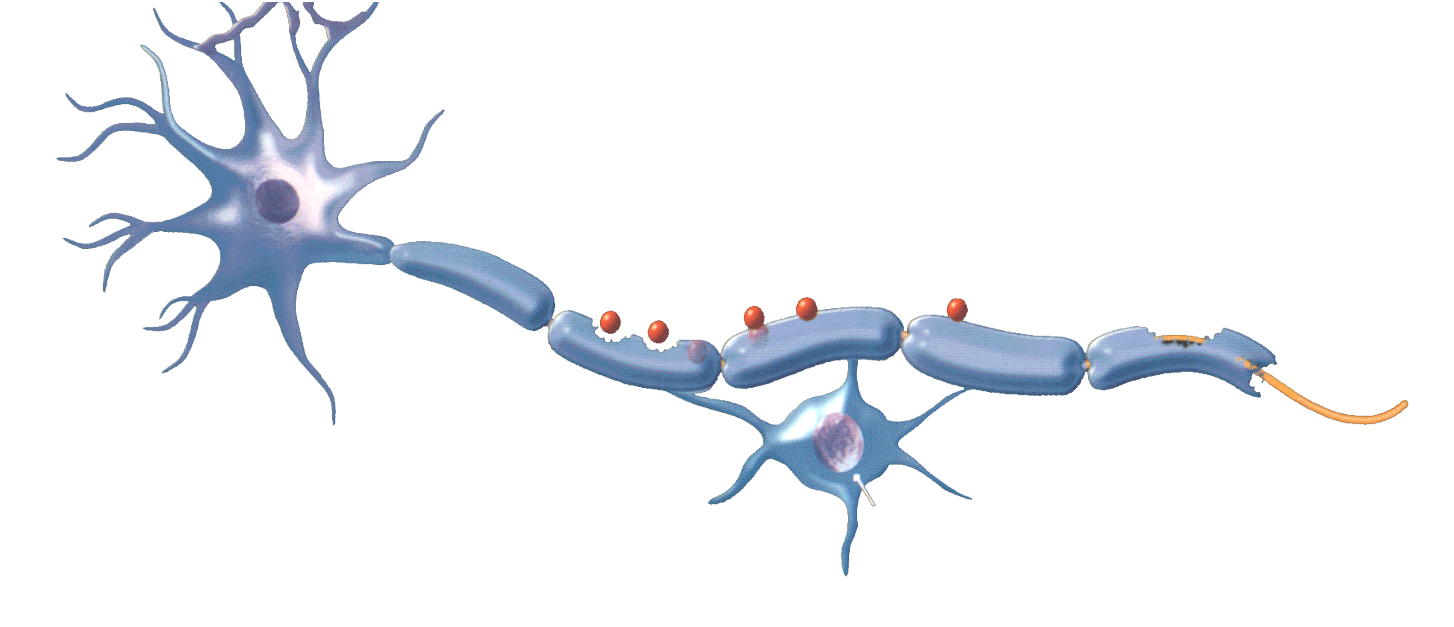
\includegraphics[width=0.5\textwidth]{figures/damagedneuron}};

\node[fit=(healthy)(damaged), inner sep=0] (neurons) {};

\node[right=1cm of neurons] (brain)
{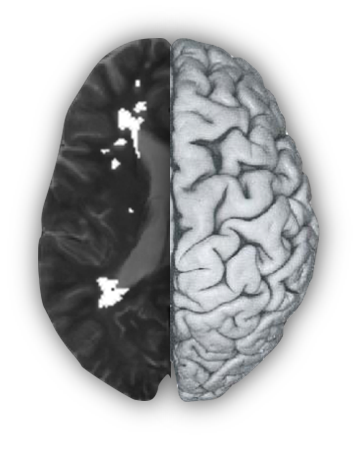
\includegraphics[width=0.4\textwidth]{figures/brain}};

\coordinate (m1) at (-0.75,0.9);
\coordinate (m2) at (0.95,0.9);
\coordinate (m3) at (2.4,-3);

\node[fit=(m1)(m2)] (myelin) {};

\node[above=0.65cm of myelin] (sheaths) {Myelin sheaths};

\draw (m1)--(sheaths);
\draw (m2)--(sheaths);

\node[ellipse,draw=red,thick,minimum width=1.5cm, minimum height=0.9cm,
label=90:Damaged myelin] at (m3) {};

\coordinate (wm) at (7.2,-0.5);
\coordinate (wml) at (6.9,-2.2);

%\draw[red] (wm) circle (3pt);
%\draw[red] (wml) circle (3pt);

\draw[gray,thick] (wm)--(healthy);
\draw[gray,thick] (wml)--(damaged);

%\draw[step=1cm,gray,very thin] (-5,2) grid (10,-6);

\end{tikzpicture}

\caption[Demyelination in MS]{Due to the break down of the blood brain barrier,
the body's own immune system attacks the myelin sheaths of the axons, which
causes the formation of demyelinating lesions, visible primarily in the white
matter on conventional \gls{mri} scans. Lesions are highlighted in white.}
\label{fig:ms}
\end{figure}
 
The clinical presentation of MS is very heterogeneous due to the wide range of
areas of the brain and spinal cord that can be affected. Characteristic but not
specific physical signs and symptoms include the loss of sensitivity or changes
in sensation such as tingling or numbness, which typically starts in the fingers
and toes, as well as muscle weakness, difficulty in moving, difficulties with
coordination and balance, problems with speech or swallowing, visual problems,
feeling tired, acute or chronic pain, and bladder and bowel difficulties. In
addition, MS often leads to cognitive problems such as having difficulties
learning and remembering information, or psychiatric and emotional problems such
as depression or frequent mood swings.

The course of the disease is unpredictable. Most patients (around
\SI{80}{\percent}) are initially diagnosed as having \gls{rrms}, which is
characterized by alternating periods of worsening due to inflammatory attacks
and the formation of new lesions, and periods of remission and recovery. The
majority (around \SI{65}{\percent}) of RRMS patients transition to \gls{spms}.
In this stage, the body is no longer able to compensate for the tissue damage,
which leads to the unremitting and progressive accumulation of disability. Other
types of MS include \glslink{ppms}{the primary progressive form (PPMS)},
characterized by the progression of disability from onset with no remissions
after the initial symptoms, and \gls{prms}, which shows progressive accumulation
of disability in addition to clear superimposed relapses.

\subsection[Measuring disease state and progression]{Measuring Disease State and
Progression}

There is currently no cure for MS. Existing therapies that focus on symptomatic
management and prevention of further damage have variable degrees of
effectiveness, although several recent breakthroughs are promising. To monitor
and further our understanding of the disease, many biomarkers have been
developed that allow for the objective measurement of normal and pathogenic
processes, as well as the monitoring of treatment effect. Current MS biomarkers
can be roughly classified into generic-immunogenetic, laboratorial, and imaging
biomarkers \citep{katsavos2013}. For this thesis, we focus on the accurate
measurement of existing lesion-based imaging biomarkers such as lesion volume
and lesion count, and the development of new biomarkers that capture changes in
brain morphology and white matter lesions---two hallmarks of MS pathology.

Accurate segmentation of MS lesions has shown to be a very challenging due to
the large variability in lesion size, shape, intensity, and locations, as well
as the large variability in imaging contrasts produced by scanners used at
different clinical sites. Despite a growing interest in developing fully
automatic lesion segmentation methods, semi-automatic methods are still the
standard in clinical research, although their use is time-consuming,
laborious, and potentially biasing. It is therefore highly desirable to develop
a fully-automatic lesion segmentation method that is robust to large
variability, while still being able to segment lesions with high accuracy and
sensitivity.

%
% - biomarkers based on the accurate delineation of lesions such as lesion count
%   and lesion volume
% - To measure those changes accurately, accurate segmentations of different
%   tissue types and lesions are required.
% - A lot of progress has been made to accurately separate the brain from
%   non-brain tissues (brain extraction) and segmenting the brain into its three
%   main tissue types, CSF, WM, GM.
% - Segmenting lesions very challenging due to the large variability in lesion
%   size, shape, contrast, and location as well the the large variability in
%   normal tissue contrasts produced by different scanners at different clinical
%   cites.
% - There is still no fully automatic and robust method for the segmentation of
%   lesions that is robust and accurate enough to be used in routine clinical
%   practice.

Imaging biomarkers used in clinical trials mostly focus on volumetric measures
of global and local changes, which are important and relatively easy to compute,
but only correlate modestly with clinical scores. One reason for the modest
correlation is that they do not reflect potentially important structural
variations, such as shape changes in the brain and the spatial dispersion of
lesions. Therefore, it would be highly desirable to develop biomarkers that
capture potentially important patterns of the variability in brain morphology
and lesion distribution, which would advance our understanding of the complex
pathology of MS.

% they only correlate modestly with clinical
% disability scores, which limits their utility for the purpose of personalized
% medicine. There are a number of key reasons why the current imaging biomarkers
% do not have stronger quantitative relationships with clinical scores:
% \begin{itemize}
% 
% \item Due to the wide range of symptoms, MS disability is difficult to score
% comprehensively in routine clinical practice. For example, the Kurtzke expanded
% disability status scale (EDSS)~\citep{Kurtzke:1983} is the most commonly used
% clinical score, but does not account for cognitive impairment, which is a
% significant contributor to disability in the majority of MS
% patients~\citep{Chiaravalloti:2008}.
% 
% \item Through neuroplasticity, the brain and spinal cord can adapt to damage in
% order to maintain functionality~\citep{Tomassini:2012}. As a result, clinically
% silent or subtle pathology is often present.
% 
% \item Conventional MRI does not capture all aspects of MS pathology. For
% example, white matter that appears normal on conventional MRI may actually have
% reduced myelin~\citep{Laule:2004}, a nerve insulator that is critical for proper
% signal conduction. Demyelination is a key pathological feature of MS.
% 
% \item The current established imaging biomarkers largely capture volumetric
% changes, which are important and relatively easy to compute, but do not reflect
% potentially important structural variations, such as shape changes in the brain
% and spatial dispersion of the lesions.
% 
% \end{itemize}
% It would be highly desirable to develop biomarkers that capture potentially
% important patterns of variability in brain morphology and lesion distribution,
% which would advance our understanding of the complex pathology of MS.

% An alternative to using biomarkers for monitoring MS is the use of clinical
% scores. In contrast to biomarkers, clinical scores measure the impact of the
% disease on the patient's life directly through clinical tests. The two most
% widely used scores of measuring disability in MS are the expanded disability
% status scale (EDSS) and the multiple sclerosis function composite. The EDSS
% provides a discrete scale of impairment to ambulation and ranges from 0 (normal
% neurological exam) to 10 (death due to MS). Despite its wide use in clinical
% trials, EDSS have been criticized for putting too much emphasise on the motor
% function of the patient, while ignoring other areas of the patient's life such
% as cognitive functions and upper body movement. The MSFC is a composite score
% composed of the following three subscores: 1) The timed 25 feet walk (T25W)
% measures impairment of the lower limbs, 2) the 9-hole peg test (9-HPT) measures
% impairment of the upper limbs, and 3) the paced auditory serial addition test
% (PASAT) measures impairment of the cognitive function of a patient.
% 
% - Scores don't correlate well with biomarkers
% - Why is this so?
% - Need better biomarkers
% - Maybe introduce clinical scores first then say biomarkers can be used as well
% - Difficulties measuring them
% - Difficulties with correlation to clinical scores

\section[Proposed method]{Proposed Method}

\subsection{Objectives}

% More general and taylored to the challenges. Robust method is the objective.
% Contribution is the development of a method based on neural networks and the
% contributions in there.

The clinical motivation of the thesis is to develop methods that facilitate the
automatic measurement of MS disease state and progression that are visible on
conventional structural MRIs. To that end, we have identified two key
applications. One is the development of a fully automatic lesion segmentation
method that is able to segment lesions over a large range of sizes and in the
presence of varying imaging contrasts and imaging artifacts produced by
different scanners, which would allow for the accurate measurement of
lesion-based imaging biomarkers such as lesion load and lesion count. The other
key application is the development of a method that automatically discovers
potentially important patterns of variability in brain morphology and lesion
distribution, with the goal to derive new imaging biomarkers that correlate
stronger with the clinical measures of MS disability than traditionally used
volumetric measures. The global objective of the thesis is to determine the
capabilities of deep learning \citep{lecun2015} for these two clinical
applications.

\subsection{Overview}

The two methods developed for segmenting MS lesions and modelling patterns of
variability are both based on deep learning, a field within machine learning
that is inspired by the learning capabilities of the brain. The human brain has
often served as a model for computer vision algorithms. For example, SIFT
features \citep{lowe1999}, inspired by neurons of the inferior temporal cortex,
have proved to be very robust for object recognition. Resembling the receptive
field of simple cells of the primary visual cortex, 2D Gabor filters have been
used to describe textures for segmentation \citep{grigorescu2002}. In contrast,
deep learning algorithms try to mimic how the visual system learns instead of
copying what it has learned. First evidence for the learning capabilities of the
visual system were found by \citep{wiesel1963}, who investigated the visual
cortex of cats. They showed that the receptive fields of neurons are learned
from a continuous stream of images early in the development of the visual system
\citep{wiesel1963}, but they are also fine-tuned later \citep{karni1991}.
This allows the neurons of the visual cortex to adapt to the type of images to
which it is exposed. While it is difficult, for example, for an average person
to recognize the differences between cows of the same breed, the feature
detecting neurons of the visual system of cattle farmers are highly tuned to
their appearance, allowing them to recognize individual cows easily. This
suggests that a learning-based model for classification should not only learn to
perform the requested task based on a set of pre-defined features, but also
learn the features that are most suitable to perform the task. The joint
learning of feature extraction and prediction, also known as end-to-end
learning, is possible through the use of deep learning methods, which use
multiple layers of nonlinear processing units to learn a feature hierarchy
directly from the input data without a dedicated feature extraction step.

Deep learning has successfully been used in many research areas such as object
recognition \citep{krizhevsky2012}, speech recognition \citep{hinton2012deep},
natural language understanding \citep{collobert2011natural}, and language
translation \citep{sutskever2014sequence}. Deep learning methods are
particularly successful due to their ability to recognize complex and highly
nonlinear patterns in large amounts of training data, which facilitates the
learning of models that are robust to large variability. This motivates the use
of deep learning methods for segmenting MS lesions, because the large
variability in lesion shape, size, contrast, and location as well as changes in
imaging contrasts produced by different \gls{mri} scanners make lesion
segmentation challenging. Beyond voxel classification, deep learning methods can
also be used to model highly nonlinear patterns of variability in groups of
images. This allows deep learning models such as deep belief networks to be used
for manifold learning, e.g., of hand written digits \citep{hinton2006b} or, as
we will show in \ref{sec:manifold}, brain MRIs \citep{brosch2013}. However,
deep learning algorithms as implemented by widely used deep learning frameworks
were originally developed for application to small 2D images and do not scale
well to large 3D volumes in terms of training time and memory requirements,
which prevents the use of out-of-the-box implementations for 3D medical image
analysis.

\subsection{Contributions}

In the course of developing deep learning-based methods for MS lesion
segmentation and pattern discovery, we have made the following main
contributions:
\begin{enumerate}
\item We have developed a novel training algorithm for convolutional deep belief
networks and convolutional neural networks that performs training in the
frequency domain. The speed-ups gained by our method compared to state-of-the
art spatial domain implementations and the reduced memory requirements compared
to other frequency domain methods enable the application of deep learning to
high-resolution 3D medical images.
  
\item We have developed a neural network architecture that jointly learns
features at different scales that are tuned to segmenting MS lesions and
performs the segmentation based on the automatically learned features. The joint
learning of feature extractor and classifier facilitates the learning of
features that are robust to the large variability of MS lesions and varying
contrasts produced by different scanners.

% \item In contrast to previous patch-based deep learning segmentation approaches,
% our network feeds through entire volumes, which removes the need to select
% representative patches, eliminates redundant calculations where patches overlap,
% and therefore scales up more efficiently with image resolution.

% There are many more contributions for segmentation than manifold
% learning; this should be more balanced. I suggest removing some the
% segmentation contributions so that you will have about 5 total contributions.
% As discussed, a main contribution in manifold learning is that you showed that
% deep learning can be applied to manifold learning of brain MRIs. Another is
% that joint learning can be performed to model key pathology features together,
% such as lesions and morphology.

% \item In contrast to previous fully convolutional deep learning segmentation
% approaches, our method produces segmentations of the same resolution and scale
% as the input images, independent of the parameters of the network architecture,
% which enables the use of deeper networks without requiring special handling
% of the border regions.

\item We have developed a novel objective function for training neural networks
that is suitable for the classification of vastly unbalanced classes, such as
the segmentation of MS lesions, which typically comprise less than one percent
of the image.

% \item Our proposed network architecture contains shortcut connections between
% the feature extraction and segmentation pathways, which allows for the learning
% of features at different scales and thereby facilitates the accurate
% segmentation of MS lesions across a wide range of sizes.

\item This is the first work to demonstrate that deep learning can be applied to
manifold learning of brain MRIs.

\item We have developed a framework for modelling changes in brain morphology
and lesion distribution with only a few parameters, which also show improved
correlation with clinical scores compared to established volumetric imaging
biomarkers.

% \item In contrast to previous manifold learning approaches, our method does not
% assume the ambient space to be locally linear and also does not require the
% definition of a suitable similarity measure, or building a proximity graph,
% which is particularly advantageous for modelling lesions, because their sparse
% and random nature makes defining a suitable distance measure between lesion
% images challenging.
\end{enumerate}

\section[Thesis outline]{Thesis Outline}

The rest of this thesis is organized into five chapters as outlined below:

\subsection*{\ref{sec:background}---\nameref{sec:background}}

In this chapter, we will briefly introduce the supervised and unsupervised deep
learning models that form the basis for the lesion segmentation and manifold
learning methods, which are discussed further in \ref{sec:segmentation}
and \ref{sec:manifold}. We will start with a description of dense neural
networks \citep{farley1954,werbos1974,rumelhart1986} and convolutional
neural networks \citep{fukushima1980,lecun1989,lecun1998}. In the second
part, we will give a brief overview of restricted Boltzmann Machines
\citep{freund1992,hinton2010a}, which are the building blocks of deep belief
networks \citep{hinton2006b}.

\subsection*{\ref{sec:training}---\nameref{sec:training}}

Deep learning has traditionally been computationally expensive and advances in
training methods have been the prerequisite for improving its efficiency in
order to expand its application to a variety of image classification problems.
In this chapter, we address the problem of efficient training of convolutional
deep belief networks by learning the weights in the frequency domain, which
eliminates the time-consuming calculation of convolutions. An essential
consideration in the design of the algorithm is to minimize the number of
transformations to and from frequency space. We have evaluated the running time
improvements using two standard benchmark data sets, showing a speed-up of up to
8 times on 2D images and up to 200 times on 3D volumes. In addition, we have
directly compared the time required to calculate convolutions using our method
with the \gls{cudnn}, the current state-of-the-art library for calculating 2D
and 3D convolutions, with the results showing that our method can calculate
convolutions up to 20 times faster than cuDNN. Our training algorithm makes
training of convolutional deep belief networks and convolutional neural networks
on 3D volumes with a resolution of up to \num{128x128x128} voxels
practical, which opens new directions for using deep learning for medical image
analysis.

\subsection*{\ref{sec:segmentation}---\nameref{sec:segmentation}}

In this chapter, we present a novel segmentation approach based on deep 3D
convolutional encoder networks with shortcut connections and apply it to the
segmentation of MS lesions in magnetic resonance images. Our model is a neural
network that consists of two interconnected pathways, a convolutional pathway,
which learns increasingly more abstract and higher-level image features, and a
deconvolutional pathway, which predicts the final segmentation at the voxel
level. The joint training of the feature extraction and prediction pathways
allows for the automatic learning of features at different scales that are
optimized for accuracy for any given combination of image types and segmentation
task. In addition, shortcut connections between the two pathways allow high- and
low-level features to be integrated, which enables the segmentation of lesions
across a wide range of sizes. We have evaluated our method on two publicly
available data sets (MICCAI 2008 and ISBI 2015 challenges) with the results
showing that our method performs comparably to the top-ranked state-of-the-art
methods, even when only relatively small data sets are available for training.
In addition, we have compared our method with five freely available and widely
used MS lesion segmentation methods (EMS, LST-LPA, LST-LGA, Lesion-TOADS, and
SLS) on a large data set from an MS clinical trial.
The results show that our method consistently outperforms these other methods
across a wide range of lesion sizes.

\subsection*{\ref{sec:manifold}---\nameref{sec:manifold}}

Manifold learning of medical images plays a potentially important role for
modelling anatomical variability within a population with applications that
include segmentation, registration, and prediction of clinical parameters.
In this chapter, we describe a novel method for learning the manifold of 3D
brain images and for building a statistical model of brain images that can
automatically discover spatial patterns of variability in brain morphology and
lesion distribution. We propose building such a model using a deep belief
network, a layered network whose parameters can be learned from training
images. In contrast to other manifold learning algorithms, this approach does
not require a prebuilt proximity graph, which is particularly advantageous for
modelling lesions, because their sparse and random nature makes defining a
suitable distance measure between lesion images challenging. Our results show
that this model can automatically learn a low-dimensional manifold of brain
volumes that detects modes of variations that correlate to demographic and
disease parameters. Furthermore, our model can automatically discover the
classic patterns of MS pathology, as well as more subtle ones, and the
computed parameters have strong relationships to MS clinical scores.

\subsection*{\ref{sec:conclusions}---\nameref{sec:conclusions}}

This chapter concludes the thesis with a brief summary of the problems addressed
and key results. In addition, some directions for future work are given in the
broader context of deep learning for medical imaging. In particular, we will
give suggestions for new medical image analysis applications of deep learning
and how to deal with relatively small data sets using data augmentation. In
addition, we will discuss two potential advancements of neural networks that we
believe will be particularly important for medical applications.

%   - Use more data, handle variability better, age of large data is perfect for deep learning
%   - No assumptions other than test data should be similarly distributed than training data -> robust and fast
%   - What can we learn from it? Need visualization of what the network is thinking. Probably relearn what the NN is doing similar to how 
%     brain research works: learn from good and bad cases or from deactivating certain parts of the network to infer what it does.
%   - Theory of learning combining neuroscience and computer science

\begin{comment}

Multiple sclerosis (MS) is a chronic, degenerative disease of the brain and
spinal cord. The clinical presentation of MS is very heterogeneous, and the
range and severity of symptoms can vary greatly between patients. The clinical
course of MS is highly unpredictable, but most patients are initially diagnosed
as having relapsing remitting MS (RRMS), which is characterized by inflammatory
attacks separated by variable periods of remission and recovery. The majority of
RRMS patients will eventually transition into the secondary progressive MS
(SPMS) phase, in which there is an unremitting and progressive accumulation of
disability. There is currently no cure for MS. Existing therapies that focus on
symptomatic management and prevention of further damage have variable degrees of
effectiveness, although several recent breakthroughs are promising. MS pathology
originates at the cellular level and many aspects are not well understood, but
there are characteristic (but not specific) signs of tissue damage, the most
recognizable of which are white matter lesions (WMLs) and brain atrophy, or
shrinkage due to degeneration. These signs can be observed on MRI, which has
become a vital tool for non-invasively monitoring MS patients in the clinic and
for advancing the understanding of MS pathology. WML counts and volume and brain
volume have become established imaging biomarkers for MS clinical trials, and
there is promise for their use in routine clinical practice, but they generally
only correlate modestly with clinical disability scores. The weak link between
the image-based measures of MS pathology and disability scores is known as the
``clinico-radiological paradox'' of MS, and results in the low utility of
current imaging biomarkers for the purposes of personalized medicine. There are
a number of key reasons why the current imaging biomarkers do not have stronger
quantitative relationships with clinical scores:

\begin{itemize}

\item Due to the wide range of symptoms, MS disability is difficult to score
comprehensively in routine clinical practice. For example, the Kurtzke expanded
disability status scale (EDSS)~\citep{Kurtzke:1983} is the most commonly used
clinical score, but does not account for cognitive impairment, which is a
significant contributor to disability in the majority of MS
patients~\citep{Chiaravalloti:2008}.

\item Through neuroplasticity, the brain and spinal cord can adapt to damage in
order to maintain functionality~\citep{Tomassini:2012}. As a result, clinically
silent or subtle pathology is often present.

\item Conventional MRI does not capture all aspects of MS pathology. For
example, white matter that appears normal on conventional MRI may actually have
reduced myelin~\citep{Laule:2004}, a nerve insulator that is critical for proper
signal conduction. Demyelination is a key pathological feature of MS.

\item The current established imaging biomarkers largely capture volumetric
changes, which are important and relatively easy to compute, but do not reflect
potentially important structural variations, such as shape changes in the brain
and spatial dispersion of the lesions.

\item Traditional statistical approaches place a strong emphasis on
interpretability, often at the sacrifice of accuracy, and simple prediction
models such as logistic regression are common. The general assumption is that
the data is generated by a known stochastic data model, with the goodness-of-fit
evaluated by residual analysis, but this works well only with a very low number
of variables~\citep{Breiman2001}.

\end{itemize}

% Add to manifold introduction
Changes in brain morphology and white matter lesions are two hallmarks of MS
pathology, but their variability beyond volumetrics is poorly characterized. To
further the understanding of complex MS pathology,

% Add to segmentation introduction
Focal lesions in the brain and spinal cord are one of the hallmarks of MS
pathology, and are primarily visible in the white matter on structural MRIs.
These lesions are observable as hyperintensities on T2w, proton density-weighted
(PDw), or fluid-attenuated inversion recovery (FLAIR) scans, and as
hypointensities, or ``black holes'' on T1w scans. Imaging biomarkers based on
the identification of lesions, such as lesion count and lesion volume, have
established their importance for assessing disease progression and treatment
effect. However, lesions vary greatly in size, shape, intensity and location,
which makes their automatic and accurate segmentation challenging.

% See literature review as a tool, not as a goal. Try to structure the thesis
% without it and put it where it belongs. Maybe restructure later. I needed a part
% of it already for the motivation. I will put a lot in it when I describe the
% methods. An I will put something in there, when I describe the applications.

\end{comment}
\chapter{Background: Deep Learning}
\label{sec:background}

Deep learning is a field within machine learning that has been studied since the
early 1980s \citep{fukushima1980}. However, deep learning methods did not gain
in popularity until the late 2000s with the advent of fast general purpose
graphics processors \citep{raina2009}, layerwise pre-training methods
\citep{hinton2006b,hinton2006c}, and large data sets
\citep{deng2009,krizhevsky2012}. Since then, deep learning methods have become
the state-of-the-art in many non-medical \citep{krizhevsky2012,sainath2013} and
medical \citep{ciresan2012,kamnitsas2015} applications. There are many different
algorithms and models that are commonly referred to as deep learning methods,
all of which have two properties in common: 1) the use of multiple layers of
nonlinear processing units for extracting features, and 2) the layers are
organized to form a hierarchy of low-level to high-level features. Representing
data in a feature hierarchy has many advantages for classification and other
applications. To give an example of a feature hierarchy, let us consider the
domain of face images. The lowest layer of the feature hierarchy is composed of
the raw pixel intensities, which are the most basic features of an image.
Multiple pixels can be grouped to form general image features like edges and
corners, which can be further combined to form face parts such as different
variations of noses, eyes, mouths, and ears.
Finally, multiple face parts can be combined to form a variety of face images.
Learning a feature hierarchy facilitates the parameterization of a large feature
space with a small number of values by capturing complex relationships between
feature layers. For example, a feature hierarchy consisting of three
prototypical shapes for mouths, eyes, ears, and noses is able to represent
$\num{3x3x3x3} = 81$ different prototypical faces with only $3+3+3+3=12$
features. Without a hierarchical representation of the data, a model would
require $81$ prototypical face features to span the same face manifold.

In this chapter, we will briefly introduce the supervised and unsupervised deep
learning models that form the basis for the lesion segmentation and manifold
learning methods, which are discussed further in \ref{sec:segmentation} and
\ref{sec:manifold}. We will start with a description of \glspl{dnn}
\citep{farley1954,werbos1974,rumelhart1986} and \glspl{cnn}
\citep{fukushima1980,lecun1989,lecun1998}. In the second part, we will give a
brief overview of \glspl{rbm} \citep{freund1992,hinton2010a}, which are the
building blocks of \glspl{dbn} \citep{hinton2006b}.

% Reduce overlap with introduction)

% RBMs, DBNs, convRBMs, convDBNs for manifold learning and NN and CNN for lesion
% segmentation.

\section[Supervised learning]{Supervised Learning}

% If I put this first, I can argue with inspiration from biological models
% first.

A typical pipeline for classifying images consists of two main steps. In the
first step, predefined or learned features are extracted from the input images,
which are then used to train a separate supervised learning model, such as a
\gls{rf} \citep{breiman2001} or a \gls{svm} \citep{cortes1995},
to perform classification or prediction. Alternatively, classification and
prediction can be performed with a single model that takes the raw input data
and produces the desired output, such as class probabilities. This type of
learning is called end-to-end learning and has shown great potential for medical
image analysis \citep{ciresan2012}. The most popular models for end-to-end
learning are neural networks due to their ability to learn a hierarchical set of
features from raw input data. This allows the learning of features that are
tuned for a given combination of input modalities and classification task, but
is more prone to overfitting than unsupervised feature learning methods,
especially when the amount of labeled data is limited. In this section, we will
start with an introduction to dense neural networks, followed by a concise
overview of convolutional neural networks.

% \begin{itemize}
%   \item Extracted features often fed into a supervised model to perform
%   classification or prediction
%   \item Directly learn the mapping from raw input to final output, without a
%   separated feature extraction step
%   \item Called end-to-end learning
%   \item Multi-layer neural network
%   \item First layers learn to extract features from the input data
%   \item Last layers learn to classify the input
%   \item Minimize the error through backpropagation through all layers yields
%   feature extractor that is tuned to the classification task
%   \item Two types of neural networks are most common: dense neural networks
%   (DNN) and convolutional neural networks (CNN)
% \end{itemize}

\subsection[Dense neural networks]{Dense Neural Networks}
\label{sec:DNN}

A dense neural network (see \ref{fig:dnn}) is a deterministic function that maps
input data to the desired outputs through the successive application of multiple
nonlinear mappings of the following form
\begin{align}
\vect{z}_l &= \vect{W}_l\vect{x}_{l-1} + \vect{b}_l, \\
\vect{x}_l &= f_l(\vect{z}_l),
\end{align}
where $\vect{x}_l$ denotes a vector containing the units of layer $l$,
$\vect{x}_0$ denotes a vector containing the input of the neural network,
$\vect{x}_L$ denotes a vector containing the output, $L$ is the number of
computational layers, $f_l$ are transfer functions, $\vect{W}_l$ are weight
matrices, and $\vect{b}_l$ are bias terms. Popular choices for the transfer
function are the sigmoid function $f(x) = \sigm(x)$ and the rectified linear
function $f(x) = \max(0, x)$. The same transfer function is typically used for
all layers except for the output layer. The choice of the output transfer
function depends on the learning task. For classification, a $1$-of-$n$ encoding
of the output class is usually used in combination with the softmax transfer
function defined as
\begin{equation}
\text{softmax}(\vect{a})_i = \frac{\exp(a_i)}{\sum_{j=1}^n \exp(a_j)},
\end{equation}
where $\vect{a}$ denotes an $n$-dimensional output vector.

\begin{figure}
\centering
\begin{tikzpicture}
\tikzstyle{aenode}=[circle,draw,minimum width=0.5cm]
\tikzstyle{gnode}=[circle,draw,minimum width=0.5cm,dotted]

\foreach \y in {1,...,4} {
  \node[aenode] (inode\y) at (0, \y) {};
}

\begin{scope}[yshift=0.5cm]
\foreach \y in {1,...,3} {
  \node[aenode] (h1node\y) at (1.25, \y) {};
}
\end{scope}

\foreach \y in {1,...,4} {
  \node[gnode] (h2node\y) at (2.5, \y) {};
}

\begin{scope}[yshift=0.5cm]
\foreach \y in {1,...,3} {
  \node[aenode] (h3node\y) at (3.75, \y) {};
}
\end{scope}

\foreach \y in {1,...,4} {
  \node[aenode] (onode\y) at (5, \y) {};
}

\foreach \x in {1,...,4} {
  \foreach \y in {1,...,3} {
    \draw[-latex] (inode\x)--(h1node\y);
    \draw[-latex,dotted] (h1node\y)--(h2node\x);
    \draw[-latex,dotted] (h2node\x)--(h3node\y);
    \draw[-latex] (h3node\y)--(onode\x);
  }
}

\node[above=3pt of inode4] {$\vect{x}_0$};
\node[above=3pt of h1node3] {$\vect{x}_1$};
\node[above=3pt of h2node4] (xl) {$\vect{x}_l$};
\node[above=3pt of h3node3] {$\vect{x}_{L-1}$};
\node[above=3pt of onode4] {$\vect{x}_L$};

% \node at (xl-|inode1) {$\vect{x}_0$};
% \node at (xl-|h1node1) {$\vect{x}_1$};
% \node at (xl-|h3node1) {$\vect{x}_{L-1}$};
% \node at (xl-|onode1) {$\vect{x}_L$};

\path (h1node3)--node[above=2pt] {$\vect{W}_l$} (h2node4);

\node[below=5pt of h2node1] (hiddens) {Hidden units};
\node at (hiddens-|inode1) {Input units};
\node at (hiddens-|onode1) {Output units};

% \begin{scope}[decoration={brace,pre=moveto,pre length=1pt,post=moveto,post
% length=1pt}]
% 
% % Units
% \draw[decorate] ([xshift=0.5cm]inode4.east|-inode4.north)--
% node[right=4pt]{Input units $\vect{x}_0$}
% ([xshift=0.5cm]inode4.east|-inode4.south);
% 
% \draw[decorate] ([xshift=0.5cm]inode4.east|-hnode3.north)--
% node[right=4pt]{Hidden units $\vect{x}_1$}
% ([xshift=0.5cm]inode4.east|-hnode3.south);
% 
% \draw[decorate] ([xshift=0.5cm]onode4.east|-onode4.north)--
% node[right=4pt]{Reconstructions $\vect{x}_2$}
% ([xshift=0.5cm]onode4.east|-onode4.south);
% 
% \draw[decorate] ([xshift=0.5cm]onode4.east|-hnode3.south)--
% node[right=4pt]{Encoding weights $\vect{W}_1$}
% ([xshift=0.5cm]onode4.east|-inode4.north);
% 
% \draw[decorate] ([xshift=0.5cm]onode4.east|-onode4.south)--
% node[right=4pt]{Decoding weights $\vect{W}_2$}
% ([xshift=0.5cm]onode4.east|-hnode3.north);
% 
% \end{scope}
\end{tikzpicture}

\caption[Schematic depiction for the calculations in a dense neural
network]{Schematic depiction for the calculations in a dense neural network.
Each hidden and output unit calculates the weighted sum of its inputs followed
by the application of a transfer function.}
\label{fig:dnn}
\end{figure}

Given a training set $\data = \{(\vect{x}_0^{(i)}, \vect{y}^{(i)})\given i
\in [1, N] \}$, a neural network is trained by minimizing the error
between the predicted outputs $\vect{x}_L^{(i)}$ and the given labels
$\vect{y}^{(i)}$
\begin{equation}
\hat{\thetas} = \arg\min_{\thetas} \sum_{i = 1}^N E\Big(\vect{x}_L^{(i)},
\vect{y}^{(i)}\Big),
\end{equation}
where $\thetas$ denotes the trainable parameters of the neural network. Typical
choices for the error function are the \gls{ssd} and the cross-entropy.
The minimization problem can be solved using \gls{sgd}
\citep{rumelhart1986,polyak1992}, which requires the calculation of the gradient
of the error function with respect to the model parameters. The gradient can be
calculated by backpropagation \citep{werbos1974} as follows
\begin{align}
\deltas_L &= \nabla_{\vect{x}_L}E \cdot f_L'(\vect{z}_L), \\
\deltas_l &= (\vect{W}_{l+1}^\text{T}\deltas_{l+1}) \cdot
f_l'(\vect{z}_l) & \text{for $l < L$,}\\
\nabla_{\vect{W}_l}E &= \deltas_l\vect{x}_{l-1}^\text{T}, \\
\nabla_{\vect{b}_l}E &= \deltas_l,
\end{align}
where $\nabla_{\vect{x}_L}E$ denotes the gradient of the error function with
respect to the predicted output and $\cdot$ denotes element-wise multiplication.

\subsection[Convolutional neural networks]{Convolutional Neural Networks}

The structure of CNNs is inspired by the complex arrangement of simple and
complex cells found in the visual cortex \citep{hubel1962,hubel1968}. Simple
cells are only connected to a small sub-region of the previous layer and need to
be tiled to cover the entire visual field. In a CNN (see \ref{fig:cnn}),
simple cells are represented by convolutional layers, which exhibit a similar
mechanism of local connectivity and weight sharing. Complex cells combine the
activations of simple cells to add robustness to small translations. These cells
are represented in the form of pooling layers. After several alternating
convolutional and pooling layers, the activations of the last convolutional
layer are fed into one or more dense layers to carry out the final
classification.

\begin{figure}
\centering
\begin{tikzpicture}[%
scale=0.85,
x  = {(1cm,0cm)},
y  = {(0.33cm,0.23cm)},
z  = {(0cm,1cm)}
%z  = {(0.9cm,-0.1cm)},
%x  = {(0.33cm,0.23cm)},
%y  = {(0cm,1cm)}
]

\tikzstyle{every node}=[font=\small, inner sep=3pt, align=center]
\tikzstyle{every pin}=[align=center,fill=white]
\tikzstyle{dbnlabel}=[font=\sffamily\normalsize]

\tikzstyle{image}=[fill=white, fill opacity=0.75]
\tikzstyle{pinline}=[thin, black!35]
\tikzstyle{kernelline}=[very thin]


%%%%%%%%%%%%%%%%%         
% INPUT LAYER
%%%%%%%%%%%%%%%%%

\foreach \x in {1, ..., 3} {
\def\y{0.25*\x}
\draw[image] (\y, -2,-2) coordinate (A1\x) -- (\y, 2,-2)
coordinate (B1\x) -- (\y, 2,2) coordinate (C1\x) -- (\y, -2,2) -- cycle;

\draw[kernelline]
      (\y, -1.6, 1.6) \ifnum\x=3 \else -- +(0.25, 0, 0) +(0,0,0) \fi
   -- (\y, -0.8, 1.6) \ifnum\x=3 \else -- +(0.25, 0, 0) +(0,0,0) \fi
   -- (\y, -0.8, 0.8) \ifnum\x=3 \else -- +(0.25, 0, 0) +(0,0,0) \fi
   -- (\y, -1.6, 0.8) \ifnum\x=3 \else -- +(0.25, 0, 0) +(0,0,0) \fi
   -- (\y, -1.6, 1.6);
   ;
\ifnum\x=3
\draw[kernelline] (\y, -1.6, 1.6) coordinate(a1) -- (1.65, -1.2, 1.2);
\draw[kernelline] (\y, -1.6, 0.8) coordinate(b1) -- (1.65, -1.2, 1.2);
\draw[kernelline] (\y, -0.8, 0.8) coordinate(c1) -- (1.65, -1.2, 1.2);
\draw[kernelline] (\y, -0.8, 1.6) coordinate(d1) -- (1.65, -1.2, 1.2);
\fi
}

%%%%%%%%%%%%%%%%%         
% HIDDEN LAYER
%%%%%%%%%%%%%%%%%

\foreach \x in {0, ..., 7} {
\def\y{0.125*\x+1.65}
\draw[image] (\y,-1.6,-1.6) coordinate(A2\x) -- (\y,1.6,-1.6)
-- (\y,1.6,1.6) coordinate (C2\x) -- (\y,-1.6,1.6) coordinate(D2\x) -- cycle;

\draw[kernelline]
      (\y, -0.8, 0.8) \ifnum\x=7 \else -- +(0.125, 0, 0) +(0,0) \fi
   -- (\y, -0.4, 0.8) \ifnum\x=7 \else -- +(0.125, 0, 0) +(0,0) \fi
   -- (\y, -0.4, 0.4) \ifnum\x=7 \else -- +(0.125, 0, 0) +(0,0) \fi
   -- (\y, -0.8, 0.4) \ifnum\x=7 \else -- +(0.125, 0, 0) +(0,0) \fi
   -- (\y, -0.8, 0.8);
\ifnum\x=7
\draw[kernelline] (\y, -0.8, 0.8) coordinate(a2) -- (3.425, -0.6, 0.6);
\draw[kernelline] (\y, -0.8, 0.4) coordinate(b2) -- (3.425, -0.6, 0.6);
\draw[kernelline] (\y, -0.4, 0.4) coordinate(c2) -- (3.425, -0.6, 0.6);
\draw[kernelline] (\y, -0.4, 0.8) coordinate(d2) -- (3.425, -0.6, 0.6);
\fi 
}

\draw[decorate,decoration={brace,raise=20pt}] (A11|-C11) --node[above=25pt]
{Convolutional layer} (C27|-C11);

\foreach \x in {0, ..., 7} {
\def\y{0.125*\x+3.425}
\draw[image] (\y,-0.8,-0.8) coordinate(A3\x) -- (\y,0.8,-0.8)
-- (\y,0.8,0.8) coordinate (C3\x) -- (\y,-0.8,0.8) -- cycle;

\draw[kernelline]
      (\y, -0.6, +0.6) \ifnum\x=7 \else -- +(0.125, 0, 0) +(0,0) \fi
   -- (\y, +0.2, +0.6) \ifnum\x=7 \else -- +(0.125, 0, 0) +(0,0) \fi
   -- (\y, +0.2, -0.2) \ifnum\x=7 \else -- +(0.125, 0, 0) +(0,0) \fi
   -- (\y, -0.6, -0.2) \ifnum\x=7 \else -- +(0.125, 0, 0) +(0,0) \fi
   -- (\y, -0.6, +0.6);
\ifnum\x=7
\draw[kernelline] (\y, -0.6, +0.6) -- (5.2, -0.2, 0.2);
\draw[kernelline] (\y, -0.6, -0.2) -- (5.2, -0.2, 0.2);
\draw[kernelline] (\y, +0.2, -0.2) coordinate (g7) -- (5.2, -0.2, 0.2);
\draw[kernelline] (\y, +0.2, +0.6) -- (5.2, -0.2, 0.2);
\fi 
}

\draw[decorate,decoration={brace,raise=10pt}] (C21|-C21) --node[above=15pt]
{Pooling layer} (C37|-C21);

\foreach \x in {0, ..., 15} {
\def\y{0.125*\x+5.2}
\draw[image] (\y,-0.4,-0.4) coordinate (A4\x) -- (\y,0.4,-0.4)
-- (\y,0.4,0.4) coordinate (C4\x) -- (\y,-0.4,0.4) -- cycle;
}

\begin{scope}[xshift=9cm]
\foreach \x in {1,...,7} {
  \node[circle, draw] (v\x) at (0,0, 0.5*\x - 0.5*4) {};
}
\end{scope}

\draw[shorten >=10pt,shorten <=7pt,dashed] (A415-|C415)--(v1.south west);
\draw[shorten >=10pt,shorten <=7pt,dashed] (C415)--
node[label=120:Vectorize\\ hidden units] {} (v7.north west);

\begin{scope}[xshift=10.5cm]
%\foreach \x/\y in {1/-1.5, 2/-1, 3/-0.5, 4/0, 5/0.5, 6/1, 7/1.5} {
\foreach \x in {1,...,5} {
  \node[circle, draw] (h\x) at (0,0, 0.5*\x - 0.5*3) {};
}
\end{scope}

\foreach \x in {1,...,7} {
	\foreach \y in {1,...,5} {
		\draw (v\x)--(h\y);
	}
}

\draw[decorate,decoration={brace,raise=10pt}] (v7.west|-C21)
 --node[above=15pt] {Dense layer} (h1.east|-C21);
 
\node[above=15pt, fill=white,xshift=-25pt,inner sep=3pt, fill opacity=1, text
opacity=1] 
(convl) at (d1) {convolution};
\draw[pinline, shorten >=4pt, shorten <=2pt] (convl) -- (d1);

\node[above=15pt,fill=white,xshift=35pt,inner sep=3pt]
(pooll) at (d2) {pooling};
\draw[pinline, shorten >=4pt, shorten <=2pt] (pooll) -- (d2);

% Label units

\node[below=10pt,align=center] (input) at (A12) {Multimodal\\ input images};

\draw[pinline, shorten >=4pt] (input) -- (A11);
\draw[pinline, shorten >=4pt] (input) -- (A12);
\draw[pinline, shorten >=4pt] (input) -- (A13);

\node[below=40pt,xshift=20pt,inner sep=5pt] (hiddens) at (A31) {Hidden units};
\draw[pinline, shorten >=4pt] (hiddens) -- (A27);
\draw[pinline, shorten >=4pt] (hiddens) -- (A34);
\draw[pinline, shorten >=4pt] (hiddens) -- (A47);
\draw[pinline, shorten >=4pt] (hiddens) -- (v1);

\node[below=25pt,align=center] (output) at (h1) {Output\\ units};
\draw[pinline, shorten >=4pt] (output) -- (h1);

\begin{comment}

%%%%%%%%%%%%%%%%%         
% OUTPUT LAYER
%%%%%%%%%%%%%%%%%

\begin{scope}[canvas is xy plane at z=3.425]
\draw[image] (-2,-2) coordinate (A) -- (2,-2)
-- (2,2) coordinate (C) -- (-2,2) -- cycle;
\end{scope}

\node[xshift=-0.7cm, left] (lesion) at (A) {$S$};
\draw[pinline, shorten >=4pt] (lesion) -- (A);

\node[xshift=0.7cm, right] (y2) at (C) {$y^{(2)}$};
\draw[pinline, shorten <=4pt] (C) -- (y2);

\draw[decorate,decoration={brace,raise=75pt,mirror}] (B1-|C) --
node[right=80pt] {Convolutional\\ network} (G7-|C1);

\draw[decorate,decoration={brace,raise=95pt,mirror}] (G0-|C1) --
node[right=100pt] {Deconvolutional\\ network} (C);

\end{comment}

\end{tikzpicture}
%\includegraphics{figures/Fig-3-3}
\caption[Convolutional neural network with two convolutional layers, one pooling
layer and one dense layer]{Convolutional neural network with two convolutional layers, one
pooling layer and one dense layer. The activations of the last layer are the
output of the network.}
\label{fig:cnn}
\end{figure}

For multimodal $3$D volumes, the neurons of convolutional and pooling layers are
arranged in a $4$D array, where the first three dimensions correspond to the
dimensions of the input volume, and the forth dimension indexes the input
modality or channel. The activations of the output of a convolutional layer are
calculated by
\begin{equation}
x^{(l)}_j = f\Bigg(\sum_{i=1}^C\tilde{w}^{(l)}_{ij}*x^{(l-1)}_i
+ b^{(l)}_j\Bigg),
\end{equation}
where $l$ is the index of a convolutional layer, $x^{(l)}_j$ denotes the $j$th
channel of the output volume, $w^{(l)}_{ij}$ is a $3$D filter kernel connecting
the $i$th channel of the input volume to the $j$th channel of the output volume,
$b_j^{(l)}$ denotes the bias term of the $j$th output channel, and $\tilde{w}$
denotes a flipped version of $w$, i.e. $\tilde{w}(a) = w(-a)$. CNNs can be
trained using stochastic gradient descent, where the gradient can be derived
analogously to dense neural networks and calculated using backpropagation
\citep{lecun1989,lecun1998}.

Different types of operations \citep{scherer2010} have been proposed for the
pooling layers, with the common goal of creating a more compact representation
of the input data. The most commonly used type of pooling is max-pooling.
Therefore, the input to the pooling layer is divided into small blocks and only
the maximum value of each block as passed on to the next layer, which makes the
representation of the input invariant to small translations in addition to
reducing its dimensionality.

A major challenge for gradient-based optimization methods is the choice of an
appropriate learning rate. Classic stochastic gradient descent \citep{lecun1998}
uses a fixed or decaying learning rate, which is the same for all parameters of
the model. However, the partial derivatives of parameters of different layers
can vary substantially in magnitude, which can require different learning rates.
In recent years, there has been an increasing interest in developing methods for
automatically choosing independent learning rates. Most methods (e.g., AdaGrad
by \citealp{duchi2011}; AdaDelta by \citealp{zeiler2012}; RMSprop
by \citealp{dauphin2015}; and Adam by \citealp{kingma2014}) collect different
statistics of the partial derivatives over multiple iterations and use this
information to set an adaptive learning rate for each parameter. This is
especially important for the training of deep networks, where the optimal
learning rates often differ greatly for each layer.

\section[Unsupervised learning]{Unsupervised Learning}

% More statistical learning and finding patterns of similarity.

One of the most important applications of deep learning is to learn patterns of
variability in the form of a feature hierarchy from unlabeled images. The key to
learning such a hierarchy is the ability of deep models to be trained layer by
layer, where each layer acts as a nonlinear feature extractor. Various methods
have been proposed for feature extraction from unlabeled images. In this
section, we will first introduce the restricted Boltzmann machines
\citep{freund1992,hinton2010a}, which are the building blocks of the later
described deep belief networks \citep{hinton2006b}.

\subsection[From restricted Boltzmann machines to deep belief networks]{From
Restricted Boltzmann Machines to Deep Belief Networks}

An RBM is a probabilistic graphical model defined by a bipartite graph as shown
in \ref{fig:rbm}. The units of the RBM are divided into two layers, one of
visible units $\vect{v}$ and the other of hidden units $\vect{h}$. There are no
direct connections between units within either layer. An RBM defines the joint
probability of visible and hidden units in terms of the energy $E$,
\begin{align}
p(\vect{v}, \vect{h} \given \thetas) &=
\frac{1}{Z(\thetas)}e^{-E(\vect{v}, \vect{h} \given \thetas)}. \\
\intertext{When the visible and hidden units are binary, the energy is defined
as} 
-E(\vect{v}, \vect{h}\given \thetas) &= \sum_{i, j}v_i w_{ij} h_j +
\sum_i b_i v_i + \sum_j c_j h_j, \\
&= \vect{v}^\textup{T}\vect{W}\vect{h} + \vect{b}^\textup{T}\vect{v} +
\vect{c}^\textup{T}\vect{h},
\end{align}
where $Z(\thetas)$ is a normalization constant, $\vect{W}$ denotes the weight
matrix that connects the visible units with the hidden units, $\vect{b}$ is a
vector containing the visible bias terms, $\vect{c}$ is a vector containing the
hidden bias terms, and $\thetas = \{\vect{W}, \vect{b}, \vect{c}\}$ are the
trainable parameters of the RBM.

\begin{figure}
\centering
\begin{tikzpicture}

\tikzstyle{gnode}=[shape=circle,draw=black]

\foreach \x in {1,...,3} {
  \node[gnode] (h\x) at (2*\x-4, 0) {$h_\x$};
}
\foreach \y in {1,...,5} {
  \node[gnode] (v\y) at (1.5*\y-4.5, -2) {$v_\y$};
}
\foreach \x in {1,...,3} {
  \foreach \y in {1,...,5} {
      \draw (h\x)--(v\y);
  }
}

\node[pin=120:$w_{11}$] at ($(v1)!.5!(h1)$) {};

\coordinate (rh) at (4,0);
\coordinate (rv) at (4,-2);

\node[fit=(v1)(v5)(rv),inner sep=0pt] (visibles) {};
\node[fit=(h1)(rh), inner sep=0pt] (hiddens) {};
\node[fit=(v1)(v3), inner xsep=0pt] (inputs) {};
\node[fit=(v4)(v5), inner xsep=0pt] (outputs) {};

\begin{scope}[decoration=brace]

\draw[decorate] ($(visibles.north east)-(0,2pt)$)--node[right=4pt]{Visible
units $\vect{v}$}
(visibles.south east);

\draw[decorate] (hiddens.north  east)--
node[right=4pt,align=center]{Hidden units $\vect{h}$}
($(hiddens.south east)+(0,2pt)$);

\draw[decorate] ($(hiddens.south east)-(0,2pt)$)
--node[right=4pt,align=left] {Weights $\vect{W}$ between\\ visible and
hidden units} ($(visibles.north east)+(0,2pt)$);

% \draw[decorate] (inputs.south east)--
% node[below=4pt] {Input units: $\vect{x}$}
% (inputs.south west);
% \draw[decorate] (outputs.south east)--
% node[below=4pt] {Output units: $\vect{y}$}
% (outputs.south west);
\end{scope}

\end{tikzpicture}
%\includegraphics{figures/Fig-3-1}
\caption[Graph representation of an RBM with 3 hidden and 5 visible units]{Graph
representation of an RBM with 3 hidden and 5 visible units. An RBM models the
joint probability of visible and hidden units. Edges between vertices denote
conditional dependence between the corresponding random variables.}
\label{fig:rbm}
\end{figure}

\subsubsection{Inference}
The hidden units represent patterns of similarity that can be observed in groups
of images. Given a set of model parameters $\thetas$, the features of an image
can be extracted by calculating the expectation of the hidden units. The
posterior distribution of the hidden units given the visible units can be
calculated by
\begin{equation}
\label{eq:dhgivenv}
p(h_j = 1 \given \vect{v}, \thetas) = \sigm(\vect{w}_{\cdot,j}^\text{T}\vect{v}
+ c_j),
\end{equation}
where $\vect{w}_{\cdot,j}$ denotes the $j$th column vector of $\vect{W}$, and
$\sigm(x)$ is the sigmoid function defined as $\sigm(x) = (1+ \exp(-x))^{-1}, x
\in \R$. An RBM is a generative model, which allows for the reconstruction of
an input signal given its features. This is achieved by calculating the expectation
of the visible units given the hidden units. The posterior distribution $p(v_i =
1 \given \vect{h}, \thetas)$ can be calculated by
\begin{equation}
\label{eq:dvgivenh}
p(v_i = 1 \given \vect{h}, \thetas) = \sigm(\vect{w}_{i,
\cdot}^\text{T}\vect{h} + b_i),
\end{equation}
where $\vect{w}_{i,\cdot}$ denotes the $i$th row vector of $\vect{W}$.
Reconstructing the visible units can be used to visualize the learned features.
To visualize the features associated with a particular hidden unit, all other
hidden units are set to zero and the expectation of the visible units is
calculated, which represents the pattern that causes a particular hidden
unit to be activated.

\subsubsection{Training}

% \begin{itemize}
%   \item There are different training methods for RBMs.
%   \item Will focus on constrastive divergence.
%   \item Alternatives are stochastic bla with a reference
%   \item RBMs are trained using maximum likelihood estimation (MLE)
% \end{itemize}

RBMs can be trained by maximizing the likelihood or, more commonly, the
log-likelihood of the training data, $\data = \{\vect{v}_n \given n \in [1, N]
\}$, which is called \gls{mle}. The gradient of the log-likelihood function with
respect to the weights, $\vect{W}$, is given by the mean difference of two
expectations
\begin{equation}
\label{eq:mle}
\nabla_{\vect{W}} \log p(\mathcal{D} \given \thetas) =
\frac{1}{N} \sum_{n = 1}^N
\E[\vect{v}\vect{h}^\text{T} \given \vect{v}_n, \thetas]
-\E[\vect{v}\vect{h}^\text{T} \given \thetas].
\end{equation}
The first expectation can be estimated using a mean field approximation
\begin{align}
\E[\vect{v}\vect{h}^\text{T} \given \vect{v}_n, \thetas] &\approx
\E[\vect{v} \given \vect{v}_n, \thetas]
\E[\vect{h}^\text{T} \given \vect{v}_n, \thetas], \\
&=\vect{v}_n\E[\vect{h}^\text{T} \given \vect{v}_n, \thetas].
\end{align}
The second expectation is typically estimated using a Monte Carlo
approximation
\begin{equation}
\E[\vect{v}\vect{h}^\text{T} \given \thetas] \approx
\frac{1}{S}\sum_{s=1}^{S}\vect{v}_s\vect{h}_s^\text{T},
\end{equation}
where $S$ is the number of generated samples, and $\vect{v}_s$ and $\vect{h}_s$
are samples drawn from $p(\vect{v}\given \thetas)$ and $p(\vect{h}\given
\thetas)$, respectively. Samples from an RBM can be generated efficiently using
block Gibbs sampling, in which the visible and hidden units are initialized
with random values and alternately sampled given the previous state using
\begin{align}
h_j &= \I(y_j < p(h_j = 1 \given \vect{v}, \thetas)) & \text{with $y_j \sim
\text{U}(0,1)$}\\
v_i &= \I(x_i < p(v_i = 1 \given \vect{h}, \thetas)) & \text{with $x_i \sim
\text{U}(0,1)$}
\end{align}
where $z \sim \text{U}(0,1)$ denotes a sample drawn from the uniform
distribution in the interval $[0,1]$ and $\I$~is the indicator function, which
is defined as $1$ if the argument is true and $0$ otherwise. After several
iterations, a sample generated by the Gibbs chain is distributed according to
$p(\vect{v},\vect{h}\given \thetas)$.

If the Gibbs sampler is initialized at a data point from the training set and
only one Monte Carlo sample is used to approximate the second expectation in
\ref{eq:mle}, the learning algorithm is called \gls{cd} \citep{hinton2002}.
Alternatively, \gls{pcd} \citep{tieleman2008} uses several separate Gibbs chains
to generate data independent samples from the model, which results in a better
approximation of the gradient of the log-likelihood than CD.

To speed up the training of RBMs using either CD and PCD, the data set is
usually divided into small subsets called mini-batches and a gradient step is
performed for each mini-batch. To avoid confusion with a gradient step, the term
``iteration'' is generally avoided and the term ``epoch'' is used instead to
indicate a sweep through the entire data set. Additional tricks to monitor and
speed up the training of an RBM can be found in Hinton's RBM training guide
\citep{hinton2010a}. A detailed explanation and comparison of different training
algorithms is given in \ref{sec:training}.

\subsubsection[Deep belief networks]{Deep Belief Networks}

% TODO: Perhaps more explicitly define DBN here and cite (Hinton et al. 2006)?
%
% - A probabilistic generative model 
% - directed edges (vs. DBM)

A single RBM can be regarded as a nonlinear feature extractor. To learn a
hierarchical set of features, multiple RBMs are stacked and trained layer by
layer, where the first RBM is trained on the input data and subsequent RBMs are
trained on the hidden unit activations computed from the previous RBMs. The
stacking of RBMs can be repeated to initialize DBNs of any depth.

\subsection[Variants of restricted Boltzmann machines and deep belief
networks]{Variants of Restricted Boltzmann Machines and Deep Belief
Networks}

Many variants of RBMs and DBNs have been proposed to adapt them for different
domains. In this section, we will first introduce the \gls{cdbn}, which allows
DBNs to be applied to high-resolution images, followed by a discussion of
different unit types, which allow DBNs to be applied to real-valued data like
the intensities of some medical images.

\subsubsection{Convolutional Deep Belief Networks}

A potential drawback of DBNs is that the learned features are location
dependent. Hence, features that can occur at many different locations in an
image, such as edges and corners, must be relearned for every possible location,
which dramatically increases the number of features required to capture the
content of large images. To increase the translational invariance of the learned
features, Lee et al. introduced the convDBN \citep{lee2009,lee2011}. In a
convDBN, the units of each layer are organized in a multidimensional array that
reflects the arrangement of pixels in the input images. The units of one layer
are only connected to the units of a sub-region of the previous layer, and share
the same weights with all other units of the same layer. This greatly reduces
the number of trainable weights, which reduces the risk of overfitting, reduces
the memory required to store the model parameters, speeds up the training, and
thereby facilitates the application to high-resolution images.

A convDBN consists of alternating convolutional and pooling layers, which are
followed by one or more dense layers. Each convolutional layer of the model can
be trained in a greedy layerwise fashion by treating it as a \gls{crbm}. The
energy of a convRBM with binary visible and hidden units is defined as
\begin{align} 
E(\vect{v},\vect{h}) 
&= -\sum_{i=1}^{N_\text{c}} \sum_{j=1}^{N_\text{k}}
\sum_{x,y=1}^{N_\text{h}} \sum_{u,v=1}^{N_\text{w}}
h_{xy}^{(j)}w_{uv}^{(ij)}v_{x+u-1, y+v-1}^{(i)} -
\sum_{i=1}^{N_\text{c}}b_i\!\sum_{x,y = 1}^{N_\text{v}}\!v_{xy}^{(i)} -
\sum_{j=1}^{N_\text{k}}c_j\!\sum_{x,y = 1}^{N_\text{h}}\!h_{xy}^{(j)} \\
&= -\sum_{i=1}^{N_\text{c}} \sum_{j=1}^{N_\text{k}} \vect{h}^{(j)}
\bullet (\tilde{\vect{w}}^{(ij)} * \vect{v}^{(i)}) -
\sum_{i=1}^{N_\text{c}}b_i\sum_{x,y = 1}^{N_\text{v}}\!v_{xy}^{(i)} -
\sum_{j=1}^{N_\text{k}}c_j\sum_{x,y = 1}^{N_\text{h}}\!h_{xy}^{(j)}.
\end{align}
The key terms and notation are defined in \ref{tab:notation}. At the first
layer, the number of channels $N_\text{c}$ is
one when trained on unimodal images, or equal to the number of input
modalities when trained on multimodal images. For subsequent layers,
$N_\text{c}$ is equal to the number of filters of the previous layer.

\begin{table}[tb]
\caption{Key variables and notation. For notational simplicity,
we assume the input images to be square 2D images.}
\label{tab:notation}
\begin{center}
%\begin{tabular}{@{}cL{10cm}@{}}
\begin{tabular}{cL{10cm}}
\toprule
Symbol & Description \\
%\cmidrule(r){1-1}\cmidrule(l){2-2}
\midrule
$\vect{v}^{(i)}$ & a 2D array containing the units of the $i$th input channel \\
$\vect{h}^{(j)}$ & a 2D array containing the units of $j$th output channel or
feature map \\
$\vect{w}^{(ij)}$ & a 2D array containing the weights of filter kernels
connecting visible units $\vect{v}^{(i)}$ to hidden units $\vect{h}^{(j)}$ \\
$b_i$ & bias terms of the visible units \\
$c_j$ & bias terms of the hidden units \\
$N_\text{c}$ & number of channels of the visible units \\
$N_\text{v}$ & width and height of the image representing the visible units \\
$N_\text{k}$ & number of filters and feature maps \\
$N_\text{h}$ & width and height of a feature map \\
%$N_\text{w}^2$ & number of weights per filter kernel \\
$\bullet$ & element-wise product followed by summation \\
$*$ & valid convolution \\
$\circledast$ & full convolution \\
$\tilde{\vect{w}}^{(ij)}$ & horizontally and vertically flipped version of
$\vect{w}^{(ij)}$, i.e., $\tilde{w}^{(ij)}_{uv} =
w^{(ij)}_{N_\text{w}-u+1,N_\text{w}-v+1}$, where $N_\text{w}$ denotes
the width and height of a filter kernel
\\
\bottomrule
\end{tabular}
\end{center}
\end{table}
The posterior distributions $p(\vect{h} \given \vect{v})$ and $p(\vect{v} \given
\vect{h})$ can be derived from the energy equation and are given by
\begin{align}
p(h_{xy}^{(j)} = 1 \given \vect{v}) &= \sigm\Big(\sum_{i=1}^{N_\text{c}}
(\tilde{\vect{w}}^{(ij)}*\vect{v}^{(i)})_{xy} + c_j\Big),\text{ and} \\ 
p(v_{xy}^{(i)} = 1 \given \vect{h}) &= \sigm\Big(\sum_{j=1}^{N_\text{k}}
(\vect{w}^{(ij)} \circledast \vect{h}^{(j)})_{xy} + b_i\Big).
\end{align}
To train a convRBM on a set of images $\data = \{\vect{v}_n \given n \in
[1,N]\}$, the weights and bias terms can be learned by CD. During each iteration
of the algorithm, the gradient of each parameter is estimated and a gradient
step with a fixed learning rate is applied. The gradient of the filter weights
can be approximated by
\begin{equation}
\Delta \vect{w}^{(ij)} \approx
\frac{1}{N}(\vect{v}^{(i)}_n*\tilde{\vect{h}}^{(j)}_n -
\vect{v}'^{(i)}_n*\tilde{\vect{h}}_n'^{(j)}),
\end{equation}
where $\vect{h}_n^{(j)}$ and $\vect{h}'^{(j)}_n$ are samples drawn from
$p(\vect{h}^{(j)} \given \vect{v}_n)$ and $p(\vect{h}^{(j)} \given
\vect{v}'_n)$, and $\vect{v}'^{(i)}_n = \E[\vect{v}^{(i)} \given \vect{h}_n]$.

\subsubsection{Strided Convolutional Models}

% Why strided! Less memory, faster, no pooling required. Better correspondence
% to dense DBNs. Draw from the journal paper.

Strided convolutions are a type of convolution that shifts the filter kernel as
a sliding window with a step size or stride $s > 1$, stopping at only
$N_\text{v} / s$ positions. Replacing stride-1 convolutions with strided
convolutions, we can define the energy function of a \gls{scrbm} as follows
\begin{equation} 
E(\vect{v},\vect{h}) = 
-\sum_{i=1}^{N_\text{c}}\sum_{j=1}^{N_\text{k}}\sum_{x,y=1}^{N_\text{h}}
\sum_{u,v=1}^{N_\text{w}}
h_{xy}^{(j)} w_{uv}^{(ij)}v_{s(x-1)+u, s(y-1)+v}^{(i)} -
\sum_{i=1}^{N_\text{c}}b_i\!\sum_{x,y = 1}^{N_\text{v}}\!v_{xy}^{(i)} -
\sum_{j=1}^{N_\text{k}}c_j\!\sum_{x,y = 1}^{N_\text{h}}\!h_{xy}^{(j)}.
\end{equation}
Strided convolutional RBMs have several advantages over traditional convRBMs.
The use of strided convolutions reduces the number of hidden units per channel
to $N_\text{h} = N_\text{v} / s$, hence significantly reducing training time
and memory required for storing the hidden units during training. Furthermore,
\glspl{scdbn} do not require pooling layers to reduce the dimensionality,
because dimensionality reduction is already performed within the sconvRBM
layers. Consequently, inference in an sconvDBN is invertible, which allows for
the visualization of detected patterns similar to DBNs. Rules for inference,
sampling, and training of an sconvRBM can be derived analogous to convRBMs.
Furthermore, in \ref{sec:training:strided}, I will show how to convert an
sconvRBM into an equivalent convRBM by reorganizing the hidden units, which
enables efficient training and inference of sconvRBMs in the frequency domain.

\subsubsection{Alternative Unit Types}

To model real-valued inputs like the intensities of some medical images, the
binary visible units of an RBM can be replaced with Gaussian visible units, which
leads to the following energy function
\begin{equation} 
-E(\vect{v}, \vect{h}\given \boldsymbol{\theta}) = \sum_{i,
j}\frac{v_i}{\sigma_i} w_{ij} h_j + \sum_i \frac{(v_i - b_i)^2}{2\sigma_i^2} +
\sum_j c_j h_j,
\end{equation}
where the mean of the $i$th visible unit is encoded in the bias term $b_i$,
and its standard deviation is given by $\sigma_i$. Although approaches have been
proposed for learning the standard deviation \citep{cho2011}, the
training data is often simply standardized to have zero mean and unit variance,
which yields the following simplified rules for inferring of the visible
and hidden units:
\begin{align} 
\label{eq:ghgivenv}
\E[h_j \given \vect{v}, \thetas] &=
\sigm(\vect{w}_{\cdot,j}^\text{T}\vect{v} + c_j),\\
\label{eq:gvgivenh}
\E[v_i \given \vect{h}, \thetas] &= \vect{w}_{i,\cdot}^\text{T}\vect{h} +
b_i.
\end{align}

A binary hidden unit can only encode two states. In order to increase the
expressive power of the hidden units, Nair et al. proposed using \glspl{nrelu}
\citep{nair2010} as the hidden units, and showed that this can improve the
learning performance of RBMs. The signal of an NReLU is the sum of an infinite
number of binary units, all of which having the same weights but different bias
terms. In the special case where the offsets of their bias terms are set to
$-0.5, -1.5, \dotsc$, the sum of their probabilities and therefore the
expectation of an NReLU is extremely close to having a closed form:
\begin{align}
\E[h_j \given \vect{v}, \thetas] &=
\sum_{i=1}^\infty \sigm(\vect{w}_{\cdot,j}^\text{T}\vect{v} + c_j - i + 0.5),\\
&\approx \log(1+\exp(\vect{w}_{\cdot,j}^\text{T}\vect{v} + c_j)).
\end{align}
However, sampling of this type of unit involves the repeated calculation of the
sigmoid function, which can be time-consuming. If a sample is not constrained
to being an integer, a fast approximation can be calculated with
\begin{align} 
h_j &\sim \max(0, \mu_j + \Norm(0, \sigm(\mu_j))), \\
\mu_j &= \vect{w}_{\cdot,j}^\text{T}\vect{v} + c_j,
\end{align}
where $\Norm(0, \sigma^2)$ denotes Gaussian noise.

In this section, we have introduced the most basic deep learning methods, which
form the basis for the segmentation and manifold learning methods explained in
\ref{sec:segmentation} and \ref{sec:manifold}, respectively. The next chapter
details our training algorithm of convDBNs and CNNs in full, along with a
comparison of alternative training methods.

% TODO: add tiling strategy to cope with memory contrains. Mention that it does
% not impact run time.

% \chapter[Accelerating the Training of 3D Convolutional Models by Training in the
% Frequency Domain]{Accelerating the Training of\\ 3D Convolutional Models by\\
% Training in the Frequency Domain}
\chapter{Training of Convolutional Models in the Frequency Domain}
\label{sec:training}

\section[Related work]{Related Work}

Deep learning has traditionally been computationally expensive and advances in
training methods have been the prerequisite for expanding its application to a
variety of image classification problems. The development of layer-wise training
methods \citep{hinton2006b} greatly improved the efficiency of the training of
deep belief networks (DBNs), which has made feasible the use of large sets of
small images (e.g. \num{28x28}), such as those used for hand-written digit
recognition. Subsequently, new directions for speeding up the training of deep
models were opened with the advance of \glslink{gpu}{programmable graphics cards
(GPUs)}, which can perform thousands of operations in parallel.
\citet{raina2009} demonstrated that by using graphics cards, training of
\glspl{rbm} on small image patches (e.g. \num{24x24}) can be performed up to
\num{70} times faster than on the CPU, facilitating the application to larger
training sets. However, the number of trainable weights of a \gls{dbn} increases
greatly with the resolution of the training images, which can make training on
large images impracticable. In order to scale DBNs to high-resolution images,
\citet{lee2009,lee2011} introduced the \gls{cdbn}, a deep generative model that
uses weight sharing and local connectivity to reduce the number of trainable
weights. They showed that a convDBN can be used to classify images with a
resolution up to \num{200x200} pixels. To speed up the training of \glspl{cnn}
on high-resolution images, \citet{krizhevsky2012} replaced traditional
convolutions of the first layer of their CNN with strided convolutions, a type
of convolution that shifts the filter kernel as a sliding window with a fixed
step size or stride greater than one. Through the use of strided convolutions,
the number of hidden units in each convolutional layer is greatly reduced, which
reduces both training time and required memory. Using a highly optimized GPU
implementation of convolutions, they were able to train a CNN on images with a
resolution of \num{256x256} pixels, achieving state-of-the-art performance on
the ILSVRC-2010 and ILSVRC-2012 natural image classification competitions
\citep{krizhevsky2012}. An alternative approach for calculating convolutions was
proposed by \citet{mathieu2013} who sped up the training of CNNs by calculating
convolutions between batches of images and filters using \glspl{fft}, albeit at
the cost of additional memory required for storing the filters. Recently, NVIDIA
have released a library called cuDNN \citep{chetlur2014} that provides
GPU-optimized implementations of 2D and 3D convolutions among other operations
that are frequently used to implement deep learning methods, which further
reduces training times compared to the previous state-of-the-art.

\section{Overview}

In this chapter, we detail our training algorithm and GPU implementation in
full, with a thorough analysis of the running time on high-resolution 2D images
(\num{512x512}) and 3D volumes (\num{128x128x128}), showing speed-ups of up to
8-fold and 200-fold, respectively for training \glspl{crbm} and a 7-fold speed
up for computing key operations for the training CNNs compared to cuDNN. The
proposed method performs training in the frequency domain, which replaces the
calculation of time-consuming convolutions with simple element-wise
multiplications, while adding only a small number of FFTs. In contrast to
similar FFT-based approaches \citep[e.g.,][]{mathieu2013}, our method does not
use batch processing of the images as a means to reduce the number of FFT
calculations, but rather minimizes FFTs even when processing a single image,
which significantly reduces the required amount of scarce GPU memory.
% We show that our method can be efficiently implemented on multiple graphics
% cards, further improving the runtime performance over other GPU-accelerated
% training methods.
In addition, we formalize the expression of the \gls{scdbn}, a type of convDBN
that uses strided convolutions to speed up training and reduce memory
requirements, in terms of stride-1 convolutions, which enables the efficient
training of sconvDBNs in the frequency domain.

% TODO: Follow up with how to train them in the medical domain.
% Introduction and motivation. Talks about special challenges. Training in the
% frequency domain is important and a main contribution of this thesis. This will
% be about my algorithm, how it works for convRBMs and CNNs. Especially the tricks
% needed for strided convolutions.

\section{Algorithm}

% Mapping in the frequency domain. Minimize transforms. Also memory
% considerations and the likes. Also trick to do strided convolutions in the
% frequency domain.

\subsection[Training in the spatial domain]{Training in the Spatial Domain}

% Short revision of how training works. Put all the pieces together to make it
% an algorithm. Make sure that I do this for convRBMs

Before we explain the training algorithm in the frequency domain, we will
briefly revise the basic steps for training convRBMs in the spatial domain. The
weights and bias terms of a convRBM can be learned by \gls{cd}. During each
iteration of the algorithm, the gradient of each parameter is estimated and a
gradient step with a fixed learning rate is applied. The gradient of the filter
weights can be approximated by
\begin{equation}
\Delta \vect{w}^{(ij)} \approx
\frac{1}{N}(\vect{v}^{(i)}_n*\tilde{\vect{h}}^{(j)}_n -
\vect{v}'^{(i)}_n*\tilde{\vect{h}}_n'^{(j)})
\label{eq:convgra}
\end{equation}
where $\vect{v}_n, n \in [1,N]$ are images from the training set,
$\vect{h}_n^{(j)}$ and $\vect{h}'^{(j)}_n$ are samples drawn from
$p(\vect{h}^{(j)} \given \vect{v}_n)$ and $p(\vect{h}^{(j)} \given
\vect{v}'_n)$, $\vect{v}'^{(i)}_n = \E[\vect{v}^{(i)} \given \vect{h}_n]$, $*$
denotes valid convolution, and $\tilde{\vect{h}}^{(j)}_n$ denotes a horizontal
and vertical flipped version of $\vect{h}^{(j)}_n$. To apply the model to
real-valued data like certain types of images, the visible units can be modeled
as Gaussian units. When the visible units are mean--centered and standardized to
unit variance, the expectation of the visible units is given by
\begin{equation} 
\E[\vect{v}^{(i)} \given \vect{h}] = \sum_{j=1}^{N_\text{k}}
\vect{w}^{(ij)}\circledast\vect{h}^{(j)} + b_i,
\label{eq:convvis}
\end{equation}
where $\circledast$ denotes full convolution. A binary hidden unit can only
encode two states. In order to increase the expressive power of the hidden
units, we use \glspl{nrelu} as the hidden units, which have been shown to
improve the learning performance of RBMs \citep{nair2010}. The hidden units can
be sampled with
\begin{align} 
\vect{h}^{(j)} &\sim \max(0, \mu^{(j)} + \Norm(0, \sigm(\mu^{(j)}))) \\
\mu^{(j)} &= \sum_{i=1}^{N_\text{c}}\tilde{\vect{w}}^{(ij)}*\vect{v}^{(i)} +c_j
\label{eq:convhid}
\end{align} 
where $\Norm(0, \sigma^2)$ denotes Gaussian noise, and $\sigm(x)$ is the sigmoid
function defined as $\sigm(x) = (1+ \exp(-x))^{-1}, x \in \R$. The learning
algorithm in the spatial domain is summarized in
\ref{fig:algorithms}\subref{alg:spatial}.

\begin{figure}[t!]
\hspace{-1.75em}
\subfloat[Training in the spatial domain]{
\label{alg:spatial}
\begin{minipage}{0.495\linewidth}
\footnotesize
\begin{algorithm}[H]
\setstretch{1.25}
%\renewcommand{\baselinestretch}{1.25}
%\selectfont
\SetKwInOut{Input}{input}
\SetKwInOut{Output}{output}
\Input{Images $\data = \{\vect{V}_n \given n \in [1, N]\}$}
\Output{Weights gradient $\Delta \vect{w}$}
$\Delta \vect{w} = 0$\;
\ForEach{image $\vect{v} \in \data$} {
  $\vect{v}' = 0$\;
  \For{$j = 1$ \KwTo $N_\text{k}$} {
    $\mu^{(j)} = \sum_{i=1}^{N_\text{c}} \tilde{\vect{w}}^{(ij)} *
    \vect{v}^{(i)} + c_j$\; \mbox{}\\
    \BlankLine
    $\vect{h}^{(j)} \sim \max(0, \mu^{(j)} + \Norm(0, \sigm(\mu^{(j)})))$\;
    \mbox{}\\
    \For{$i = 1$ \KwTo $N_\text{c}$} {
      $\Delta \vect{w}^{(ij)} = \Delta \vect{w}^{(ij)} + \tilde{\vect{h}}^{(j)}
      * \vect{v}^{(i)}$\;
      $\vect{v}'^{(i)} = \vect{v}'^{(i)} + \vect{w}^{(ij)} \circledast
      \vect{h}^{(j)}$\;
    }
  }
  $\forall i \colon \vect{v}'^{(i)} = \vect{v}'^{(i)} + b_i$\;
  \For{$j = 1$ \KwTo $N_\text{k}$} {
    $\mu'^{(j)} = \sum_{i=1}^{N_\text{c}} \tilde{\vect{w}}^{(ij)} *
    \vect{v}'^{(i)} + c_j$\; \mbox{}\\
    $\vect{h}'^{(j)} \sim \max(0, \mu'^{(j)} +$\\ \hfill $\Norm(0,
    \sigm(\mu^{(j)})))$\; \mbox{}\\
    \For{$i = 1$ \KwTo $N_\text{c}$} {
      $\Delta \vect{w}^{(ij)} = \Delta \vect{w}^{(ij)} - \tilde{\vect{h}}'^{(j)}
      * \vect{v}'^{(i)}$\;
    }
  }
}
\end{algorithm}
\end{minipage}
}
\subfloat[Training in the frequency domain]{
\label{alg:frequency}
\begin{minipage}{0.495\linewidth}
\footnotesize
\begin{algorithm}[H]
\setstretch{1.25}
%\renewcommand{\baselinestretch}{1.25}
%\selectfont
\SetKwInOut{Input}{input}
\SetKwInOut{Output}{output}
\Input{Images $\hat{\data} = \{\hat{\vect{v}}_n \given n \in [1, N]\}$}
\Output{Weights gradient $\Delta\hat{\vect{w}}$}
$\Delta\hat{\vect{w}} = 0$\;
\ForEach{image $\hat{\vect{v}} \in \hat{\data}$} {
  $\hat{\vect{v}}' = 0$\;
  \For{$j = 1$ \KwTo $N_\text{k}$} {
    $\hat{\mu}^{(j)} = \sum_{i=1}^{N_\text{c}} \overline{\hat{\vect{w}}^{(ij)}}
    \cdot \hat{\vect{v}}^{(i)}$\; 
    $\mu^{(j)} = \ifft(\hat{\mu}^{(j)}) + c_j$\;
    $\vect{h}^{(j)} \sim \max(0, \mu^{(j)} + \Norm(0, \sigm(\mu^{(j)})))$\;
    $\hat{\vect{h}}^{(j)} = \fft(\vect{h}^{(j)})$\;
    \For{$i = 1$ \KwTo $N_\text{c}$} {
      $\Delta\hat{\vect{w}}^{(ij)} = \Delta\hat{\vect{w}}^{(ij)} +
      \overline{\hat{\vect{h}}^{(j)}} \cdot \hat{\vect{v}}^{(i)}$\;
      $\hat{\vect{v}}'^{(i)} = \hat{\vect{v}}'^{(i)} + \hat{\vect{w}}^{(ij)}
      \cdot \hat{\vect{h}}^{(j)}$\;
    }
  }
  $\forall i \colon \hat{v}_{0,0}'^{(i)} = \hat{v}_{0,0}'^{(i)} +
  N_\text{v}^2b_i$\;
  \For{$j = 1$ \KwTo $N_\text{k}$} {
    $\hat{\mu}'^{(j)} = \sum_{i=1}^{N_\text{c}} \overline{\hat{\vect{w}}^{(ij)}}
    \cdot \hat{\vect{v}}'^{(i)}$\;
    $\mu'^{(j)} = \ifft(\hat{\mu}'^{(j)}) + c_j$\;
    $\vect{h}'^{(j)} \sim \max(0, \mu'^{(j)} +$ \\
    \hfill $\Norm(0,\sigm(\mu^{(j)})))$\;
    $\hat{\vect{h}}'^{(j)} = \fft(\vect{h}'^{(j)})$\;
    \For{$i = 1$ \KwTo $N_\text{c}$} {
      $\Delta\hat{\vect{w}}^{(ij)} = \Delta\hat{\vect{w}}^{(ij)} -
      \overline{\hat{\vect{h}}'^{(j)}} \cdot \hat{\vect{v}}'^{(i)}$\;
    }
  }
}
\end{algorithm}
\end{minipage}
}
\caption[Comparison of training algorithms of convRBMs in the
spatial and frequency domain]{Comparison of training algorithms of convRBMs in
(a) the spatial and (b) the frequency domain. Training in the frequency domain replaces the $5N_\text{k}N_\text{C}$ convolutions required in the spatial domain with simple
element-wise multiplications, while adding only $4N_\text{k}$ Fourier
transforms. The other operations are equivalent in both domains.}
\label{fig:algorithms}
\end{figure}

\subsection[Training in the frequency domain]{Training in the Frequency Domain}

The computational bottleneck of the training algorithm in the spatial domain is
the calculation of convolutions, which needs to be performed $5 \times
N_\text{c} \times N_\text{k}$ times per iteration. To speed up the calculation
of convolutions, we perform training in the frequency domain, which maps the
convolutions to simple element-wise multiplications. This is especially
important for the training on 3D images due to the relatively large number of
weights of a 3D kernel compared to 2D. To minimize the number of Fourier
transforms, we map all operations needed for training to the frequency domain
whenever possible, which allows the training algorithm to stay almost entirely
in the frequency domain. All of the scalar operations needed for training
(multiplications and additions) can be readily mapped to the frequency domain,
because the Fourier transform is a linear operation. Another necessary operation
is the flipping of a convolutional kernel, $\tilde{w}(u,v) =
w(N_\text{w}-u+1,N_\text{w}-v+1)$. To calculate flipping efficiently, we reindex
the weights of a convolutional kernel $w^{(ij)}_{uv}$ from $u,v \in [1,
N_\text{w}]$ to $u,v \in [-\lfloor
N_\text{w}/2\rfloor,\lfloor(N_\text{w}-1)/2\rfloor$, which simplifies the
calculation of a flipped kernel to $\tilde{w}(u,v) = w(-u,-v)$.
This allows flipping of a kernel in the spatial domain to be expressed by the
element-wise calculation of the complex conjugate in the frequency domain, which
follows directly from the time-reversal property of the Fourier transform, i.e.,
if $h(x) = f(-x)$, then $\hat{h}(\xi) = \hat{f}(-\xi)$; and the reality
condition, $\hat{f}(-\xi)=\overline{\hat{f}(\xi)}$, where $\hat{x} = \F(x)$
denotes $x$ in the frequency domain. Using the aforementioned mappings,
equations \ref{eq:convgra} to \ref{eq:convhid} can be rewritten as
\begin{align}
\Delta \hat{\vect{w}}^{(ij)} &=
\hat{\vect{v}}^{(i)}\cdot\overline{\hat{\vect{h}}^{(j)}} - \hat{\vect{v}}'^{(i)}
\cdot \overline{\hat{\vect{h}}'^j} \\
\E[\hat{v}_{xy}^{(i)} \given \vect{\hat{h}}] &=
\begin{dcases}
\sum_{j=1}^{N_\text{k}}\hat{w}_{xy}^{(ij)}\hat{h}_{xy}^{(j)} + N_\text{v}^2
b_i & \text{for } x,y = 0 \\
\sum_{j=1}^{N_\text{k}}\hat{w}_{xy}^{(ij)}\hat{h}_{xy}^{(j)} & \text{for } x,y
\neq 0 \end{dcases} \\
\hat{\vect{h}}^{(j)} &\sim \F\left(\max(0, \F^{-1}(\hat{\mu}^{(j)}) + c_j + 
\Norm(0, \sigma^2))\right) \\
\hat{\mu}^j
&=\sum_{i=1}^{N_\text{c}}\overline{\hat{\vect{w}}^{(ij)}}\cdot\hat{\vect{v}}^{(i)}
\end{align}
where $\sigma^2 = \sigm(\F^{-1}(\hat{\mu}^{(j)})+c_j)$, $\F^{-1}$ denotes the
inverse Fourier transform, and $\cdot$ denotes element-wise multiplication. The
algorithm for approximating the gradient in the frequency domain is summarized
in \ref{fig:algorithms}\subref{alg:frequency}.

The only operations that cannot be directly mapped to the frequency domain are
the calculation of the maximum function, the generation of Gaussian noise, and
trimming of the filter kernels. To perform the first two operations, an image
needs to be mapped to the spatial domain and back. However, these operations
need only be calculated $2N_\text{k}$ times per iteration and are therefore not
a significant contributor to the total running time. Because filter kernels are
padded to the input image size, the size of the learned filter kernels must be
explicitly enforced by trimming. This is done by transferring the filter kernels
to the spatial domain, setting the values outside of the specified filter kernel
size to zero, and then transforming the filter kernels back to the frequency
domain. This procedure needs to be performed only once per mini-batch. Since the
number of mini-batches is relatively small compared to the number of training
images, trimming of the filter kernels also does not add significantly to the
total running time of the training algorithm. Although we have presented the
algorithm in the context of training convRBMs, the same mapping of operations
can be used to speed up the training of other convolutional models, such as
convolutional neural networks.

\subsection[Mapping of strided convolutions to stride-1 convolutions]{Mapping of
Strided Convolutions to Stride-1 Convolutions}
\label{sec:training:strided}

% Strided convolutions are a type of convolution that shifts the filter kernel as
% a sliding window with a step size or stride $s > 1$, stopping at only $N_\text{v}
% / s$ positions. This reduces the number of hidden units per channel to
% $N_\text{h} = N_\text{v} / s$, hence significantly reducing training times and
% memory required for storing the hidden units during training. The energy of a
% strided convolutional RBM (sconvRBM) is defined as
% \begin{equation}
% E(\vect{v},\vect{h}) =
% -\sum_{i=0}^{N_\text{c}-1}\sum_{j=0}^{N_\text{k}-1}\sum_{x,y=0}^{N_\text{h}-1}
% \sum_{u,v=-\lfloor N_\text{w}/2\rfloor}^{\lfloor(N_\text{w}-1)/2\rfloor}
% \hspace{-1.2em}h_{xy}^jw_{uv}^{ij}v_{sx+u, sy + v}^i -
% \sum_{i=0}^{N_\text{c}-1}b_i\!\sum_{x,y = 0}^{N_\text{v}-1}\!v_{xy}^i -
% \sum_{j=0}^{N_\text{k}-1}c_j\!\sum_{x,y = 0}^{N_\text{h}-1}\!h_{xy}^j
% \end{equation}

Convolutions with a stride $s > 1$ can be expressed equivalently as convolutions
with stride $s = 1$ by reorganizing the values of $\vect{v}^{(i)}$ and
$\vect{w}^{(ij)}$ to $\vect{V}^{(i')}$ and $\vect{W}^{(i'j)}$ as illustrated in
\ref{fig:npcDBN}. This reindexing scheme allows the energy function to be
expressed in terms of conventional (stride-1) convolutions, which facilitates
training in the frequency domain. The new indices of $V^{(i')}_{x'y'}$ and
$W^{(i'j)}_{u'v'}$ can be calculated from the old indices of $v^i_{(xy)}$ and
$w^{(ij)}_{uv}$ as follows:
\begin{align}
x' &= \lfloor (x-1) / s \rfloor + 1 & u' &= \lfloor (u-1) / s \rfloor + 1 \\
y' &= \lfloor (y-1) / s \rfloor + 1 & v' &= \lfloor (v-1) / s \rfloor + 1\\
i' &= s^2(i-1) + s((y-1) \bmod{s}) + ((x-1) \bmod{s}) + 1
\end{align}

\begin{figure}[tb]
\centering
\begin{tikzpicture}[node distance=0.9cm and 4.5cm]

\tikzstyle{every node}+=[font=\scriptsize\sffamily]
\tikzstyle{label}=[font=\footnotesize\sffamily]
\tikzstyle{lines}=[dashed,opacity=0]
\tikzstyle{mymatrix}=[%
  matrix of nodes,%
  inner sep=0pt,
  nodes={inner sep=2pt},
  %draw,%
  left delimiter  = (,%
  right delimiter = )%
]

\tikzstyle{every pin}+=[inner sep=2pt,align=center,pin
distance=0.1cm,font=\footnotesize\sffamily]

% \matrix [mymatrix] (image) {
% |[red]|4  & |[green]|5  & |[red]|1  & |[green]|2  & |[red]|1  & |[green]|2  \\
% |[blue]|4 & |[yellow]|2 & |[blue]|5 & |[yellow]|1 & |[blue]|1 & |[yellow]|2 \\
% |[red]|4  & |[green]|5  & |[red]|1  & |[green]|2  & |[red]|1  & |[green]|2  \\
% |[blue]|4 & |[yellow]|2 & |[blue]|5 & |[yellow]|1 & |[blue]|1 & |[yellow]|2 \\
% |[red]|4  & |[green]|5  & |[red]|1  & |[green]|2  & |[red]|1  & |[green]|2  \\
% |[blue]|4 & |[yellow]|2 & |[blue]|5 & |[yellow]|1 & |[blue]|1 & |[yellow]|2 \\
% };

\matrix [mymatrix] (image) {
4 & 2 & 1 & 8 & 2 & 7 \\
4 & 2 & 3 & 4 & 3 & 1 \\
3 & 4 & 5 & 5 & 1 & 2 \\
7 & 5 & 1 & 2 & 2 & 3 \\
2 & 1 & 2 & 2 & 7 & 5 \\
6 & 9 & 5 & 4 & 6 & 6 \\
};

\matrix [mymatrix, below=of image] (kernel) {
0.1 & -0.1 & 0.3 & 0.4 \\
0.2 & -0.3 & 0.1 & 0.1 \\
-0.4 & 0.2 & 0.2 & -0.3 \\
0.5 & -0.2 & -0.2 & 0.4 \\
};

\matrix [mymatrix, below=of kernel,thick] (map) {
%\matrix [mymatrix, above=of image,thick] (map) {
|[red]|\bfseries 6.8 & |[blue]|\bfseries 2  \\
\bfseries 4.6 &  \bfseries 3.6 \\
};

\node[fit=(image-1-1)(image-4-4), xshift=-0.5pt, yshift=-0.5pt, draw=red,inner
sep=0,thick] (window1) {};

\node[fit=(image-1-3)(image-4-6), xshift=0.5pt, yshift=0.5pt, draw=blue,inner
sep=0,thick,pin=45:{Sliding filter\\ window}] (window2) {};

\draw[decorate,decoration={brace,raise=1pt}] (window1.north
west|-window2.north west)--node[above=3pt,fill=white,fill opacity=0.5,text
opacity=1,font=\small]{$s$}(window2.north west);

\begin{pgfonlayer}{background}
\foreach \x in {1,3,5} {
  \foreach \y in {1,3,5}
    \node[fit=(image-\x-\y),inner sep=0, fill=red!15] {};
  \foreach \y in {2,4,6}
    \node[fit=(image-\x-\y),inner sep=0, fill=green!15] {};
}
\foreach \x in {2,4,6} {
  \foreach \y in {1,3,5}
    \node[fit=(image-\x-\y),inner sep=0, fill=blue!15] {};
  \foreach \y in {2,4,6}
    \node[fit=(image-\x-\y),inner sep=0, fill=yellow!30] {};
}
\foreach \x in {1,3} {
  \foreach \y in {1,3}
    \node[fit=(kernel-\x-\y),inner sep=0, fill=red!15] {};
  \foreach \y in {2,4}
    \node[fit=(kernel-\x-\y),inner sep=0, fill=green!15] {};
}
\foreach \x in {2,4} {
  \foreach \y in {1,3}
    \node[fit=(kernel-\x-\y),inner sep=0, fill=blue!15] {};
  \foreach \y in {2,4}
    \node[fit=(kernel-\x-\y),inner sep=0, fill=yellow!30] {};
}
\end{pgfonlayer}

\node[align=center] at ($(image.south)!0.5!(kernel.north)$) {\footnotesize $*$\\
(with a step size of $s$)};

%\node at ($(image.north)!0.5!(map.south)$) {$=$};
\node[label] at ($(kernel)!0.65!(map)$) {$=$};

\begin{scope}[on grid,node distance=2cm and 1.95cm] 
\matrix [mymatrix, right=3.8cm of image,fill=red!15] (image1) {
4 & 1 & 2 \\
3 & 5 & 1 \\
2 & 2 & 7 \\
};

\matrix [mymatrix, right=of image1,fill=green!15] (image2) {
2 & 8 & 7 \\
4 & 5 & 2 \\
1 & 2 & 5 \\
};

\matrix [mymatrix, right=of image2,fill=blue!15] (image3) {
4 & 3 & 3 \\
7 & 1 & 2 \\
6 & 5 & 6 \\
};

\matrix [mymatrix, right=of image3,fill=yellow!30] (image4) {
2 & 4 & 1 \\
5 & 2 & 3 \\
9 & 4 & 6 \\
};

\matrix [mymatrix, right=3.8cm of kernel,fill=red!15] (kernel1) {
0.1 & 0.3 \\
-0.4 & 0.2 \\
};

\matrix [mymatrix, right=of kernel1,fill=green!15] (kernel2) {
-0.1 & 0.4 \\
0.2 & -0.3 \\
};

\matrix [mymatrix, right=of kernel2,fill=blue!15] (kernel3) {
0.2 & 0.1 \\
0.5 & -0.2 \\
};

\matrix [mymatrix, right=of kernel3,fill=yellow!30] (kernel4) {
-0.3 & 0.1 \\
-0.2 & 0.4 \\
};

\matrix [mymatrix, right=3.8cm of map] (map1) {
\textcolor{red}{0.5} & \textcolor{blue}{-1.1}  \\
1.4 & 1.4 \\
};
\matrix [mymatrix, right=of map1] (map2) {
\textcolor{red}{2.3} & \textcolor{blue}{2.4}  \\
1.2 & -0.8   \\
};
\matrix [mymatrix, right=of map2] (map3) {
\textcolor{red}{4.4} & \textcolor{blue}{1}  \\
3.5 & 1.7  \\
};
\matrix [mymatrix, right=of map3] (map4) {
\textcolor{red}{-0.4} & \textcolor{blue}{-0.3}  \\
-1.5 & 1.3 \\
};
\matrix [mymatrix, right=of map4, thick] (map5) {
|[red]|\textbf{6.8} & |[blue]|\textbf{2}  \\
\textbf{4.6} & \textbf{3.6}   \\
};

\foreach \x in {1,...,4} {
  \node[fit=(image\x-1-1)(image\x-2-2), draw=red,inner sep=0,thick,
  xshift=-0.5pt, yshift=-0.5pt] {};
  
  \node[fit=(image\x-1-2)(image\x-2-3), draw=blue,inner sep=0,thick,
  xshift=0.5pt, yshift=0.5pt] {};
  \node[label] at ($(image\x.south)!0.5!(kernel\x.north)$) {$*$};
  %\node at ($(image\x.north)!0.5!(map\x.south)$) {$=$};
  \node[label] at ($(kernel\x)!0.65!(map\x)$) {$=$};
}

\node at ($(map1.east)!0.5!(map2.west)$) {$+$};
\node at ($(map2.east)!0.5!(map3.west)$) {$+$};
\node at ($(map3.east)!0.5!(map4.west)$) {$+$};
\node at ($(map4.east)!0.5!(map5.west)$) {$=$};

\node[left=1.85cm of image,rotate=90,label] {Image $\vect{v}^{(1)}$};
\node[left=1.85cm of kernel,rotate=90,align=center,label]
{Filter $\vect{w}^{(1,j)}$};
\node[left=1.85cm of map,rotate=90,align=center,label] (maplabel)
{Feature};
\node[right=1em of maplabel,rotate=90,label] {map $\vect{h}^{(j)}$};

\draw[->,shorten <=10pt, shorten >=10pt] (image)--
node[above,label]{Rearrange}node[below,label]{pixels}(image1);

\draw[->,shorten <=10pt, shorten >=10pt] (kernel)--
node[above,label]{Rearrange}node[below,label]{pixels}(kernel1);

\foreach\x in {1,...,4} {
\draw[decorate,decoration={brace,raise=2pt}]
(image\x.south east)--node[below=4pt,label]
{$\vect{V}^{(\x)}$} (image\x.south west);

\draw[decorate,decoration={brace,raise=2pt}]
(kernel\x.south east)--node[below=4pt,label]
{$\vect{W}^{(\x,j)}$} (kernel\x.south west);
}

\draw[decorate,decoration={brace,raise=2pt}]
(map5.south east)--node[below=4pt,label]
{$\vect{h}^{(j)}$} (map5.south west);

\end{scope}

\end{tikzpicture}

\caption[Mapping of strided convolutions to stride-1 convolutional]{Illustration
of convolutions with a sliding window step size $s = 2$ as used during filtering in a sconvDBN. A convolution of a given stride size (left
side) can be efficiently calculated as the sum of multiple individual
convolutions with $s = 1$ (right side) after rearranging the pixels of the input
image and the filter kernels. The bottom row shows the actual values produced by
the convolutions, which are the features from the image extracted by the filter.
The figure is best viewed in color.}
\label{fig:npcDBN}
\end{figure}

After reorganizing $\vect{v}^{(i)}$ and $\vect{w}^{(ij)}$ to $\vect{V}^{(i')}$
and $\vect{W}^{(i'j)}$, the energy of the model can be rewritten as
\begin{align} 
E(\vect{V},\vect{h}) &= 
-\sum_{i=1}^{N_\text{C}}\sum_{j=1}^{N_\text{k}}\sum_{x,y=1}^{N_\text{h}}
\sum_{u,v=1}^{N_\text{W}}
h_{xy}^{(j)}W_{uv}^{(ij)}V_{x+u-1, y+v-1}^{(i)}
- \sum_{i=1}^{N_\text{C}}b_i\!\sum_{x,y = 1}^{N_\text{V}}\!V_{xy}^{(i)}
- \sum_{j=1}^{N_\text{k}}c_j\!\sum_{x,y = 1}^{N_\text{h}}\!h_{xy}^{(j)}\\
&= -\sum_{i=1}^{N_\text{C}} \sum_{j=1}^{N_\text{k}}
\vect{h}^{(j)}\bullet (\tilde{\vect{W}}^{(ij)} * \vect{V}^{(i)}) -
\sum_{i=1}^{N_\text{C}}b_i\!\sum_{x,y = 1}^{N_\text{V}}\!V_{xy}^{(i)} -
\sum_{j=1}^{N_\text{k}}c_j\!\sum_{x,y = 1}^{N_\text{h}}\!h_{xy}^{(j)}
\end{align}
where $\bullet$ denotes the element-wise product followed by summation. The
number of channels, number of visible units per channel and number of weights
per channel after reorganization are given by $N_\text{C} = N_\text{c} \times
s^2$, $N_\text{V}^2 = N_\text{v}^2 / s^2$ and $N_\text{W}^2 = N_\text{w}^2 /
s^2$, respectively.

\subsection[GPU implementation and memory considerations]{GPU Implementation and
Memory Considerations}

To further reduce training times, the algorithm can be efficiently implemented
on graphics cards, which can perform hundreds of operations in parallel.
To optimize efficiency, it is crucial to maximize the utilization of the large
number of available GPU cores, while minimizing the required amount of GPU
memory. Because our algorithm requires only a relatively small number of FFT
calculations per iteration, the computational bottleneck is the calculation of
the element-wise operations, which can be performed in parallel. Thus, we
distribute the processing of a single 2D image over $N_\text{v}(\lfloor
N_\text{v}/2 \rfloor + 1) \times N_\text{c}$ independent threads, with one
thread per element in the frequency domain. The large number of parallel threads
results in a high utilization of the GPU, even when each image of a mini-batch
is processed sequentially, which we do in our method because this greatly
reduces the amount of GPU memory required to store the visible and hidden units
compared to processing batches of images in parallel.

Due to the relatively small amount of GPU memory compared to CPU memory, memory
requirements are an important consideration when designing a GPU algorithm.
However, the total amount of required memory is highly implementation-dependent
(e.g. the use of temporary variables for storing intermediate results) and a
comparison can only be done with common elements at the algorithmic level.
Therefore, in the remainder of this section, we focus on the memory requirements
of key variables such as the visible units, the hidden units, and the filters,
which are required by all implementations. In our training algorithm, all key
variables are stored in the frequency domain, where each element in the
frequency domain is represented by a single-precision complex number. Due to the
symmetry of the Fourier space, the number of elements that need to be stored is
roughly half the number of elements in the spatial domain. Thus, the memory
required for storing the visible and hidden units in the frequency domain is
roughly the same as in the spatial domain. A potential drawback of training in
the frequency domain is that the filters need to be padded to the size of the
visible units before applying the Fourier transformation, which increases the
memory required for storing the filters on the GPU. The total amount of memory
in bytes required for storing the visible units, hidden units, and padded
filters is given by the sum of their respective terms
\begin{equation} 
% \text{memory}_{\text{freq}} &= 8N_\text{v}(\lfloor N_\text{v}/2 \rfloor +1)
% \times (N_\text{c} + N_\text{k} + N_\text{k}N_\text{c}) \\
% &\approx 4N_\text{v}^2 \times (N_\text{c} + N_\text{k} + N_\text{k}N_\text{c})
% \\
% &\approx
4N_\text{v}^2N_\text{c} + \frac{4N_\text{v}^2 N_\text{k}}{s^2} +
4N_\text{v}^2N_\text{k}N_\text{c}.
\end{equation}
As a comparison, the training method of \citet{krizhevsky2012} processes
batches of images in order to fully utilize the GPU, which requires the storing of
batches of visible and hidden units. The memory needed for storing the key
variables is given by
\begin{equation} 
%\text{memory}_{\text{spat}}= 4N_\text{v}^2 \times (N_\text{b}N_\text{c} +
% N_\text{b}N_\text{k}) + 4N_\text{w}^2N_\text{k}N_\text{c}
4N_\text{v}^2 N_\text{b}N_\text{c} + \frac{4N_\text{v}^2
N_\text{b}N_\text{k}}{s^2} + 4N_\text{w}^2N_\text{k}N_\text{c},
\end{equation}
where $N_\text{b}$ is the number of images per mini-batch. Depending on the
choice of the batch size, this method requires more memory for storing the
visible and hidden units, while requiring less memory for storing the filters.
Alternatively, \citet{mathieu2013} proposed speeding up the training of CNNs by
calculating convolutions between batches of images and filters using FFTs. The
memory required for storing the visible units, hidden units, and filters using
this method is given by
\begin{equation}
%\text{memory}_{\text{freq}} &= 8 N_\text{v}(\lfloor N_\text{v}/2 \rfloor +1)
%\times (N_\text{b}N_\text{c} + N_\text{b}N_\text{k} + N_\text{k}N_\text{c}) \\
%&\approx 
4 N_\text{v}^2 N_\text{b}N_\text{c} + 4
N_\text{v}^2 N_\text{b}N_\text{k} + 4 N_\text{v}^2 N_\text{k}N_\text{c}.
\end{equation}
\Ref{tab:memory} shows a comparison of the memory per GPU required for
storing key variables when training a network used in previous work by
\citet{krizhevsky2012}. For the first layer, a comparison with Mathieu et al.'s
training method could not be performed, because that method does not support
strided convolutions, which would significantly reduce the memory required for
storing the hidden units. In all layers, the proposed approach compensates for
the increased memory requirements for the filters by considering one image at a
time rather than a batch, and still outperforms batched learning in the spatial
domain in terms of speed (see \ref{sec:training:eval}), despite not using
batches.

% In all layers, the additional memory required for
% storing the padded filters is smaller than the memory required for storing
% batches of visible and hidden units. Thus, our method requires less memory for
% storing the key variables during training than two state-of-the-art
% GPU-accelerated methods.

\begin{table}[tb]

\caption[Comparison of the memory required for storing key variables using
different training methods]{Comparison of the memory required for storing key
variables using different training methods: our method (Freq), Krizhevsky et
al.'s spatial domain method (Spat), and Mathieu et al.'s method using batched
FFTs (B-FFT). A comparison with Mathieu et al.'s method could not be made for
the first layer, because that method does not support strided convolutions. In
all layers, our method consumes less memory for storing the key variables than
the other two methods.}

\label{tab:memory}
\centering
\sisetup{
  round-mode = places,
  round-precision = 1,
  exponent-product = \cdot,
  detect-weight=true,
  detect-inline-weight=math,
  tight-spacing = false,
  table-align-text-post = false
}%
\begin{tabular}{l
S[table-format=3.0]
S[table-format=3.0]
S[table-format=3.0]
S[table-format=2.0]
S[table-format=3.0]
S[table-format=1.0]
S[table-format=2.1]
S[table-format=3.1]
S[table-format=3.1]}
\toprule
Layer & {$N_\text{b}$} & {$N_\text{v}$} & {$N_\text{c}$} & {$N_\text{w}$} &
{$N_\text{k}$} & {$s$} & \multicolumn{3}{c}{Memory in MB} \\
& & & & & & & {Freq} & {Spat} & {B-FFT}
%{Out Method} & {\citet{Krizhevsky2012}} & {\cite{Mathieu2013}}
\\
\midrule
%1 (without striding) & 128 & 224 & 3 & 11 & 48 & 4 & 37.32422 & 1249.566 &
%1277.062 \\
1 & 128 & 224 & 3 & 11 & 48 & 4 & 28.71094 & 147.0665 & {---} \\
2 & 128 & 55 & 48 & 5 & 128 & 1 & 72.92938 & 260.5469 & 330.8594 \\
3 & 128 & 27 & 128 & 3 & 192 & 1 & 69.23364 & 114.75 & 182.25 \\
4 & 128 & 13 & 192 & 3 & 192 & 1 & 24.01318 & 32.95312 & 55.45312 \\
5 & 128 & 13 & 192 & 3 & 128 & 1 & 16.05005 & 27.25 & 42.25 \\
%\addlinespace
%Total & & & & & & & 210.9372 & 582.5665 & 330.8594 \\
\bottomrule
\end{tabular}\\[0.2em]
\end{table}

\section[Evaluation of running time]{Evaluation of Running Time}
\label{sec:training:eval}

\subsection[Comparison of running times for training sconvDBNs]{Comparison of
Running Times for Training sconvDBNs}

To demonstrate where the performance gains are produced, we trained a two-layer
sconvDBN on 2D and 3D images using our frequency-domain method and the following
methods that all compute convolutions on the GPU, but using different
approaches: 1) our spatial domain implementation that convolves a single 2D or
3D image with a single 2D or 3D filter kernel at a time, 2)~Krizhevsky's spatial
domain convolution implementation \citep{krizhevsky2012b}, which is a widely
used method \citep[e.g.,][]{scherer2010,hinton2012,zeiler2013} that calculates
the convolution of batches of 2D images and 2D filter kernels in parallel (note
that this method cannot be applied to 3D images, so it was only used for the 2D
experiments), and 3) our implementation that calculates convolutions using FFTs,
but without mapping the other operations that would allow the algorithm to stay
in the frequency domain when not computing convolutions. The parameters that we
used for training convRBMs on 2D and 3D images are summarized in
\ref{tab:parameters}. The key parameters that we varied for our experiments are
the filter size and stride size of the first layer, and the filter size and the
number of channels of the second layer. Because the number of channels of the
second layer is equal to the number of filters of the first layer, we also
varied the number of filters of the first layer in order to attain the desired
number of channels. For all implementations, the training time is directly
proportional to the number of filters. Therefore, a detailed comparison of all
four methods with a varying number of filters was not performed. The hardware
details of our test environment are summarized in \ref{tab:hardware1}.

\begin{table}
\centering
\caption{Training parameters.}
\begin{tabular}{lcccc}
\toprule
Parameter & \multicolumn{2}{c}{ImageNet (2D)} & \multicolumn{2}{c}{OASIS (3D)}
\\
\addlinespace
 & \multicolumn{1}{c}{1st layer} & \multicolumn{1}{c}{2nd layer} 
 & \multicolumn{1}{c}{1st layer} & \multicolumn{1}{c}{2nd layer} \\
%\cmidrule(r){1-1} \cmidrule(lr){2-2} \cmidrule(lr){3-3} \cmidrule(lr){4-4}
%\cmidrule(l){5-5}
\midrule
Filter size & 5 to 52 & 5 to 13 & 3 to 36 & 3 to 9 \\
Stride size & 1, 2, 4 & 1 & 1, 2, 4 & 1 \\
Number of channels & 3 & 16, 32, 64 & 1 & 8, 16, 32 \\
Number of filters & 32 & 32 & 32 & 16 \\
Image dimension & $512^2$ & $128^2$ & $128^3$ & $64^3$ \\
Number of images & 256 & 256 & 100 & 100 \\
Batch size & 128 & 128 & 25 & 25 \\
\bottomrule
\end{tabular}
\label{tab:parameters}
\end{table}

\begin{table} 
\centering
\caption{Hardware specification of our test system for training sconvDBNs using
different implementations for calculating convolutions.}
\label{tab:hardware1}
\begin{tabular} {ll}
\toprule
Processor & Intel i7-3770 CPU @ 3.40\,GHz \\
CPU Memory & 8\,GB \\
\addlinespace
Graphics Card & NVIDIA GeForce GTX 660 \\
GPU Cores & 960 cores @ 1.03\,GHz \\
GPU Memory & 2\,GB \\
\bottomrule
\end{tabular}
\end{table}

For the comparison on 2D images, we used a data set of 256 natural color images
from the ImageNet data set \citep{deng2009}. All images were resampled to a
resolution of \num{512x512} pixels per color channel. For the evaluation on 3D
images, we used 100 \gls{mri} scans of the brain from the \gls{oasis}
data set \citep{marcus2007}. We resampled all volumes to a resolution of
\num{128x128x128} voxels and a voxel size of \SI{2x2x2}{\milli\metre}.

\subsubsection[Running time analysis on 2D color images (ImageNet)]{Running Time
Analysis on 2D Color Images (ImageNet)}

\ref{fig:run_imgnet}\subref{fig:run_imgnet_l1} shows a comparison of running
times for training the first sconvRBM layer on 256 images with varying filter
and stride sizes. Due to internal limitations of Krizhevsky's convolution
implementation, it cannot be applied to images with a resolution of
\num{512x512} pixels when using a stride size smaller than four, and those
comparisons could not be made. Our frequency domain implementation is between 2
to 24 times faster than our convolution implementation, where the speed gains
are larger for larger filter and stride sizes. For a stride of one, the impact
of the convolution implementation on the total running time is relatively low,
because the computational bottleneck is the inference and sampling of the hidden
units.
% For a stride of one, the proportion of the time spend to calculate
% convolutions is small compared to calculating the expectation of the hidden
% units and to sample the hidden units, which reduces the impact of the choice
% of the convolution implementation on the total running time.
% For a stride of one, the running time mostly depends on the time spent to
% calculate the expectation of the hidden units and to sample the hidden units.
As the number of hidden units decreases with larger strides, the running time
becomes more dependent on the time spent to calculate convolutions.
Hence, the differences between the four methods are more pronounced for larger
strides. For a stride of four, training in the frequency domain is between 8 to
24 times faster than training in the spatial domain using our convolution
implementation and 2 to 7 times faster than using batched convolutions.
Calculating convolutions by FFTs is the slowest method for all stride sizes and
2D filter sizes up to 44, largely due to the cost of calculating Fourier
transforms.

\begin{figure}[t!]
\subfloat[Running times of training a first layer sconvRBM
with stride sizes of 1, 2, and 4.] {
\label{fig:run_imgnet_l1}
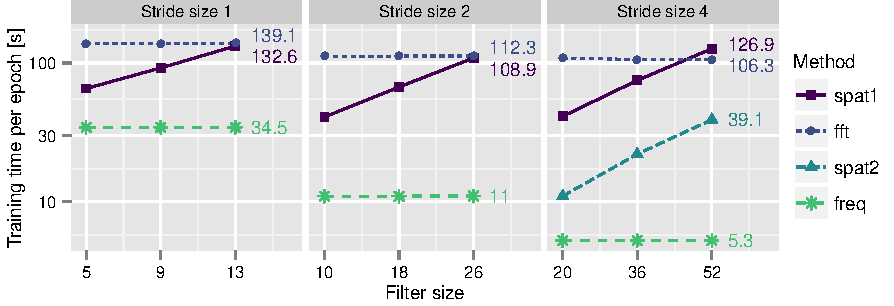
\includegraphics{figures/runtime_imgnet_c3}
%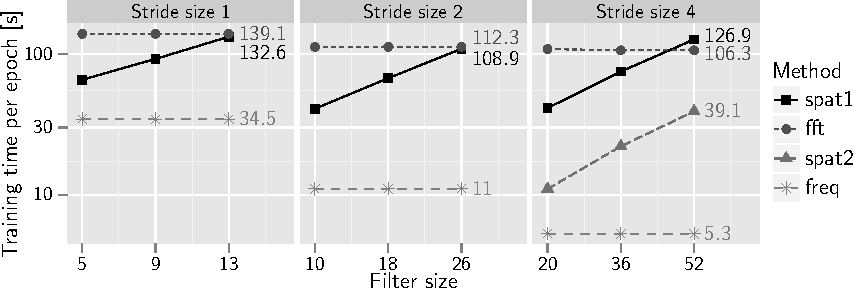
\includegraphics{figures/NECO-03-14-2099-Figure-2}
%\input{r_figures/runtime_imgnet_c3_bw}
}

\subfloat[Running times of training a second layer sconvRBM with
16, 32, and 64 channels (stride size 1).] {
\label{fig:run_imgnet_l2}
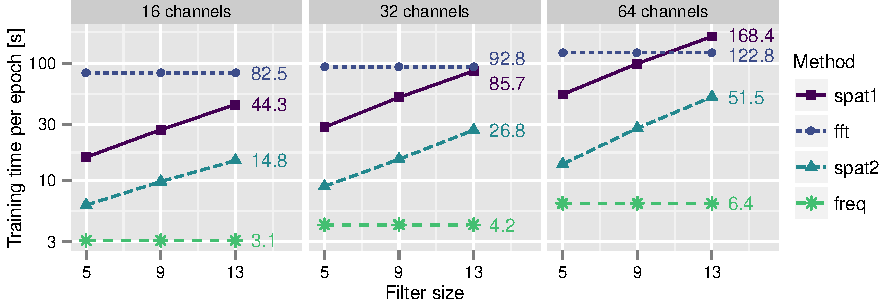
\includegraphics{figures/runtime_imgnet_c16-64}
%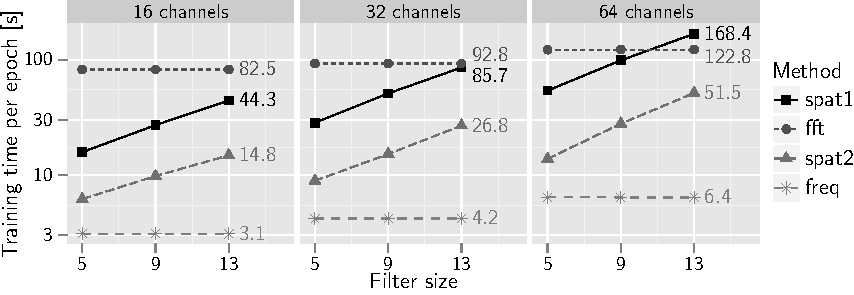
\includegraphics{figures/NECO-03-14-2099-Figure-3}
%\input{r_figures/runtime_imgnet_c16-64_bw}
}

\caption[Comparison of running times for training a sconvRBMs on 2D
images]{Comparison of running times for training a (a) first and (b) second
layer sconvRBM on 2D images using our frequency domain method (freq) and three
alternative methods using different convolution implementations: single image
convolutions (spat1), batched convolutions (spat2), and convolution by using
FFTs (fft). Due to internal limitations of the implementation of batched
convolutions, a comparison with spat2 could not be performed for images with a
resolution of \num{512x512} when using a stride size smaller than four.}
\label{fig:run_imgnet}
\end{figure}

\ref{fig:run_imgnet}\subref{fig:run_imgnet_l2} shows a similar comparison for
training the second convRBM layer for a stride size of one and varying filter
sizes and numbers of channels. In contrast to training the first layer, training
times mostly depend on the calculation of convolutions, where the impact of
calculating convolutions on the total running time increases with an increasing
number of channels. Training in the frequency domain is between 5 to 26 times
faster than training in the spatial domain using single-image convolutions, and
2 to 8 times faster than using batched convolutions. For all channel sizes,
batched training is about 3 to 4 times faster than non-batched training and
calculating convolutions using FFTs is much slower than batched training and
training in the frequency domain. To summarize, training of 2D images in the
frequency domain is much faster than training in the spatial domain even for
small filter sizes. Using the largest filter kernels in both layers, the
proposed method is shown to yield a speedup of 7 to 8 times compared to
state-of-the-art GPU implementations.

\subsubsection{Running Time Analysis on 3D Volumes (OASIS)}

\ref{fig:run_oasis} shows the comparison of running times for training a first
and second layer sconvRBM on 3D volumes for varying filter sizes, stride sizes,
and varying numbers of channels. In contrast to training on 2D images, the
computational costs of calculating 3D convolutions break even with calculating
FFTs even for small filter sizes, because the number of multiplications and
additions per convolution increases cubically, instead of quadratically, with
the filter kernel size. As a result, simply training by convolutions in the
frequency domain is faster than in the spatial domain. However, our proposed
training algorithm still outperforms both other methods, even at the smallest
filter size. For filter sizes of five and larger, our frequency domain
implementation is between 3.5 to 200 times faster than our spatial domain
implementation using single-image convolutions and 2.7 to 17 times faster than
calculating convolutions by FFTs. Similar to the results on 2D images, training
times of the first layer using a stride of one depend strongly on the time
required to calculate the expectation of the hidden units and to sample the
hidden units. Hence, performance improvements of our frequency domain method are
more pronounced for larger strides and numbers of channels, where the impact of
calculating convolutions on the total training time is also larger. This makes
the proposed method particularly suitable for training sconvRBMs on
high-resolution 3D volumes.

\begin{figure}[t!]
\subfloat[Running times of training a first layer sconvRBM with stride sizes of 1, 2, and 4.] {
\label{fig:run_oasis_l1}
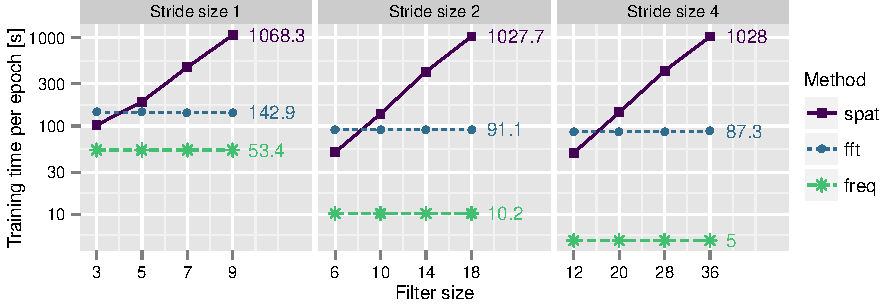
\includegraphics{figures/runtime_oasis_c1}
%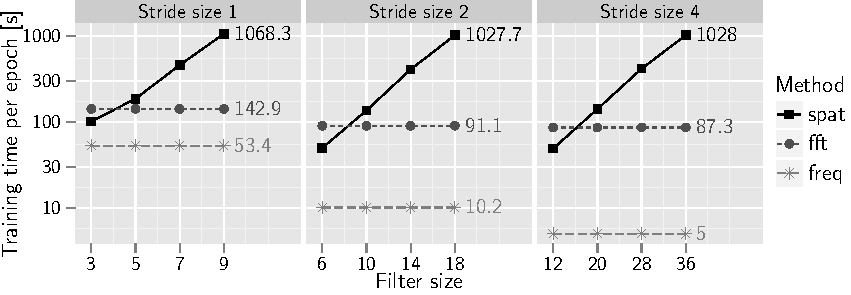
\includegraphics{figures/NECO-03-14-2099-Figure-4}
%\input{r_figures/runtime_oasis_c1_bw}
}

\subfloat[Running times of training a second layer sconvRBM with 8, 16, and 32
channels (stride size 1).] {
\label{fig:run_oasis_l2}
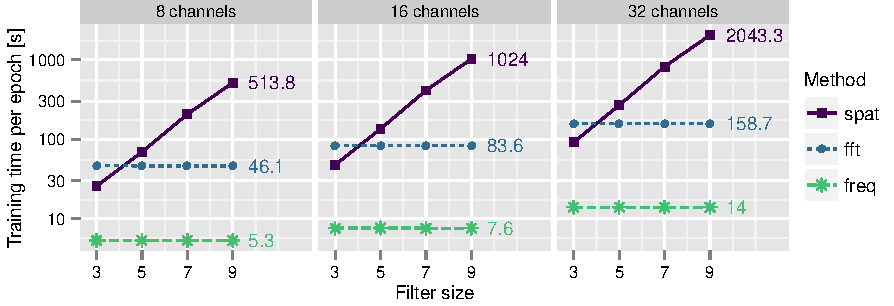
\includegraphics{figures/runtime_oasis_c8-32}
%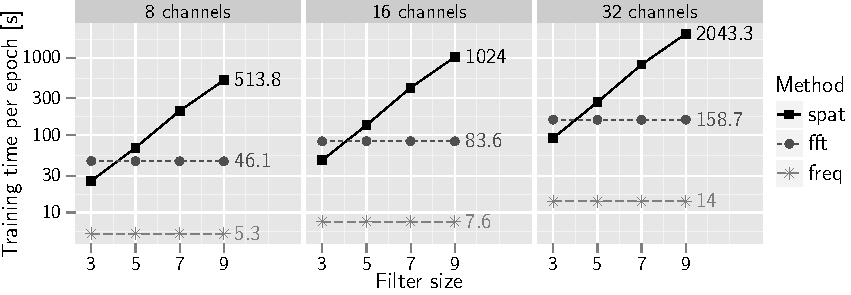
\includegraphics{figures/NECO-03-14-2099-Figure-5}
%\input{r_figures/runtime_oasis_c8-32_bw}
}
\caption[Comparison of running times for training a sconvRBMs on 3D
images]{Comparison of running times for training a (a) first and (b) second
layer sconvRBM on 3D volumes using a single 3D image convolution implementation
(spat), an implementation that calculates convolutions by using FFTs (fft), and
our proposed implementation in the frequency domain (freq).}
\label{fig:run_oasis}
\end{figure}

\subsection[Comparison of running times for calculating convolutions with
cuDNN]{Comparison of Running Times for Calculating Convolutions with cuDNN}

The \gls{cudnn} \citep{chetlur2014} is a GPU-accelerated library of primitives
that are commonly required to implement deep learning methods such as CNNs and
convDBNs. It is used internally by state-of-the-art deep learning frameworks
such as Caffe \citep{jia2014}, Theano \citep{bastien2012}, and Torch
\citep{collobert2011torch7}. The library provides highly optimized
implementations for calculating, e.g., batched 2D and 3D convolutions, pooling
operations, and different transfer functions. In this set of experiments, we
directly compared the time required to calculate convolutions when training a
CNN using our frequency domain implementation with cuDNN. We only consider
convolutions because they are the most time-consuming operations and because all
other operations are calculated in the same way. For the comparison with our
frequency domain implementation, the time measurements also include the time
required to calculate FFTs during the gradient calculation and for transforming
the accumulated gradient to spatial domain and back in order to trim the padded
filters to the original filter size. The parameters that we used for evaluating
the running time of different convolution implementations are summarized in
\ref{tab:cudnn_parameters}. The parameters represent typical values of the first
and second layer of a CNN, which are the layers that require the most time to
train, because the visible units of subsequent layers are commonly of much
smaller resolution. The key parameters that we varied are the image size, filter
size, and batch size. The hardware details of our test environment are
summarized in \ref{tab:cudnn_hardware}.

% TODO: explain training of CNNs: already have forward pass, but also need
% backwards pass and gradient calculation

% Experiments: - varying image size, batch size, filter size
%              - models used in this thesis (7-layer CEN, sconvDBN)
% Make this two subsubsections, one for detailed experiments and one for real
% models 
% Real models also show what reorganization does for you.
% Methods: frequency domain, frequency domain with padding, cuDNN
% Figure out what is common and what not.

\begin{table}
\centering
\caption{CNN layer parameters for the comparison with cuDNN.}
\label{tab:cudnn_parameters}
\begin{tabular}{cccccc}
\toprule
Experiment & \#Channels & Image size & Filter size & Filter count & Batch size
\\
\midrule
%\multirow{2}*{\minitab[c]{Varying\\ image size}} 
Varying & $2$  & $16^3, 17^3, \dotsc, 128^3$ & $9^3$ & $32$ & $8$ \\
image sizes & $32$ & $10^3, 11^3, \dotsc, 64^3$  & $9^3$ & $32$ & $8$ \\
\addlinespace
%\multirow{2}*{\minitab[c]{Varying\\ batch size}}
Varying & $2$  & $128^3$ & $9^3$ & $32$ & $1, 2, 4, 8$ \\
batch sizes & $32$ & $64^3$  & $9^3$ & $32$ & $1, 2, 4, 8$ \\
\addlinespace
%\multirow{2}*{\minitab[c]{Varying\\ filter size}}
Varying & $2$  & $128^3$ & $1^3, 2^3, \dotsc, 9^3$ & $32$ & $8$ \\
filter sizes & $32$ & $64^3$  & $1^3, 2^3, \dotsc, 9^3$ & $32$ & $8$ \\
\bottomrule
\end{tabular}
\end{table} 

\begin{table} 
\centering
\caption{Hardware specification of our test system for the comparison with
cuDNN.}
\label{tab:cudnn_hardware}
\begin{tabular} {ll}
\toprule
Processor & Intel i5-2500 CPU @ 3.30\,GHz \\
CPU Memory & 32\,GB \\
\addlinespace
Graphics Card & NVIDIA GeForce GTX 780 \\
GPU Cores & 2304 cores @ 0.94\,GHz \\
GPU Memory & 3\,GB \\
\bottomrule
\end{tabular}
\end{table}

\Ref{fig:imagesize} shows a comparison of the running times for calculating
convolutions using our frequency domain implementation and cuDNN for varying
image sizes. The FFT implementation that we used internally, cuFFT, is optimized
for image sizes that can be factorized as $2^a\times3^b\times5^c$. Therefore, we
also evaluated the time required to calculate convolutions when the input images
are automatically padded to a size for which cuFFT has been optimized. For image
sizes larger than $110^3$ voxels, cuFFT requires significantly more temporary
memory for calculating FFTs of unoptimized image sizes. Consequently, only the
running times of the padded frequency domain implementation and cuDNN were
measured for image sizes larger than $110^3$ voxels. Calculating convolutions in
the frequency domain scales better with an increase of the image size than
cuDNN. While cuDNN is the fastest method for very small image sizes, the padded
frequency domain implementation is more than 20 times faster for images with a
size of $128^3$ voxels and 2 input channels, and more than 18 times faster for
images with a size of $64^3$ voxels and 32 channels. Calculating the FFT and
therefore the running time of the frequency domain implementation varies
significantly depending on the input image size, and careful padding of the
input images is required to achieve consistently high performance.

% \begin{itemize}
% \item Improvements over cuDNN are larger for higher number of channels where the
% impact of calculating the FFT on the overall running time is also lower
% \item Going from 2 to 32 channels, the observed speed-up increases from
% approximately 10 times for the 2 channel comparison to approximately 18 times
% for the 32 channel comparison.
% \item Although the non-padded frequency domain implementation varies less for 32
% channels than for the 2 channel case, padding is still advantageous.
% \end{itemize}

\begin{figure}
\centering
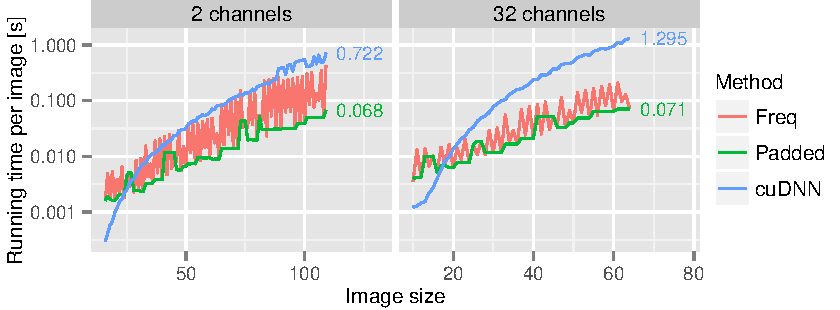
\includegraphics[width=0.95\textwidth]{figures/imagesize}
\caption[Comparison of running times of key operations for training a single
CNN layer.]{Comparison of running times of key operations for training a single
CNN layer for varying number of channels and input sizes. Frequency domain
training and training using cuDNN scales comparable for small numbers of
channels. For large numbers of channels, frequency domain method scales
slightly better to larger images.}
\label{fig:imagesize}
\end{figure}

\ref{tab:batchsize} shows a comparison of running times per image for varying
batch sizes and for varying number of channels. Increasing the batch size has
only a minor effect on the running time of cuDNN, while significantly increasing
the required amount of GPU memory. In contrast, the implementation in the
frequency domain does not require more memory, because each image of a
mini-batch is processed sequentially. Increasing the batch size reduces the
average running time per image of our frequency domain implementation, because
the FFTs required to trim the padded filters to the original filter size need to
be calculated only once per mini-batch, and have therefore a smaller impact on
the overall running time when the number of images per mini-batch is larger.

\begin{table}[tb]
\centering
\caption[Comparison of running times for calculating key operations for training
a CNN layer for different batch sizes]{Comparison of running times for
calculating key operations for training a CNN layer for different batch sizes.
Increasing the batch size reduces the impact of cropping the learned filters on
the overall running time and consequently reduces the average time to process
one image. The cuDNN implementation only benefits mildly from using larger
batches.}
\label{tab:batchsize}

\sisetup{
  round-mode = places,
  round-precision = 3,
  exponent-product = \cdot,
  detect-weight=true,
  detect-inline-weight=math,
  tight-spacing = false,
  table-align-text-post = false
}%
\begin{tabular}{
S[table-format=2.0]
S[table-format=1.3]
S[table-format=1.3]
S[table-format=1.3]
S[table-format=1.3]
S[table-format=1.3]
}
\toprule
{Batch size} & \multicolumn{4}{c}{Running time [s]} \\ 
& \multicolumn{2}{c}{$2$ channels} & \multicolumn{2}{c}{$32$
channels}
\\
           & {Freq} & {cuDNN} & {Freq} & {cuDNN} \\
\midrule
1   &  0.108588  & 1.39723 & 0.152864 & 1.31284 \\
2   &  0.0814377 & 1.01137 & 0.105898 & 1.30724 \\
4   &  0.0679075 & 1.24905 & 0.082375 & 1.30408 \\
8   &  0.0603056 & 1.24731 & 0.070710 & 1.29555 \\
%16  &  0.0568994 & {---}     & 0.064798 & 1.29431 \\
\bottomrule
\end{tabular}
\end{table}

The impact of the filter size on the running time is shown in
\ref{fig:filtersize}. For the first layer, training in the frequency domain is
faster for all filter sizes, where the speed-ups are larger for larger filters.
At a filter size of $9$, the speed-up is 20 times. For $32$ channels, cuDNN is
faster for very small filter sizes and training in the frequency domain breaks
even at a filter size of $3$. For filter sizes larger than $3$, training in the
frequency domain is substantially faster with a speed-up of up to $18$ times for
a filter size of $9$.

\begin{figure}
\centering
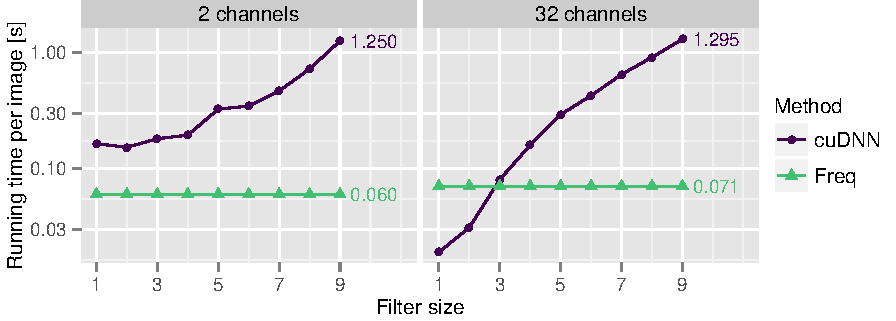
\includegraphics[width=0.9\textwidth]{figures/filtersize}
\caption[Comparison of running times of key operations for training a single
CNN layer.]{Comparison of running times of key operations for training a single
CNN layer for varying number of channels and filter sizes.}
\label{fig:filtersize}
\end{figure}

\ref{tab:usedmodels} shows a comparison of running times for calculating
convolutions of our frequency domain implementation with cuDNN for the 7-layer
\gls{cen} that we use in \ref{sec:segmentation} to segment \gls{ms} lesions, and
the first sconvRBM of the DBN model described in \ref{sec:manifold} to model the
variability in lesion distribution and brain morphology. For the 7-layer CEN,
the second convolutional and the first deconvolutional layer benefits the most
from training in the frequency domain due to the relatively large number of
channels in these layers. Overall, the convolutions required to train the
7-layer CEN can be calculated 6.3 times faster in the frequency domain compared
to cuDNN. In a second experiment, we compared the time required to directly
calculate strided convolutions with mapping strided convolutions to stride-1
convolutions by reorganizing the visible units of an sconvRBM. For the frequency
domain implementation, the direct method calculates stride-1 convolutions
instead of strided convolutions and discards the additional hidden units
afterwards, because strided convolutions cannot directly be calculated in the
frequency domain. Mapping strided convolutions to stride-1 convolutions speeds
up the training in the frequency domain by a factor of four compared to
calculating stride-1 convolutions in the frequency domain. Overall, calculating
the convolutions for training the first sconvRBM is 3.7 times faster using our
frequency domain implementation than the direct implementation of strided
convolutions of cuDNN.

\begin{table}
\caption[Comparison of running times of time critical operations of two example
deep learning models.]{Comparison of running times of time critical operations
of the 7-layer CEN-s used for segmenting lesions, and the first sconvRBM of
the lesion DBN using to model lesion distribution. The running times of pooling
layers we excluded.}
\label{tab:usedmodels}
\centering
\sisetup{
  round-mode = places,
  round-precision = 3,
  exponent-product = \cdot,
  detect-weight=true,
  detect-inline-weight=math,
  tight-spacing = false,
  table-align-text-post = false
}%

\begin{tabular}{l>{\raggedright}p{5cm}S[table-format=1.3]S[table-format=1.3]@{}S[table-format=2.3]}
\toprule
\multicolumn{2}{c}{Experiment} & \multicolumn{2}{c}{Running time
[s]\phantom{he}} & {Speed-up}
\\
& & {Freq} & {cuDNN} &  \\
\midrule
\multirow{5}*{\minitab[l]{$7$-layer CEN\\ used for lesion\\ segmentation}}
& 1st convolutional layer & 0.076582 & 0.498335 & 6.5072 \\
& 2nd convolutional layer & 0.0519153 & 0.523849 & 10.0904 \\
& 1st deconvolutional layer & 0.0519153 & 0.523849 & 10.0904 \\
& 2nd deconvolutional layer & 0.1477196 & 0.51716 & 3.500957 \\[0.5em]
& total & 0.3281322 & 2.063193 & 6.28768831587 \\
\midrule
\multirow{4}*{\minitab[l]{First sconvRBM of \\ the lesion DBN}}
& direct calculation of strided convolutions & 0.0755562 & 0.0683263 &
0.90431096323 \\
& strided convolutions mapped to stride-1 convolutions & 0.0186432 & 0.0705788 &
3.78576639204 \\
\bottomrule
\end{tabular}
\end{table}

\section{Conclusions}

We have presented a fast training method for convolutional models, which
performs training in the frequency domain in order to replace the time-consuming
computation of convolutions with simple element-wise multiplications. We have
shown that it is also essential to map the other operations to frequency space
wherever possible to minimize the number of Fourier transforms, and that this
greatly decreases training times over performing only the convolutions in the
frequency domain. In addition, our method can be efficiently implemented on the
GPU and is faster than a highly optimized GPU implementation of batched
convolutions in the spatial domain. We have evaluated the running time
improvements using two standard benchmark data sets, showing a speed-up of up to
8 times on 2D images from the ImageNet data set and up to 200 times on 3D
volumes from the OASIS data set. In addition, we have directly compared the time
required to calculate convolutions using our method with cuDNN, the current
state-of-the-art library for calculating 2D and 3D convolutions, with the
results showing that our method can calculate convolutions up to 20 times faster
than cuDNN.

% TODO: emphasize the key features compared to other FD implementations
% Only efficient when flipping can be expressed in the frequency domain
% otherwise either store flipped and non-flipped versions, which increases
% the amount of required memory, or requires flipped in spatial domain, which
% adds FFT calculations, or do it in batch-mode, which also increases memory

\chapter{White Matter Lesion Segmentation}
\label{sec:segmentation}

\section{Introduction}

Multiple sclerosis (MS) is an inflammatory and demyelinating disease of the
central nervous system with pathology that can be observed in vivo by magnetic
resonance imaging (MRI). MS is characterized by the formation of lesions,
primarily visible in the white matter on conventional MRI. Imaging biomarkers
based on the delineation of lesions, such as lesion load and lesion count, have
established their importance for assessing disease progression and treatment
effect. However, lesions vary greatly in size, shape, intensity and location,
which makes their automatic and accurate segmentation challenging.

\section{Related Work}

Many automatic methods have been proposed for the segmentation of MS
\mbox{lesions} over the last two decades \citep{garcia2013}, which can be
classified into unsupervised and supervised methods.

\subsection{Unsupervised Methods}

Unsupervised methods do not require a labeled data set for training. Instead,
lesions are identified as an outlier of, e.g., a subject-specific generative
model of tissue intensities
\citep{vanleemput2001,tomas2015,schmidt2012automated,roura2015}, or a generative
model of image patches representing a healthy population \citep{weiss2013}.
Alternatively, clustering methods have been used to segment healthy and lesion
tissue, where lesions are modelled as a separate tissue class
\citep{shiee2010topology,sudre2015}. In many methods, spatial priors of healthy
tissues are used to reduce false positives. For example, in addition to
modelling MS lesions as a separate intensity cluster, Lesion-TOADS
\citep{shiee2010topology} employs topological and statistical atlases to produce
a topology-preserving segmentation of all brain tissues.

To account for local changes of the tissue intensity distributions,
\citet{tomas2015} combined the subject-specific model of
the global intensity distributions with a voxel-specific model calculated from a
healthy population, where lesions are detected as outliers of the combined
model. A major challenge of unsupervised methods is that outliers are often not
specific to lesions and can also be caused by intensity inhomogeneities, partial
volume, imaging artifacts, and small anatomical structures such as blood
vessels, which leads to the generation of false positives. To overcome these
limitations, \citet{roura2015} employed an additional set of rules
to remove false positives, while \citet{schmidt2012automated} used
a conservative threshold for the initial detection of lesions, which are later
grown in a separate step to yield an accurate delineation.

\subsection{Supervised Methods}

Current supervised approaches typically start with a set of features, which can
range from small and simple to large and highly variable, and are either
predefined by the user \citep{geremia2010,guizard2015,subbanna2015} or gathered
in a feature extraction step such as by deep learning \citep{yoo2014}.
Voxel-based segmentation algorithms \citep{geremia2010,yoo2014} feed the
features and labels of each voxel into a general classification algorithm, such
as a random forest \citep{breiman2001}, to classify each voxel and to determine
which set of features are the most important for segmentation in the particular
domain. Voxel features and the labels of neighboring voxels can be incorporated
into Markov random field-based (MRF-based) approaches
\citep{subbanna2009,subbanna2015} to produce a spatially consistent
segmentation. As a strategy to reduce false positives, \citet{subbanna2015}
combined a voxel-level MRF with a regional MRF, which integrates a large set of
intensity and textural features extracted from the regions produced by the
voxel-level MRF with the labels of neighboring nodes of the regional MRF.
Library-based approaches leverage a library of pre-segmented images to carry out
the segmentation. For example, \citet{guizard2015} proposed a segmentation
method based on an extension of the non-local means algorithms
\citep{coupe2011}. The centers of patches at every voxel location are classified
based on matched patches from a library containing pre-segmented images, where
multiple matches are weighted using a similarity measure based on
rotation-invariant features.

\subsection{Patch-based Deep Learning Methods}

A recent breakthrough for the automatic segmentation using deep learning comes
from the domain of cell membrane segmentation, in which \citet{ciresan2012}
proposed classifying the centers of image patches directly using a convolutional
neural network (CNN) \citep{lecun1998} without a dedicated feature extraction
step. Instead, features are learned indirectly within the lower layers of the
neural network during training, while the higher layers can be regarded as
performing the classification, which allows the learning of features that are
specifically tuned to the segmentation task. However, the time required to train
patch-based methods can make the approach infeasible when the size and number of
patches are large.

\subsection{Fully Convolutional Methods}

Recently, different CNN architectures
\citep{long2015,ronneberger2015,brosch2015,kang2014fully} have been proposed
that are able to feed through entire images, which removes the need to select
representative patches, eliminates redundant calculations where patches overlap,
and therefore these models scale up more efficiently with image resolution.
\citet{kang2014fully} introduced the fully convolutional neural network (fCNN)
for the segmentation of crowds in surveillance videos. However, fCNNs produce
segmentations of lower resolution than the input images due to the successive
use of convolutional and pooling layers, both of which reduce the
dimensionality. To predict segmentations of the same resolution as the input
images, we recently proposed using a 3-layer convolutional encoder network (CEN)
\citep{brosch2015} for MS lesion segmentation. The combination of convolutional
\citep{lecun1998} and deconvolutional \citep{zeiler2011} layers allows our
network to produce segmentations that are of the same resolution as the input
images.

Another limitation of the traditional CNN is the trade-off between localization
accuracy, represented by lower-level features, and contextual information,
provided by higher-level features. To overcome this limitation, \citet{long2015}
proposed fusing the segmentations produced by the lower layers of the network
with the upsampled segmentations produced by higher layers. However, using only
low-level features was not sufficient to produce a good segmentation at the
lowest layers, which is why segmentation fusion was only performed for the three
highest layers. Instead of combining the segmentations produced at different
layers, \citet{ronneberger2015} proposed combining the features of different
layers to calculate the final segmentation directly at the lowest layer using an
11-layer u-shaped network architecture called u-net. Their network is composed
of a traditional contracting path (first half of the u), but augmented with an
expanding path (last half of the u), which replaces the pooling layers of the
contracting path with upsampling operations. To leverage both high- and
low-level features, shortcut connections are added between corresponding layers
of the two paths. However, upsampling cannot fully compensate for the loss of
resolution, and special handling of the border regions is still required.

% We have evaluated our method on two widely used publicly available data sets for
% the evaluation of MS lesion segmentation methods and a large in-house data set
% from an MS clinical trial, with a comparison of network architectures of
% different depths and with and without shortcuts\footnote{Where the risk of
% confusion is minimal, we will refer to the shortcut connections between two
% corresponding layers as a single shortcut (see Fig. 1).}.

\section{Methods}
\label{sec:method}

We propose a new convolutional network architecture that combines the advantages
of a CEN \citep{brosch2015} and a u-net \citep{ronneberger2015}. Our
network is divided into two pathways, a traditional convolutional pathway, which
consists of alternating convolutional and pooling layers, and a deconvolutional
pathway, which consists of alternating deconvolutional and unpooling layers and
predicts the final segmentation. Similar to the u-net, we introduce shortcut
connections between layers of the two pathways. In contrast to the u-net, our
network uses deconvolution instead of upsampling in the expanding pathway and
predicts segmentations that have the same resolution as the input images and
therefore does not require special handling of the border regions.

\begin{figure*}[tb]
\centering
\begin{tikzpicture}[
  node distance=0.75cm and 0.65cm,
  font=\footnotesize,
  conv/.style={green!60!black,-latex,thick},
  conv2/.style={green!60!black,latex-latex,thick},
  deconv/.style={-latex,blue!40!black,thick},
  %pooling/.style={-latex,red!60!black,thick,dashed},
  %unpooling/.style={-latex,brown!60!black,thick,dashed},
  pooling/.style={-latex,green!60!black,thick,dashed},
  unpooling/.style={-latex,blue!40!black,thick,dashed},
  channel/.style args={#1 and #2}{draw, fill=lightgray, inner sep=0pt,
      minimum width=#1, minimum height=#2}
]

% \tikzstyle{channel}=[draw,minimum width=64pt,fill=lightgray,inner
% sep=0pt,minimum height=#1]

% Network

\begin{scope}[local bounding box=network]
\node[channel=64pt and 3pt,pin=270:Input images] (inputs) {};
\node[channel=60pt and 16pt,above=of inputs] (clayer1) {};
\node[channel=30pt and 16pt,above=of clayer1] (pooling1) {};

\node[channel=64pt and 1pt,right=of inputs,pin=270:Segmentations] (outputs) {};
\node[channel=60pt and 16pt] (dlayer1) at (clayer1-|outputs) {};
\node[channel=30pt and 16pt,above=of dlayer1] (dpooling1) {};

\node[fit=(pooling1)(dpooling1),inner sep = 0pt] (pooling) {};
\node[channel=26pt and 16pt,above=of pooling] (clayer2) {};
\end{scope}

\draw[conv] (inputs)--node[left] {$w^{(1)}_\text{c}$} (clayer1);
\draw[pooling] (clayer1)--node[left] {} (pooling1);
\draw[conv] (pooling1)--node[left] {$w^{(3)}_\text{c}$} (clayer2);
\draw[deconv] (clayer2)--node[right=5pt] {$w^{(3)}_\text{d}$} (dpooling1);
\draw[unpooling] (dpooling1)--node[right] {} (dlayer1);
\draw[deconv] (dlayer1)--node[right] {$w^{(1)}_\text{d}$} (outputs);
\draw[deconv] (clayer1)--node[anchor=188,inner sep=10pt]
{$w^{(1)}_\text{s}$}(outputs);

% Part labels

\node[left=1pt of inputs] {$x^{(0)}$};
\node[left=1pt of clayer1] {$x^{(1)}$};
\node[left=1pt of pooling1] {$x^{(2)}$};
\node[left=1pt of clayer2] {$x^{(3)}$};

\node[right=1pt of outputs] {$y^{(0)}$};
\node[right=1pt of dlayer1] {$y^{(1)}$};
\node[right=1pt of dpooling1] {$y^{(2)}$};
\node[right=1pt of clayer2] {$y^{(3)}$};

% Layers

\draw[decorate,decoration={brace,raise=30pt}] (inputs.south west)
--node[left=35pt,align=center] (convl) {Convolutional\\ layer} (inputs.south
west|-clayer1.north west);

\draw[decorate,decoration={brace,raise=22pt}] (clayer1.south west)
--node[left=27pt,align=center] {Pooling\\ layer} (clayer1.south
west|-pooling1.north west);

\draw[decorate,decoration={brace,raise=25pt}] (pooling1.south west)
--node[left=30pt,align=center] {Convolutional\\ layer} (clayer2.north
west-|pooling1.south west);

\draw[decorate,decoration={brace,raise=30pt,mirror}] (outputs.south east)
--node[right=35pt,align=center] {Deconvolutional\\ layer with shortcut}
 (dlayer1.north east-|outputs.south east);

\draw[decorate,decoration={brace,raise=22pt,mirror}] (dlayer1.south east)
--node[right=27pt,align=center] {Unpooling\\ layer}
(dpooling1.north east-|dlayer1.south east);

\draw[decorate,decoration={brace,raise=25pt,mirror}] (dpooling1.south east)
--node[right=30pt,align=center] {Deconvolutional\\ layer}
(clayer2.north east-|dpooling1.south east);

% Legend

\begin{scope}[local bounding box=ghost,opacity=0]
\path[conv] node (conv) {convolution} [draw] (conv.west)
++(left:0.5)--++(right:0.5);

\path[pooling] node[right=0.8 of conv] (pool) {pooling} [draw] (pool.west)
++(left:0.5)--++(right:0.5);

\path[deconv] node[right=0.8 of pool] (dconv) {deconvolution} [draw]
(dconv.west) ++(left:0.5)--++(right:0.5);

\path[unpooling] node[right=0.8 of dconv] (unpool) {unpooling} [draw]
(unpool.west) ++(left:0.5)--++(right:0.5);
\end{scope}

\begin{scope}[local bounding box=ghost2,
    shift={($(network.south)-(ghost.north)$)},xshift=2pt,yshift=-7pt]

\path[conv] node (conv) {convolution} [draw] (conv.west)
++(left:0.5)--++(right:0.5);

\path[pooling] node[right=0.8 of conv] (pool) {pooling} [draw] (pool.west)
++(left:0.5)--++(right:0.5);

\path[deconv] node[right=0.8 of pool] (dconv) {deconvolution} [draw]
(dconv.west) ++(left:0.5)--++(right:0.5);

\path[unpooling] node[right=0.8 of dconv] (unpool) {unpooling} [draw]
(unpool.west) ++(left:0.5)--++(right:0.5);
\end{scope}

% Stack of CRBMs

\begin{scope}[local bounding box=dbn]
\node[channel=64pt and 3pt, left=6cm of inputs,pin=270:Input images] (rinputs)
{}; 
\node[channel=60pt and 16pt,above=of rinputs] (rclayer1) {};
\node[channel=30pt and 16pt,above=of rclayer1] (rpooling1) {};
\node[channel=26pt and 16pt,above=of rpooling1] (rclayer2) {};
\end{scope}

\draw[conv2] (rinputs)--node[left] {$\hat{w}^{(1)}$} (rclayer1);
\draw[pooling] (rclayer1)--node[right] {pooling} (rpooling1);
\draw[conv2] (rpooling1)--node[left] {$\hat{w}^{(2)}$} (rclayer2);

\node[left=1pt of rinputs] {$v^{(1)}$};
\node[left=1pt of rclayer1] {$h^{(1)}$};
\node[left=1pt of rpooling1] {$v^{(2)}$};
\node[left=1pt of rclayer2] {$h^{(2)}$};

\draw[decorate,decoration={brace,raise=5pt,mirror}] (rinputs.south east)
--node[right=10pt,align=center] (crbm) {convRBM$_1$} (rinputs.south
east|-rclayer1.north east);

\draw[decorate,decoration={brace,raise=5pt,mirror}] (rpooling1.south east)
--node[right=10pt,align=center] {convRBM$_2$} (rclayer2.north
east-|rpooling1.south east);

% \node[above=10pt of dbn,align=center] {Stack of Convolutional\\ Restricted
% Boltzmann Machines};
% \node[above=10pt of network] {Convolutional Encoder Network};

\node[above=15pt of dbn,align=center,font=\normalsize] {Pre-training};
\node[above=15pt of network,font=\normalsize] {Fine-tuning};

% \draw[->] (crbm.east|-dbn)-- node[above=2pt] {convert} 
% node[above,align=center]
% {$w_\text{c}^{(1)} = w^{(1)}$ \\
%  $w_\text{c}^{(2)} = w^{(2)}$ \\
%  $w_\text{d}^{(2)} = w^{(2)}$ \\
%  $w_\text{d}^{(1)} = 0.5w^{(1)}$ \\
%  $w_\text{s}^{(1)} = 0.5w^{(1)}$}
% (convl.west|-network);

%\draw (network.north west) rectangle (network.south east);
%\draw (ghost.north west) rectangle (ghost.south east);
%\draw (ghost2.north west) rectangle (ghost2.south east);

%\path[pooling] node (pool) at (-3,-1) {convolution};
%\draw[pooling] (conv.west) ++(left:0.5)--++(right:0.5);

%\draw[conv] (-3,-1)-- +(right:0.5) node[right] {convolution};
%\draw[pooling] (-0.5,-1)-- +(right:0.5) node[right] {pooling};
%\draw[deconv] (2,-1)-- +(right:0.5) node[right] {deconvolution};
%\draw[unpooling] (4.5,-1)-- +(right:0.5) node[right] {unpooling};

%\draw[pooling] (0,-1.5)-- +(right:0.5) node[right] {pooling};
%\draw[deconv] (0,-2)-- +(right:0.5) node[right] {deconvolution};
%\draw[unpooling] (0,-2.5)-- +(right:0.5) node[right] {unpooling};

\end{tikzpicture}

\caption[Pre-training and fine-tuning of the 7-layer convolutional encoder
network with shortcut that we used for our experiments]{Pre-training and
fine-tuning of the 7-layer convolutional encoder network with shortcut that we
used for our experiments. Pre-training is performed on the input images using a
stack of convolutional RBMs. The pre-trained weights and bias terms are used to
initialize a convolutional encoder network, which is fine-tuned on pairs of
input images, $x^{(0)}$, and segmentations, $y^{(0)}$.}

\label{fig:network}
\end{figure*}

\subsection{Segmentation as an Optimization Problem}

In this paper, the task of segmenting MS lesions is defined as finding a
function $s$ that maps multi-modal images $I$, e.g., $I = (I_\text{FLAIR},
I_\text{T1})$, to corresponding binary lesion masks $S$, where $1$ denotes a
lesion voxel and $0$ denotes a non-lesion voxel. Given a set of training images
$I_n$, $n \in \N$, and corresponding segmentations $S_n$, we model finding an
appropriate function for segmenting MS lesions as an optimization problem of the
following form
\begin{equation}
\hat{s} = \arg \min_{s \in \mathcal{S}} \sum_n E(S_n, s(I_n)),
\label{eq:segprob}
\end{equation}
where $\mathcal{S}$ is the set of possible segmentation functions, and $E$ is an
error measure that calculates the dissimilarity between ground truth
segmentations and predicted segmentations.

\subsection{Model Architecture}

The set of possible segmentation functions, $\mathcal{S}$, is modeled by the
convolutional encoder network with shortcut connections (CEN-s) illustrated in
\ref{fig:network}. A CEN-s is a type of convolutional neural network (CNN)
\citep{lecun1998} that is divided into two interconnected pathways, the
convolutional pathway and the deconvolutional \citep{zeiler2011} pathway. The
convolutional pathway consists of alternating convolutional and pooling layers.
The input layer of the convolutional pathway is composed of the image voxels
$x^{(0)}_i(\vect{p})$, $i \in [1, C]$, where $i$ indexes the modality or input
channel, $C$ is the number of modalities or channels, and $\vect{p} \in \N^3$
are the coordinates of a particular voxel. The convolutional layers
automatically learn a feature hierarchy from the input images. A convolutional
layer is a deterministic function of the following form
\begin{equation}
x^{(l)}_j = \max \Bigg(0, \sum_{i=1}^C\tilde{w}^{(l)}_{\text{c},ij}*x^{(l-1)}_i
+ b^{(l)}_j\Bigg),
\end{equation}
where $l$ is the index of a convolutional layer, $x^{(l)}_j$, $j \in [1,F]$,
denotes the feature map corresponding to the trainable convolution filter
$w^{(l)}_{\text{c},ij}$, $F$ is the number of filters of the current layer,
$b^{(l)}_j$ are trainable bias terms, $*$ denotes valid convolution, and
$\tilde{w}$ denotes a flipped version of $w$, i.e., $\tilde{w}(a) = w(-a)$. To
be consistent with the inference rules of convolutional restricted Boltzmann
machines (convRBMs) \citep{lee2009convolutional}, which are used for
pre-training, convolutional layers convolve the input signal with flipped filter
kernels, while deconvolutional layers calculate convolutions with non-flipped
filter kernels. We use rectified linear units \citep{nair2010} in all layers
except for the output layers, which have shown to improve the classification
performance of CNNs \citep{krizhevsky2012}. A convolutional layer is followed by
an average pooling layer \citep{scherer2010evaluation} that halves the number of
units in each dimension by calculating the average of each block of \num{2x2x2}
units per channel.

The deconvolutional pathway consists of alternating deconvolutional and
unpooling layers with shortcut connections to the corresponding
convolutional layers. The first deconvolutional layer uses the extracted
features of the convolutional pathway to calculate abstract segmentation
features
\begin{equation}
y^{(L-1)}_i = \max\Bigg(0, \sum_{j=1}^Fw^{(L)}_{\text{d},ij}\circledast
y^{(L)}_j + c^{(L-1)}_{i}\Bigg),
\end{equation}
where $y^{(L)} = x^{(L)}$, $L$ denotes the number of layers of the convolutional
pathway, $w^{(L)}_{\text{d},ij}$ and $c^{(L-1)}_i$ are trainable parameters of
the deconvolutional layer, and $\circledast$ denotes full convolution. To be
consistent with the general notation of deconvolutions \citep{zeiler2011}, the
non-flipped version of $w$ is convolved with the input signal.

Subsequent deconvolutional layers use the activations of the previous layer and
corresponding convolutional layer to calculate more localized segmentation
features
\begin{equation}
y^{(l)}_i = \max\Bigg(0, 
\sum_{j=1}^Fw^{(l+1)}_{\text{d},ij}\circledast y^{(l+1)}_j
+ \sum_{j=1}^F w^{(l+1)}_{\text{s},ij}\circledast x^{(l+1)}_j +
c^{(l)}_i\Bigg),
\end{equation}
where $l$ is the index of a deconvolutional layer with shortcut, and
$w^{(l+1)}_{\text{s},ij}$ are the shortcut filter kernels connecting the
activations of the convolutional pathway with the activations of the
deconvolutional pathway. The last deconvolutional layer integrates the low-level
features extracted by the first convolutional layer with the high-level features
from the previous layer to calculate a probabilistic lesion mask
\begin{equation}
y^{(0)}_1 = \sigm\Bigg(\sum_{j=1}^F\Big(w^{(1)}_{\text{d},1j}\circledast
y^{(1)}_j +
w^{(1)}_{\text{s},1j}\circledast x^{(1)}_j\Big) + c^{(0)}_1\Bigg),
\end{equation}
where we use the sigmoid function defined as $\sigm(z) = (1 + \exp(-z))^{-1}, z
\in \R$ instead of the rectified linear function in order to obtain a
probabilistic segmentation with values in the range between 0 and 1.
To produce a binary lesion mask from the probabilistic output of our model, we
chose a fixed threshold such that the mean Dice similarity coefficient
\citep{dice1945measures} is maximized on the training set and used the same
threshold for the evaluation on the test set.

\subsection{Gradient Calculation}

The parameters of the model can be efficiently learned by minimizing the error
$E$ for each sample of the training set, which requires the calculation of the
gradient of $E$ with respect to the model parameters \citep{lecun1998}.
Typically, neural networks are trained by minimizing the sum of squared
differences (SSD), which can be calculated for a single image as follows
\begin{equation}
% Error function
E = \frac{1}{2}\sum_{\vect{p}}\left(S(\vect{p}) -
y^{(0)}(\vect{p})\right)^2,
\end{equation}
where $\vect{p} \in \N^3$ are the coordinates of a particular voxel.
The partial derivatives of the error with respect to the model parameters can be
calculated using the delta rule and are given by 
\begin{align}
\label{eq:dEd}
% Deconvolutional filters
\frac{\partial E}{\partial w^{(l)}_{\text{d},ij}} &=
\delta^{(l-1)}_{\text{d},i} * \tilde{y}^{(l)}_j, &
% Deconvolutional bias
\frac{\partial E}{\partial c^{(l)}_i} &= \sum_{\vect{p}}
\delta^{(l)}_{\text{d},i}(\vect{p}), \\
\label{eq:dEs}
% Shortcut filters
\frac{\partial E}{\partial w^{(l)}_{\text{s},ij}}
 &= \delta^{(l-1)}_{\text{d},i} * \tilde{x}^{(l)}_j, \\
 \label{eq:dEc}
% Convolutional filters
\frac{\partial E}{\partial w^{(l)}_{\text{c},ij}} 
&= x^{(l-1)}_i * \tilde{\delta}^{(l)}_{\text{c},j},\text{ and}&
% Convolutional bias
\frac{\partial E}{\partial b^{(l)}_i} &= \sum_{\vect{p}}
\delta^{(l)}_{\text{c},i}(\vect{p}).
\end{align}
For the first layer, $\delta^{(0)}_{\text{d},1}$ can be calculated by
\begin{equation}
% Delta update
\delta^{(0)}_{\text{d},1} = \big(y^{(0)}_1
-S\big)y^{(0)}_1\big(1-y^{(0)}_1\big).
\label{eq:delta0}
\end{equation}
The derivatives of the error with respect to the parameters of the other layers
can be calculated by applying the chain rule of partial derivatives, which
yields to
\begin{align}
\label{eq:deltad}
% Delta update of deconvolutional layer
\delta^{(l)}_{\text{d},j} &=
\big(\tilde{w}^{(l)}_{\text{d},ij}*\delta^{(l-1)}_{\text{d},i}\big)\I\big(y^{(l)}_j
> 0\big),\\
\label{eq:deltac}
% Delta update of convolutional layer
\delta^{(l)}_{\text{c},i} &=
\big(w^{(l+1)}_{\text{c},ij}\circledast\delta^{(l+1)}_{\text{c},j}\big)\I\big(x^{(l)}_i
> 0\big),
\end{align}
where $l$ is the index of a deconvolutional or convolutional layer,
$\delta^{(L)}_{\text{c},i} = \delta^{(L)}_{\text{d},j}$, and $\I(z)$ denotes the
indicator function defined as $1$ if the predicate $z$ is true and $0$
otherwise. If a layer is connected through a shortcut,
$\delta^{(l)}_{\text{c},j}$ needs to be adjusted by propagating the error back
through the shortcut connection. In this case, $\delta^{(l)}_{\text{c},j}$ is
calculated by
\begin{equation}
% Delta update convolutional with shortcut
\delta^{(l)}_{\text{c},j} =
\big(\delta^{(l)}_{\text{c},j}{}'+
\tilde{w}^{(l)}_{\text{s},ij}*\delta^{(l-1)}_{\text{d},i}\big)\I\big(x^{(l)}_j
> 0\big),
\label{eq:deltas}
\end{equation}
where $\delta^{(l)}_{\text{c},j}{}'$ denotes the activation of unit
$\delta^{(l)}_{\text{c},j}$ before taking the shortcut connection into account.

The sum of squared differences is a good measure of classification accuracy, if
the two classes are fairly balanced. However, if one class contains vastly more
samples, as is the case for lesion segmentation, the error measure is dominated
by the majority class and consequently, the neural network would learn to ignore
the minority class. To overcome this problem, we use a combination of
sensitivity and specificity, which can be used together to measure
classification performance even for vastly unbalanced problems. More precisely,
the final error measure is a weighted sum of the mean squared difference of the
lesion voxels (sensitivity) and non-lesion voxels (specificity), reformulated to
be error terms:
\begin{equation} 
E = r\frac{\textstyle\sum_{\vect{p}} \left(S(\vect{p}) -
y^{(0)}(\vect{p})\right)^2 S(\vect{p})}{\textstyle\sum_{\vect{p}} S(\vect{p})}
 + (1-r)\frac{\textstyle\sum_{\vect{p}} \left(S(\vect{p}) -
y^{(0)}(\vect{p})\right)^2 \big(1 - S(\vect{p})\big)}{%
\textstyle\sum_{\vect{p}}\big(1 - S(\vect{p})\big)}.
\end{equation}
We formulate the sensitivity and specificity errors as squared errors in order
to yield smooth gradients, which makes the optimization more robust. The
sensitivity ratio $r$ can be used to assign different weights to the two terms.
Due to the large number of non-lesion voxels, weighting the specificity error
higher is important, but based on preliminary experimental results \cite{brosch2015},
the algorithm is stable with respect to changes in $r$, which largely affects the
threshold used to binarize the probabilistic output. A detailed evaluation of
the impact of the sensitivity ratio on the learned model is presented in
\ref{sec:trainparams}.

To train our model, we must compute the derivatives of the modified objective
function with respect to the model parameters. Equations
\ref{eq:dEd}--\ref{eq:dEc} and \ref{eq:deltad}--\ref{eq:deltas} are a
consequence of the chain rule and independent of the chosen similarity measure.
Hence, we only need to derive the update rule for $\delta^{(0)}_{\text{d},1}$.
With $\alpha = 2r (\sum_{\vect{p}}S(\vect{p}))^{-1}$ and $\beta = 2(1 -
r)(\sum_{\vect{p}}(1 - S(\vect{p})))^{-1}$, we can rewrite $E$ as
\begin{align}
E=& \frac{1}{2}\sum_{\vect{p}}\left(S(\vect{p}) - y^{(0)}(\vect{p})\right)^2
\alpha S(\vect{p}) +
\frac{1}{2}\sum_{\vect{p}}\left(S(\vect{p})-y^{(0)}(\vect{p})\right)^2
\beta\big(1-S(\vect{p})\big)\\
=& \frac{1}{2}\sum_{\vect{p}}\big(\alpha S(\vect{p}) +
\beta(1-S(\vect{p}))\big)\Big(S(\vect{p})-y^{(0)}_1(\vect{p})\Big)^2.
\end{align}
Our objective function is similar to the SSD, with an additional multiplicative
term applied to the squared differences. The additional factor is constant with
respect to the model parameters. Consequently, $\delta^{(0)}_{\text{d},1}$ can
be derived analogously to the SSD case, and the new factor is simply carried
over:
\begin{equation} 
\delta^{(0)}_{\text{d},1} = \big(\alpha S + \beta (1 - S)\big)\big(y^{(0)}_1 -
S\big) y^{(0)}_1 \big(1 - y^{(0)}_1\big).
\end{equation}

\subsection{Training}

At the beginning of the training procedure, the model parameters need to be
initialized and the choice of the initial parameters can have a big impact on
the learned model \citep{sutskever2013importance}. In our experiments, we found
that initializing the model using pre-training \citep{hinton2006} on the input
images was required in order to be able to fine-tune the model using the ground
truth segmentations without getting stuck early in a local minimum. Pre-training
can be performed layer by layer \citep{hinton2006b} using a stack of convRBMs
(see \ref{fig:network}), thereby avoiding the potential problem of
vanishing or exploding gradients \citep{hochreiter1991untersuchungen}. The first
convRBM is trained on the input images, while subsequent convRBMs are trained on
the hidden activations of the previous convRBM. After all convRBMs have been
trained, the model parameters of the CEN-s can be initialized as follows
(showing the first convolutional and the last deconvolutional layers only, see
\ref{fig:network})

\begin{align}
w_{\text{c}}^{(1)} &= \hat{w}^{(1)}, &
w_{\text{d}}^{(1)} &= 0.5\hat{w}^{(1)}, &
w_{\text{s}}^{(1)} &= 0.5\hat{w}^{(1)} \\
b^{(1)} &= \hat{b}^{(1)}, &
c^{(0)} &= \hat{c}^{(1)},
\end{align}
where $\hat{w}^{(1)}$ are the filter weights, $\hat{b}^{(1)}$ are the hidden
bias terms, and $\hat{c}^{(1)}$ are the visible bias terms of the first convRBM.

A major challenge for gradient-based optimization methods is the choice of an
appropriate learning rate. Classic stochastic gradient descent \citep{lecun1998}
uses a fixed or decaying learning rate, which is the same for all parameters of
the model. However, the partial derivatives of parameters of different layers
can vary substantially in magnitude, which can require different learning rates.
In recent years, there has been an increasing interest in developing methods for
automatically choosing independent learning rates. Most methods (e.g., AdaGrad
by \citealp{duchi2011adaptive}; AdaDelta by \citealp{zeiler2012adadelta};
RMSprop by \citealp{dauphin2015rmsprop}; and Adam by \citealp{kingma2014adam})
collect different statistics of the partial derivatives over multiple iterations
and use this information to set an adaptive learning rate for each parameter.
This is especially important for the training of deep networks, where the
optimal learning rates often differ greatly for each layer. In our initial
experiments, networks obtained by training with AdaDelta, RMSprop, and Adam
performed comparably well, but AdaDelta was the most robust to the choice of
hyperparameters, so we used AdaDelta for all results reported.

\subsection{Implementation}

% TODO: Implementation outlined in a previous section

Pre-training and fine-tuning were performed using the highly optimized
GPU-accelerated implementation of 3D convRBMs and CENs explained in
\ref{sec:training}. Our frequency domain
implementation significantly speeds up the training by mapping the calculation
of convolutions to simple element-wise multiplications, while adding only a
small number of Fourier transforms. This is especially beneficial for the
training on 3D volumes, due to the increased number of weights of 3D kernels
compared to 2D. Although GPU-accelerated deep learning libraries based on cuDNN
\citep{chetlur2014} are publicly available (e.g.,
\citealp{jia2014,bastien2012,collobert2011torch7}), we trained our models using
our own implementation, because we have found that it performs the most
computationally intensive training operations 6 times faster than cuDNN in a
direct comparison (see \ref{tab:usedmodels} on page \pageref{tab:usedmodels}).
 
\sisetup{separate-uncertainty=true,detect-weight=true,detect-inline-weight=math}

\section{Experiments and Results}

We evaluated our method on two publicly available data sets (from the MICCAI
2008 MS lesion segmentation
challenge\footnote{\url{http://www.ia.unc.edu/MSseg/}} and the ISBI 2015
longitudinal MS lesion segmentation
challenge\footnote{\url{http://iacl.ece.jhu.edu/MSChallenge}}), which allows for
a direct comparison with many state-of-the-art methods. In addition, we have
used a much larger data set containing four different MRI sequences from a
multi-center clinical trial in relapsing remitting MS, which tends to have the
most heterogeneity among the MS subtypes. This data test is challenging due to
the large variability in lesion size, shape, location, and intensity as well as
varying contrasts produced by different scanners. The clinical trial data set
was used to carry out a detailed analysis of different CEN architectures using
different combinations of modalities, with a comparison to five publicly
available state-of-the-art methods.

\subsection{Data Sets and Pre-processing}

\subsubsection{Public data sets}
The data set of the MICCAI 2008 MS lesion segmentation challenge
\citep{styner20083d} consists of 43 T1-weighted (T1w), T2-weighted (T2w), and
FLAIR MRIs, divided into 20 training cases for which ground truth segmentations
are made publicly available, and 23 test cases. In a first experiment, we
evaluated our method on the 20 training cases using 5-fold cross-validation. In
a second experiment, we trained our model on the 20 training cases and then used
the trained model to segment the 23 test cases, which were sent to the challenge
organizers for independent evaluation.

The data set of the ISBI 2015 longitudinal MS lesion segmentation challenge
consists of 21 visit sets, each with T1w, T2w, proton density-weighted (PDw),
and FLAIR MRIs. The challenge was not open for new submissions at the time of
writing this article. Therefore, we evaluated our method on the training set
using leave-one-subject-out cross-validation, following the evaluation protocol
of the second place method by \cite{jesson2015} and third place method by
\cite{maier2015} from the challenge proceedings. The paper of the first place
method does not have sufficient details to replicate their evaluation.

\subsubsection{Clinical trial data set}

We used two different clinical trial data sets to evaluate our method. The first
data set contains images of 500 subjects split equally into training and test
sets. The images were acquired from 45 different scanning sites. For each
subject, the data set contains T2- and PD-weighted MRIs with a voxel size of
\SI{0.937x0.937x3.000}{\milli\metre}. The main preprocessing steps included
rigid intra-subject registration, brain extraction, intensity normalization, and
background cropping. This data set was used to evaluate how many images are
required to train a simple 3-layer CEN without overfitting. Training on a
single GeForce GTX 780 graphics card took between 6 and 32 hours per model
depending on the training set size. However, once the network is trained,
segmentation of new images can be performed in less than one second.

The second data set was collected from 67 different scanning sites using
different 1.5\,T and 3\,T scanners, and consists of T1w, T2w, PDw, and FLAIR
MRIs from 195 subjects, most with two time points (377 visit sets in total). In
contrast to the previous data set, this data set also contains T1w and FLAIR
MRIs, which allows for a direct comparison with other competing methods, which
require these modalities. The image dimensions and voxel sizes vary by site, but
most of the T1w images have close to \SI{1}{\milli\meter} isotropic voxels,
while the other images have voxel sizes close \SI{1x1x3}{\milli\meter}. All
images were skull-stripped using the brain extraction tool (BET)
\citep{jenkinson2005bet2}, followed by an intensity normalization to the
interval $[0,1]$, and a 6 degree-of-freedom intra-subject registration using one
of the \SI{3}{\milli\meter} scans as the target image to align the different
modalities. To speed-up the training, all images were cropped to a
\num{164x206x52} voxel subvolume with the brain roughly centered. The ground
truth segmentations for both data sets were produced using an existing
semiautomatic 2D region-growing technique, which has been used successfully in a
number of large MS clinical trials (e.g.,
\citealp{kappos2006long,traboulsee2008reduction}).
Each lesion was manually identified by an experienced radiologist and then
interactively grown from the seed point by a trained technician.

We divided the data set into a training ($n=250$), validation ($n=50$), and test
set ($n=77$) such that images of each set were acquired from different scanning
sites. The training, validation, and test sets were used for training our
models, for monitoring the training progress, and to evaluate performance,
respectively. The training set was also used to perform parameter tuning of the
other methods used for comparison. Pre-training and fine-tuning of our 7-layer
CEN-s took approximately 27 hours and 37 hours, respectively, on a single
GeForce GTX 780 graphics card. Once the network is trained, new multi-contrast
images can be segmented in less than one second.

\subsection{Comparison to Other Methods}
\label{sec:othermethods}

We compared our method with the five publicly available methods, some of which
are widely used for clinical research and are established in the literature
(e.g., \citealp{sudre2015,subbanna2015,guizard2015}) as reference points for
comparison. These five methods include:
\begin{enumerate}
\item Expectation maximization segmentation (EMS) method \citep{vanleemput2001};
\item Lesion growth algorithm (LST-LGA) \citep{schmidt2012automated}, as
implemented in the Lesion Segmentation Toolbox (LST) version 2.0.11;
\item Lesion prediction algorithm (LST-LPA) also implemented in the same LST toolbox;
\item Lesion-TOADS version 1.9 R \citep{shiee2010topology}; and 
\item Salem Lesion Segmentation (SLS) toolbox \citep{roura2015}.
\end{enumerate}
The Lesion-TOADS software only takes T1w and FLAIR MRIs and has no tunable
parameters, so we used the default parameters to carry out the segmentations.
The performance of EMS depends on the choice of the Mahalanobis distance
$\kappa$, the threshold $t$ used to binarize the probabilistic segmentation, and
the modalities used. We applied EMS to segment lesions using two combinations of
modalities: a) T1w, T2w, and PDw, as used in the original paper
\citep{vanleemput2001}, and b) all four available modalities (T1w, T2w, PD2,
FLAIR). We compared the segmentations produced for all combinations of $\kappa =
2.0, 2.2, \dotsc, 4.6$ and $t = 0.05, 0.10, \dotsc, 1.00$ with the ground truth
segmentations on the training set and chose the values that maximized the
average DSC ($\kappa = 2.6, t = 0.75$ for three modalities; $\kappa = 2.8, t =
0.9$ for four modalities).

The LST-LGA and LST-LPA of the LST toolbox only take T1w and FLAIR MRIs as
input, and we used those modalities to tune the initial threshold $\kappa$ of
LST-LGA for $\kappa = 0.05, 0.10, \dotsc, 1.00$ and the threshold $t$ used by
LST-LPA to binarize the probabilistic segmentations for $t = 0.05, 0.10, \dotsc,
1.00$. The optimal parameters were $\kappa = 0.10$ and $t = 0.45$, respectively.

Similarly, the SLS toolbox, which is the most recently published work
\citep{roura2015} also only takes T1w and FLAIR MRIs as input. This method uses
an initial brain tissue segmentation obtained from the T1w images and segments
lesions by treating lesional pixels as outliers to the normal appearing GM brain
tissue on the FLAIR images. This method has three key parameters:
$\omega_\text{nb}$, $\omega_\text{ts}$, and $\alpha_\text{sls}$. We tuned these
parameters on the training set via a grid-search over a range of values as
suggested by \citet{roura2015}.

\subsection{Measures of Segmentation Accuracy}
 
We used the following six measures to produce a comprehensive evaluation
of segmentation accuracy as there is generally no single measure that is
sufficient to capture all information relevant to the quality of a produced
segmentation \citep{garcia2013review}.

The first measure is the Dice similarity coefficient (DSC)
\cite{dice1945measures} that computes a normalized overlap value between the
produced and ground truth segmentations, and is defined as
\begin{equation}
\text{DSC} = \frac{2 \times \text{TP}}{2 \times \text{TP} + \text{FP} +
\text{FN}},
\end{equation}
where TP, FP, and FN denote the number of true positive, false positive, and
false negative voxels, respectively. A value of \SI{100}{\percent} indicates a
perfect overlap of the produced segmentation and the ground truth.
The DSC incorporates measures of over- and underestimation into a single metric,
which makes it a suitable measure to compare overall segmentation accuracy. In
addition, we have used the true positive rate (TPR) and the positive predictive
value (PPV) to provide further information on specific aspects of segmentation
performance. The TPR is used to measure the fraction of the lesion regions in
the ground truth that are correctly identified by an automatic method. It is
defined as
\begin{equation}
\text{TPR} = \frac{\text{TP}}{\text{TP} + \text{FN}},
\end{equation}
where a value of \SI{100}{\percent} indicates that all true lesion voxels are
correctly identified. The PPV is used to determine the extent of
the regions falsely classified as lesion by an automatic method.
It is defined as the fraction of true lesion voxels out of all
identified lesion voxels
\begin{equation}
\text{PPV} = \frac{\text{TP}}{\text{TP} + \text{FP}},
\end{equation}
where a value of \SI{100}{\percent} indicates that all voxels that are
classified as lesion voxels are indeed lesion voxels as defined by the ground
truth (no false positives).

We also measured the relative absolute volume difference between the
ground truth and the produced segmentation by computing their volumes
($\text{\textit{Vol}}$), i.e.,
\begin{equation}
\text{VD} = \frac{\text{\textit{Vol}}(\text{\textit{Seg}}) -
                    \text{\textit{ Vol}}(\text{\textit{GT}})}
                {\text{\textit{ Vol}}(\text{\textit{GT}})},
\end{equation}
where $Seg$ and $GT$ denote the obtained segmentation and ground truth,
respectively. However, it has been noted \cite{garcia2013review} that wide
variability exists even between the lesion segmentations of trained experts, and
thus, the achieved volume differences reported in the literature have ranged
from \SI{10}{\percent} to \SI{68}{\percent}.

For more precise evaluation, we have also included the lesion-wise true positive
rate (LTPR) and the lesion-wise false positive rate (LFPR) that are much more
sensitive in measuring the segmentation accuracy of smaller lesions, which are
important to detect when performing early disease diagnosis
\cite{garcia2013review}.
More specifically, the LTPR measures the true positive rate (TPR) on a per
lesion-basis and is defined as
\begin{equation}
\text{LTPR} = \frac{\text{LTP}}{\text{\#RL}},
\end{equation}
where LTP denotes the number of lesion true positive, i.e., the number
lesions in the reference segmentation that overlap with a lesion in the produced
segmentation, and \#RL denotes the total number of lesions in the reference
segmentation. An LTPR with a value of \SI{100}{\percent} indicates that all
lesions are correctly identified. Similarly, the lesion-wise false positive rate
(FPR) measures the fraction of the segmented lesions that are not in the ground
truth and is defined as
\begin{equation}
\text{LFPR} = \frac{\text{LFP}}{\text{\#PL}},
\end{equation}
where LFP denotes the number of lesion false positives, i.e., the number of
lesions in the produced segmentation that do not overlap with a lesion in the
reference segmentation, and \#PL denotes the total number of lesions in the
produced segmentation. An LFPR with a value of \SI{0}{\percent} indicates that
no lesions were incorrectly identified.

\begin{figure}[tb]
\centering
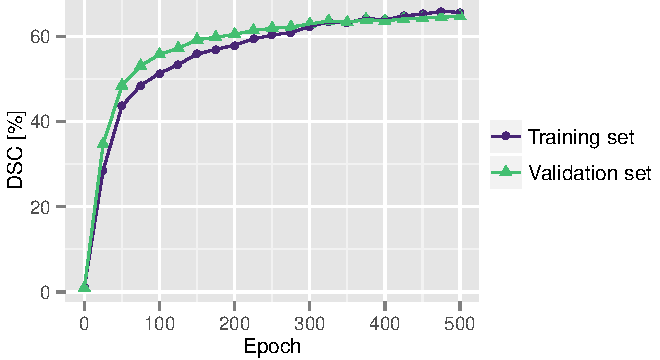
\includegraphics[width=0.7\textwidth]{figures/tmi/ems_progress}
\caption[Improvement in the mean DSC computed on the training and test sets
during training]{Improvement in the mean DSC computed on the training and test
sets during training. Only small improvements can be observed after 400 epochs.}
\label{fig:epochs}
\end{figure}

\subsection{Training Parameters}
\label{sec:trainparams}

The most influential parameters of the training method are the number of epochs
and the sensitivity ratio. \ref{fig:epochs} shows the mean DSC evaluated on
the training and validation sets of the second clinical data set as computed
during training of a \mbox{7-layer} CEN-s up to 500 epochs.
The mean DSC scores increase monotonically, but the improvements are minor after
400 epochs. The optimal number of epochs is a trade-off between accuracy and
time required for training. Due to the relatively small improvements after 400
epochs, we decided to stop the training procedure at 500 epochs. For the
challenge data sets, due to their small sizes, we did not employ a subset of the
data for a dedicated validation set to choose the number of epochs. Instead, we
set the number of epochs to 2500, which corresponds to roughly the same number
of gradient updates compared to the clinical trial data set.

\begin{figure}[tb]
\centering
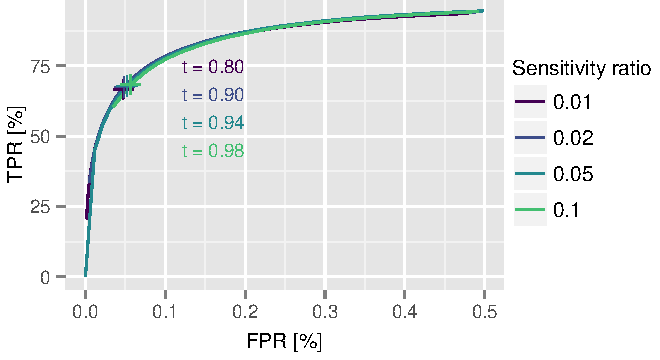
\includegraphics[width=0.7\textwidth]{figures/tmi/roc2}
\caption[ROC curves for different sensitivity ratios $r$]{ROC curves for
different sensitivity ratios $r$. A `$+$' marks the TPR and FPR of the optimal
threshold. Varying the value of $r$ results in almost identical ROC curves and
only causes a change of the optimal threshold $t$, which shows the robustness of
our method with respect to the sensitivity ratio.}
\label{fig:ratio}
\end{figure}

To determine an effective sensitivity ratio, we measured the performance on the
validation set over a range of values. For each choice of ratio, we binarized
the segmentations using a threshold that maximized the DSC on the training set.
\ref{fig:ratio} shows a set of ROC curves for different choices of the
sensitivity ratio ranging from 0.01 to 0.10 and the corresponding optimal
thresholds. The plots illustrate our findings that our method is not sensitive
to the choice of the sensitivity ratio, which mostly affects the optimal
threshold. We chose a fixed sensitivity ratio of 0.02 for all our experiments.


\subsection{Impact of the Training Set Size on the Segmentation Performance}

To evaluate the impact of the training set size on the segmentation performance,
we trained a CEN with 3 layers on the first in-house data set with a varying
number of training samples and calculated the mean DSC on the training and test
sets as illustrated in \ref{fig:bioms}. For small training sets, there is a
large difference between the DSCs on the training and test sets, which indicates
that the training set is too small to learn a representative set of features. At
around 100 samples, the model becomes stable in terms of test performance and
the small difference between training and test DSCs, indicating that overfitting
of the training data is no longer occurring. With 100 training subjects, our
method achieves a mean DSC on the test set of \SI{57.38}{\percent}.

% , which shows
% that the segmentation accuracy can be greatly improved compared to the results
% on the challenge data set, when a representative training set is available.

\begin{figure}[tb]
\centering
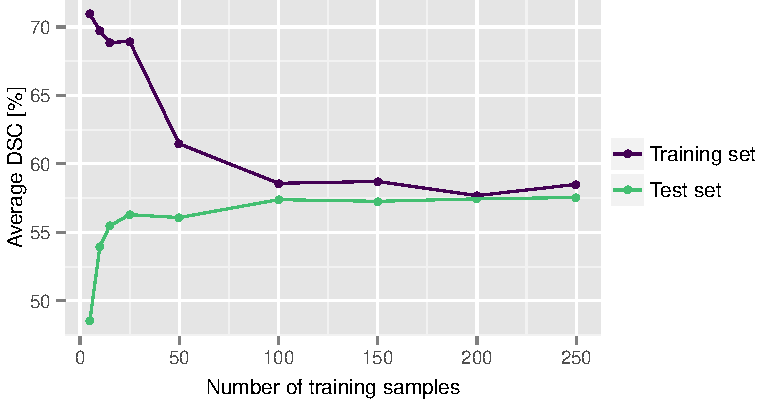
\includegraphics[width=0.8\textwidth]{figures/train_count}
\caption[Comparison of DSC scores calculated on the training and test sets for
varying numbers of training samples]{Comparison of DSC scores calculated on the
training and test sets for varying numbers of training samples. At around 100
samples, the model becomes stable in terms of test performance and the small
difference between training and test DSCs, indicating that overfitting of the
training data no longer occurs.}
\label{fig:bioms}
\end{figure}

\subsection{Comparison on Public Data Sets}

To allow for a direct comparison with a large number of state-of-the-art
methods, we evaluated our method on the MICCAI 2008 MS lesion segmentation
challenge \citep{styner20083d} and the ISBI 2015 longitudinal MS lesion
segmentation challenge. As shown in the previous section, approximately 100
images are required to train the 3-layer CEN without overfitting and we expect
the required number of images to be even higher when adding more layers.
Due to the relatively small size of the training data sets provided by the two
challenges, we used a CEN with only three layers on these data sets to reduce
the risk of overfitting. The parameters of the models are summarized in
\ref{tab:archchallenge}.

\begin{table}[tb]
\caption[Parameters of the 3-layer CEN for the evaluation on the challenge data
sets]{Parameters of the 3-layer CEN for the evaluation on the challenge data
sets. The number of input channels $c$ is 3 for the MICCAI challenge and 4 for
the ISBI challenge.}
\label{tab:archchallenge}
\centering
\begin{tabular}{@{}lccr@{}}
\toprule
Layer type & Kernel Size & \#Filters & \multicolumn{1}{c}{Image Size} \\
\midrule
Input & --- & --- & $164\times 206\times 156\times c$\phantom{0} \\
Convolutional & $9\times 9\times 9\times c$\phantom{0} & 32 &
\num{156x198x148x32} \\
Deconvolutional & \num{9x9x9x32} & 1 & \num{164x206x156x1}\phantom{0} \\
\bottomrule
\end{tabular}
\end{table}

\begin{figure}[tb]
\centering
\small
\def\MRIwidth{0.15\textwidth}

\begin{tikzpicture} 
\tikzstyle{leftlabel}=[rotate=90, align=center,overlay,above]

\matrix [matrix of nodes, nodes={anchor=center, inner sep=1pt}] {
        &[4pt] FLAIR & T1w & T2w & Ground truth & Our method \\[4pt]
\node[leftlabel] {CHB\,07\\(DSC\,=\,\SI{60.58}{\percent})}; &
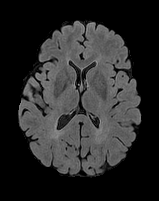
\includegraphics[width=\MRIwidth]{figures/MICCAI2015_CHB07-FLAIR-s88} &
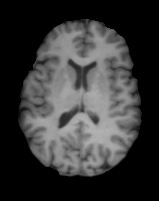
\includegraphics[width=\MRIwidth]{figures/MICCAI2015_CHB07-T1w-s88} &
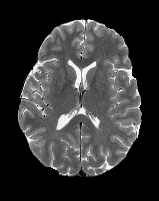
\includegraphics[width=\MRIwidth]{figures/MICCAI2015_CHB07-T2w-s88} &
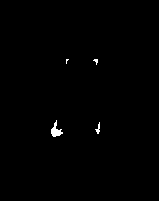
\includegraphics[width=\MRIwidth]{figures/MICCAI2015_CHB07-gold-s88} &
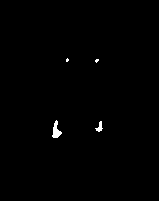
\includegraphics[width=\MRIwidth]{figures/MICCAI2015_CHB07-pred-s88} \\
\node[leftlabel] {CHB\,04\\(DSC\,=\,\SI{61.37}{\percent})}; &
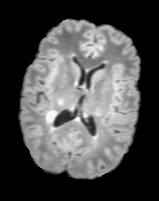
\includegraphics[width=\MRIwidth]{figures/MICCAI2015_CHB04-FLAIR-s85} &
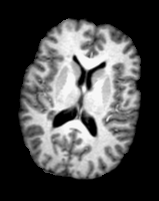
\includegraphics[width=\MRIwidth]{figures/MICCAI2015_CHB04-T1w-s85} &
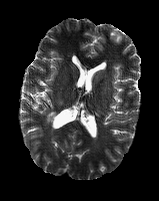
\includegraphics[width=\MRIwidth]{figures/MICCAI2015_CHB04-T2w-s85} &
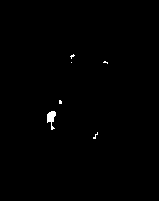
\includegraphics[width=\MRIwidth]{figures/MICCAI2015_CHB04-gold-s85} &

\includegraphics[width=\MRIwidth]{figures/MICCAI2015_CHB04-pred-s85} \\
\node[leftlabel] {UNC\,09\\(DSC\,=\,\SI{9.01}{\percent})}; &
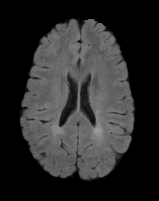
\includegraphics[width=\MRIwidth]{figures/MICCAI2015_UNC09-FLAIR-s89} &
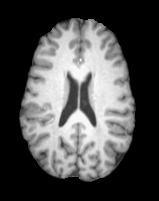
\includegraphics[width=\MRIwidth]{figures/MICCAI2015_UNC09-T1w-s89} &
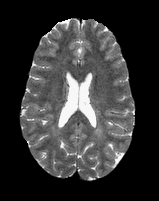
\includegraphics[width=\MRIwidth]{figures/MICCAI2015_UNC09-T2w-s89} &

\includegraphics[width=\MRIwidth]{figures/MICCAI2015_UNC09-gold-s89} &

\includegraphics[width=\MRIwidth]{figures/MICCAI2015_UNC09-pred-s89} \\
};
\end{tikzpicture}

\caption[Example segmentations of our method for three different subjects from
the MICCAI challenge data set]{Example segmentations of our method for three
different subjects from the MICCAI challenge data set. Our method performed well
and consistently despite the large contrast differences seen between the first
two rows. In the third row, our method also segmented lesions that have similar
contrast, but these regions had not been identified as lesions by the manual
rater, which highlights the difficulty in distinguishing focal lesions from
diffuse damage, even for experts.}

\label{fig:segmentation}
\end{figure}

\subsubsection{MICCAI 2008 MS Lesion Segmentation Challenge}

\ref{fig:segmentation} shows a comparison of three subjects from the MICCAI
challenge data set. The first two rows show the FLAIR, T1w, T2w, ground truth
segmentations, and predicted segmentations of two subjects with a DSC of
\SI{60.58}{\percent} and \SI{61.37}{\percent}. Despite the large contrast
differences between the two subjects, our method performed well and
consistently, which indicates that our model was able to learn features that are
robust to a large range of intensity variations. The last row shows a subject
with a DSC of \SI{9.01}{\percent}, one of the lowest DSC scores from the data
set. Our method segmented lesions that have similar contrast to the other two
subjects, but these regions were not classified as lesions by the manual rater.
This highlights the difficulty of manual lesion segmentation, as the difference
between diffuse white matter pathology and focal lesions is often indistinct. A
quantitative comparison of our method with other state-of-the-art methods is
summarized in \ref{tab:state}. Our method outperforms the winning method
\citep{souplet2008} of the MS lesion segmentation challenge 2008 and the
currently best unsupervised method reported on that data set \citep{weiss2013}
in terms of mean TPR and PPV. Our method performs comparably to a current method
\citep{geremia2010} that uses a carefully designed set of features specifically
designed for lesion segmentation, despite our method having learned its features
solely from a relatively small training set.

\begin{table}[tb]
\def\tabspace{12pt}

\caption[Comparison of our method with state-of-the-art lesion segmentation
methods]{Comparison of our method with state-of-the-art lesion segmentation
methods in terms of mean TPR, PPV, and DSC on the training set of the MICCAI
2008 lesion segmentation challenge. Our method performs comparably to the best
methods reported on the MS lesion segmentation challenge data set.}

\label{tab:state}
\centering
\begin{tabular}{l%
@{\hspace{\tabspace}}S[table-format=2.2]
@{\hspace{\tabspace}}S[table-format=2.2]
@{\hspace{\tabspace}}S[table-format=2.2]
}
\toprule
Method & {TPR} & {PPV} & {DSC} \\ 
\midrule
\citet{souplet2008} & 20.65 & 30.00 & {---} \\ 
\citet{weiss2013} & 33.00 & 36.85 & 29.05 \\ 
\citet{geremia2010} & 39.85 & 40.35 & {---}  \\
Our method & 39.71 & 41.38 & 35.52 \\
\bottomrule
\end{tabular}
\end{table}

A comparison of our method with other state-of-the-art methods evaluated on the
MICCAI challenge test data set is summarized in \ref{tab:miccai}. Our method
ranked 6th (2nd if only considering methods with only one submission, i.e.,
without subsequent parameter-tuning and adjustments) out of 52 entries submitted
to the challenge, outperforming the recent SLS by \citet{roura2015}, and popular
methods such as the random forest approach by \citet{geremia2010}, and
Lesion-TOADS by \citet{shiee2010topology}, but not as well as the patch-based
segmentation approach by \citet{guizard2015}, or the MOPS approach by
\citet{tomas2015}, which used additional images to build the intensity model of
a healthy population. This is a very promising result for the first submission
of our method given the simplicity of the model and the small training set size.

\begin{table}[tb]
\sisetup{
  round-mode = places,
  round-precision = 2}%
\caption[Selected methods out of the 52 entries submitted for evaluation to the
MICCAI 2008 MS lesion segmentation challenge]{Selected methods out of the 52
entries submitted for evaluation to the MICCAI 2008 MS lesion segmentation
challenge. Columns LTPR, LFPR, and VD show the average computed from the two
raters in percent. Challenge results last updated: Dec 15, 2015.}
\label{tab:miccai}
\centering
\begin{tabular}{@{}clS[table-format=2.2]
S[table-format=2.1,round-precision=1]
S[table-format=2.1,round-precision=1]
S[table-format=2.1,round-precision=1]@{}}
\toprule
Rank & Method & {Score} & {LTPR} & {LFPR} & {VD} \\
\midrule
$1,3,9$  & \citet{jesson2015} & 86.9386 & 48.70 & 28.25 & 80.15 \\
2  & \citet{guizard2015}   & 86.1071 & 49.85 & 42.75 & 48.80 \\
$4,20,26$  & \citet{tomas2015} & 84.464 & 46.9 & 44.6 &
45.60 \\
$5,7$ & \citet{jerman2015}        & 84.1555 & 65.15 & 63.75 & 77.45 \\
6  & Our method    & 84.0743 & 51.55 & 51.25 & 57.75 \\
11 & \citet{roura2015} & 82.3442 & 50.15 & 41.85 & 111.60 \\
13 & \citet{geremia2010}     & 82.0691 & 55.1 & 74.1 & 48.90 \\
24 & \citet{shiee2010topology} & 79.8975 & 52.4 & 72.7 & 74.45 \\
\bottomrule
\end{tabular}
\end{table}

\subsubsection{ISBI 2015 Longitudinal MS Lesion Segmentation Challenge}

In addition, we evaluated our method on the 21 publicly available labeled cases
from the ISBI 2015 longitudinal MS lesion segmentation challenge. The challenge
organizers have only released the names of the top three teams, only two of
which have published a summary of their mean DSC, LTPR, and LFPR scores for both
raters to allow for a direct comparison. Following the evaluation protocol of
the second \citep{jesson2015} and third \citep{maier2015} place methods, we
trained our model using leave-one-subject-out cross-validation on the training
images and compared our results to the segmentations provided by both raters.
\ref{tab:isbi} summarizes the performance of our method, the two other
methods for comparison, and the performance of the two raters when compared
against each other. Compared to the second and third place methods, our method
was more sensitive and produced significantly higher LTPR scores, but also had
more false positives, which resulted in slightly lower but still comparable DSC
scores. This is again a promising result on a public data set.

\begin{table}[tb]
\caption[Comparison of our method with the second and third ranked methods from
the ISBI MS lesion segmentation challenge]{Comparison of our method with the
second and third ranked methods from the ISBI MS lesion segmentation challenge.
The evaluation was performed on the training set using leave-one-subject-out
cross-validation. GT1 and GT2 denote that the model was trained with the
segmentations provided by the first and second rater as the ground truth,
respectively.}
\label{tab:isbi}
\centering
\begin{tabular}{@{}lcccccc@{}}
\toprule
Method &
\multicolumn{3}{c}{Rater 1} &
\multicolumn{3}{c}{Rater 2} \\
& DSC & LTPR & LFPR & DSC & LTPR & LFPR \\
\midrule
Rater 1 & --- & --- & --- & 73.2 & 64.5 & 17.4 \\
Rater 2 & 73.2 & 82.6 & 35.5 & --- & --- & --- \\
\citet{jesson2015} &  70.4 & 61.1 & 13.5 & 68.1 & 50.1 & 12.7 \\
\citet{maier2015} (GT1) & 70 & 53 & 48 & 65 & 37 & 44 \\
\citet{maier2015} (GT2) & 70 & 55 & 48 & 65 & 38 & 43 \\
Our method (GT1) & 68.4 & 74.5 & 54.5 & 64.4 & 63.0 & 52.8 \\
Our method (GT2) & 68.3 & 78.3 & 64.5 & 65.8 & 69.3 & 61.9 \\
\bottomrule
\end{tabular}
\end{table}

\subsection{Comparison of Network Architectures, Input Modalities, and
Publicly Available Methods on Clinical Trial Data}

\begin{table}[tb]
\caption{Parameters of the 3-layer CEN used on the clinical trial data set.}
\label{tab:arch3}
\centering
\begin{tabular}{@{}lccr@{}}
\toprule
Layer type & Kernel Size & \#Filters & \multicolumn{1}{c}{Image Size} \\
\midrule
Input & --- & --- & \num{164x206x52x2}\phantom{0} \\
Convolutional & \num{9x9x5x2} & 32 & \num{156x198x48x32} \\
Deconvolutional & \num{9x9x5x32} & 1 & \num{164x206x52x1}\phantom{0} \\
\bottomrule
\end{tabular}
\end{table}

\subsubsection{Quantitative Comparison}

To determine the effect of network architectures, we compared the segmentation
performance of three different networks using T1w and FLAIR MRIs.
Specifically, we trained a 3-layer CEN and two 7-layer CENs, one with shortcut
connections and one without. To investigate the effect of different input image
types, we additionally trained two 7-layer CEN-s on the modalities used by EMS
(T1w, T2w, PDw) and all four modalities (T1w, T2w, PDw, FLAIR). The parameters
of the networks are given in \ref{tab:arch3} and \ref{tab:arch7}. To
roughly compensate for the anisotropic voxel size of the input images, we chose
an anisotropic filter size of \num{9x9x5}. In addition, we ran the five
competing methods discussed in \ref{sec:othermethods} with Lesion-TOADS, SLS,
and the two LST methods using the T1w and FLAIR images, and EMS using three
(T1w, T2w, PDw) and all four modalities in separate tests. A comparison of the
segmentation accuracy of the trained networks and competing methods is
summarized in \ref{tab:results1}.

\begin{table}[tb]
\caption{Parameters of the 7-layer CEN-s used on the clinical trial data set.}
\label{tab:arch7}
\centering
\begin{tabular}{@{}lccr@{}}
\toprule
Layer type & Kernel Size & \#Filters & \multicolumn{1}{c}{Image Size} \\
\midrule
Input & --- & --- & \num{164x206x52x2}\phantom{0} \\
Convolutional & \num{9x9x5x2} & 32 & \num{156x198x48x32} \\
{Average Pooling} & \num{2x2x2} & --- & \num{78x99x24x32} \\
{Convolutional} & \num{9x10x5x32} & 32 & \num{70x90x20x32} \\
{Deconvolutional} & \num{9x10x5x32} & 32 & \num{78x99x24x32} \\
{Unpooling }& \num{2x2x2} & --- & \num{156x198x48x32} \\
{Deconvolutional }& \num{9x9x5x32} & 1 & \num{164x206x52x1}\phantom{0} \\
\bottomrule
\end{tabular}
\end{table}

\begin{table}[tb]
\caption[Comparison of the segmentation accuracy of different CEN models, other
methods, and input modalities.]{Comparison of the segmentation accuracy of
different CEN models, other methods, and input modalities. The table shows the
mean of the Dice similarity coefficient (DSC), lesion true positive rate (LTPR),
and lesion false positive rate (LFPR). Because the volume difference (VD) is not
limited to the interval $[0, 100]$, a single outlier can heavily affect the
calculation of the mean. We therefore excluded outliers before calculating the
mean of the VD for all methods using the box plot criterion.}
\centering
\small
\label{tab:results1}
\begin{tabular}{@{}lcccc@{}}
\toprule
Method & DSC [\%] & LTPR [\%] & LFPR [\%] & VD [\%] \\
\midrule
\multicolumn{5}{c}{\textit{Input modalities: T1w and FLAIR}} \\
\midrule
3-layer CEN & 49.24 & 57.33 & 61.39 & 43.45 \\
7-layer CEN & 52.07 & 43.88 & 29.06 & 37.01 \\ 
7-layer CEN-s & 55.76 & 54.55 & 38.64 & 36.30 \\[0.2em]
Lesion-TOADS \citep{shiee2010topology} & 40.04 & 56.56 & 82.90 & 49.36 \\ 
SLS \citep{roura2015}  & 43.20 &  56.80 & 50.80 & 12.30 \\
LST-LGA \citep{schmidt2012automated} & 46.64 & 37.50 & 38.06 & 36.77 \\
LST-LPA \citep{schmidt2012automated} & 46.07 & 48.02 & 52.94 & 41.62 \\
\midrule
\multicolumn{5}{c}{\textit{Input modalities: T1w, T2w, and PDw}} \\
\midrule
7-layer CEN-s & 61.18 & 52.00 & 36.68 & 29.38 \\
EMS \citep{vanleemput2001} & 42.94 & 44.80 & 76.58 & 49.29 \\
\midrule
\multicolumn{5}{c}{\textit{Input modalities: T1w, T2w, FLAIR, and PDw}} \\
\midrule
7-layer CEN-s & 63.83 & 62.49 & 36.10 & 32.89 \\
EMS \citep{vanleemput2001} & 39.70 & 49.08 & 85.01 & 34.51 \\
\bottomrule
\end{tabular}
\end{table}

All CEN architectures performed significantly better than all other methods
regardless of the input modalities, with LST-LGA being the closest in overall
segmentation accuracy. Comparing CEN to LST-LGA, the improvements in the mean
DSC scores ranged from 3 percentage points (pp) for the 3-layer CEN to 17\,pp
for the 7-layer CEN with shortcut trained on all four modalities. The improved
segmentation performance was mostly due to an increase in lesion sensitivity.
LST-LGA achieved a mean lesion TPR of \SI{37.50}{\percent}, compared to
\SI{54.55}{\percent} produced by the CEN with shortcut when trained on the same
modalities, and \SI{62.49}{\percent} when trained on all four modalities, while
achieving a comparable number of lesion false positives. The mean lesion FPRs
and mean volume differences of LST-LGA and the 7-layer CEN-s were very close,
when trained on the same modalities, and the CEN-s further reduced its FPR when
trained on more modalities.

This experiment also showed that increasing the depth of the CEN and adding the
shortcut connections both improve the segmentation accuracy. Increasing the
depth of the CEN from three layers to seven layers improved the mean DSC by
3\,pp. The improvement was confirmed to be statistically significant using a
one-sided paired $t$-test ($p$-value of \num{1.3e-5}). Adding a shortcut to the
network further improved the segmentation accuracy as measured by the DSC by
3\,pp. A second one-sided paired $t$-test was performed to confirm the
statistical significance of the improvement with a $p$-value of less than
\num{1e-10}.

\subsubsection{Qualitative Comparison of Network Architectures}

The impact of increasing the depth of the network on the segmentation
performance of very large lesions is illustrated in \ref{fig:large}, where the
true positive, false negative, and false positive voxels are highlighted in
green, yellow, and red, respectively. The receptive field of the 3-layer CEN has
a size of only \num{17x17x9} voxels, which reduces its ability to identify very
large lesions marked by two white circles. In contrast, the 7-layer CEN has a
receptive field size of \num{49x53x26} voxels, which allows it to learn features
that can capture much larger lesions. Consequently, the 7-layer CEN, with and
without shortcut, is able to learn a feature set that captures large lesions
much better than the 3-layer CEN, which results in an improved segmentation.
However, increasing the depth of the network

\begin{figure}[p]
\centering
\begin{tikzpicture}[node distance=3.2cm and 0.3\textwidth,
  font=\small, on grid]
\node[inner sep=0] (image1) {
  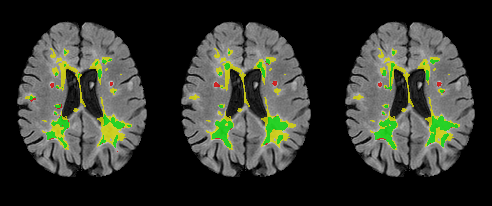
\includegraphics[width=0.9\textwidth]{figures/tmi/p50s35_large_lesions}
};
\node[above=of image1] (l7) {7-layer CEN};
\node[left=of l7] {3-layer CEN};
\node[right=of l7] {7-layer CEN-s};

\begin{scope}[xshift=0.3\textwidth,scale=1.6]
\draw[white,thick] (-12pt,-15pt) circle (9pt);
\draw[white,thick] (15pt,-15pt) circle (10pt);
\end{scope}
\begin{scope}[xshift=-0.3\textwidth,scale=1.6]
\draw[white,thick] (-12pt,-15pt) circle (9pt);
\draw[white,thick] (15pt,-15pt) circle (10pt);
\end{scope}
\begin{scope}[scale=1.6]
\draw[white,thick] (-12pt,-15pt) circle (9pt);
\draw[white,thick] (15pt,-15pt) circle (10pt);
\end{scope}
\end{tikzpicture}
\caption[Impact of increasing the depth of the network on the segmentation
performance of very large lesions]{Impact of increasing the depth of the network on the segmentation
performance of very large lesions. The true positive, false negative, and false
positive voxels are highlighted in green, yellow, and red, respectively. The
7-layer CEN, with and without shortcut, is able to segment large lesions much
better than the 3-layer CEN due to the increased size of the receptive field.
This figure is best viewed in color.}
\label{fig:large}
\end{figure}

\begin{figure}[p]
\centering
\begin{tikzpicture}[node distance=3.2cm and 0.3\textwidth,
  font=\small, on grid,spy using outlines={circle, connect spies}]
  
\node[inner sep=0] (image1) {
  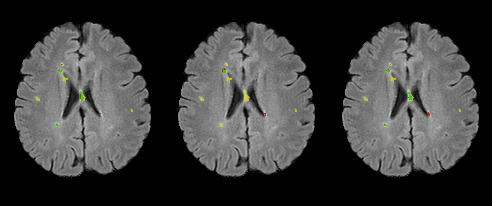
\includegraphics[width=0.9\textwidth]{figures/tmi/p25s35_small_lesions}
};
\node[above=of image1] (l7) {7-layer CEN};
\node[left=of l7] {3-layer CEN};
\node[right=of l7] {7-layer CEN-s};

\begin{scope}[xshift=0.3\textwidth]
\coordinate (on1) at (-15.2pt,30.5pt);
\coordinate (in1) at (-32pt,54pt);
\spy[white,thick,size=40pt,magnification=6] on (on1) in node[overlay] at (in1);

\coordinate (on2) at (0pt,5.5pt);
\coordinate (in2) at (28pt, 50pt);
\spy[white,thick, size=54pt, magnification=3.5, xshift=0.3\textwidth] on
(on2) in node[overlay] at (in2);

\coordinate (on3) at (-19.5pt,-18pt);
\coordinate (in3) at (10pt,-52pt);
\spy[white,thick, size=40pt, magnification=6, xshift=0.3\textwidth] on
(on3) in node[overlay] at (in3);
\end{scope}

\begin{scope}[xshift=-0.3\textwidth]
\coordinate (on4) at (-15.2pt,30.5pt);
\coordinate (in4) at (-32pt,54pt);
\spy[white,thick,size=40pt,magnification=6] on (on4) in node[overlay] at (in4);

\coordinate (on5) at (0pt,5.5pt);
\coordinate (in5) at (28pt, 50pt);
\spy[white,thick, size=54pt, magnification=3.5, xshift=0.3\textwidth] on
(on5) in node[overlay] at (in5);

\coordinate (on6) at (-19.5pt,-18pt);
\coordinate (in6) at (10pt,-52pt);
\spy[white,thick, size=40pt, magnification=6, xshift=0.3\textwidth] on
(on6) in node[overlay] at (in6);
\end{scope}

\spy[white,thick, size=40pt, magnification=6] on (-15.2pt,30.5pt)
in node[overlay] at (-32pt,54pt);
\spy[white,thick, size=54pt, magnification=3.5] on (0pt,5.5pt)
in node[overlay] at (28pt, 50pt);
\spy[white,thick, size=40pt, magnification=6] on (-19.5pt,-18pt)
in node[overlay] at (10pt,-52pt);
\end{tikzpicture}

\caption[Comparison of segmentation performance of different CEN architectures
for small lesions]{Comparison of segmentation performance of different CEN architectures
for small lesions. The white circles indicate lesions that were detected by the
3-layer CEN and the 7-layer CEN, but only with shortcut. Increasing the network
depth decreases the sensitivity to small lesions, but the addition of a
shortcut allows the network to regain this ability, while still being able to
detect large lesions (see \ref{fig:large}). This figure is best viewed in
color.}
\label{fig:small}
\end{figure}

% TODO: check that the page break hasn't changed 

\noindent without adding shortcut connections
reduces the network's sensitivity to very small lesions as illustrated in
\ref{fig:small}. In this example, the 3-layer CEN was able to detect three small
lesions, indicated by the white circles, which were missed by the 7-layer CEN.
Adding shortcut connections enables our model to learn a feature set that spans
a wider range of lesion sizes, which increases the sensitivity to small lesions
and, hence, allows the 7-layer \mbox{CEN-s} to detect all three small lesions
(highlighted by the white circles), while still being able to segment large
lesions.

\subsection{Comparison for Different Lesion Sizes}

\begin{table}[tb]
\caption{Lesion size groups as used for the detailed analysis.}
\label{tab:groups}
\centering
\begin{tabular}{@{}lccc@{}}
\toprule
Group & Mean lesion size [\si{\cubic\milli\metre}] & \#Samples & Lesion
load [\si{\cubic\milli\metre}] \\
\midrule
Very small & $[0,70]$ & 6 & \num{1457+-1492} \\
Small      & $(70,140]$ & 24 & \num{4298+-2683} \\
Medium & $(140,280]$ & 24 & \num{12620+-9991} \\
Large & $(280,500]$ & 14 & \num{13872+-5814} \\
Very large & $> 500$ & 9 & \num{35238+-27531} \\
\bottomrule
\end{tabular}
\end{table}

\begin{figure}
\centering
%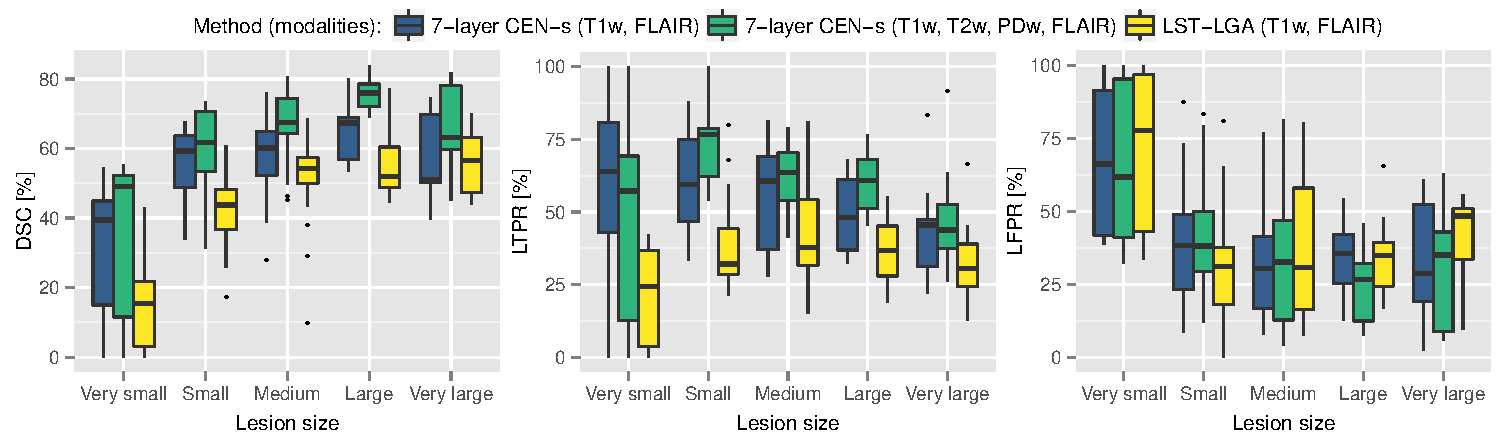
\includegraphics[width=\textwidth]{figures/tmi/cen_vs_LGA_size}
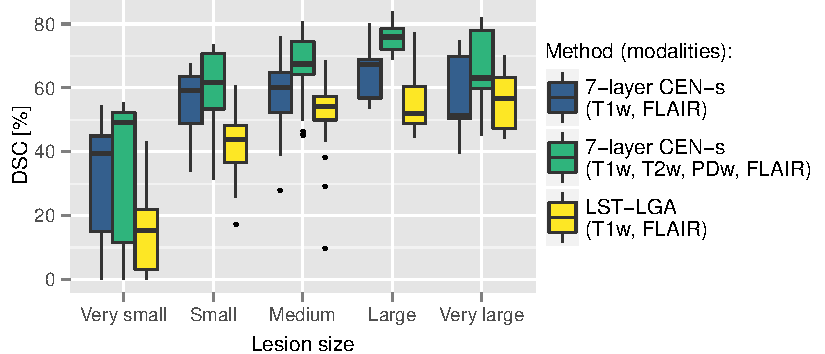
\includegraphics[width=0.78\textwidth]{figures/tmi/dsc}
\\[1em]
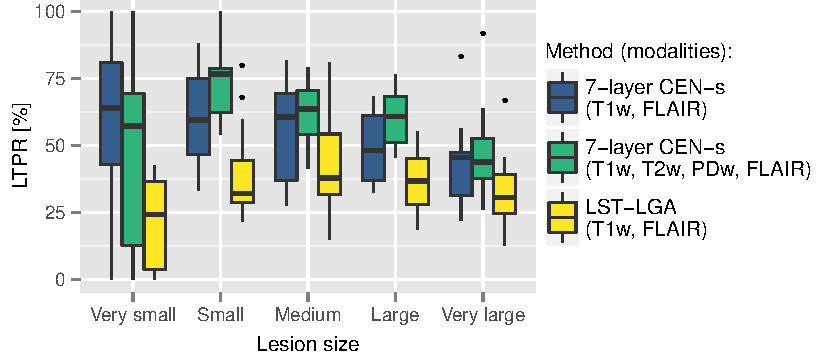
\includegraphics[width=0.78\textwidth]{figures/tmi/tpr}
\\[1em]
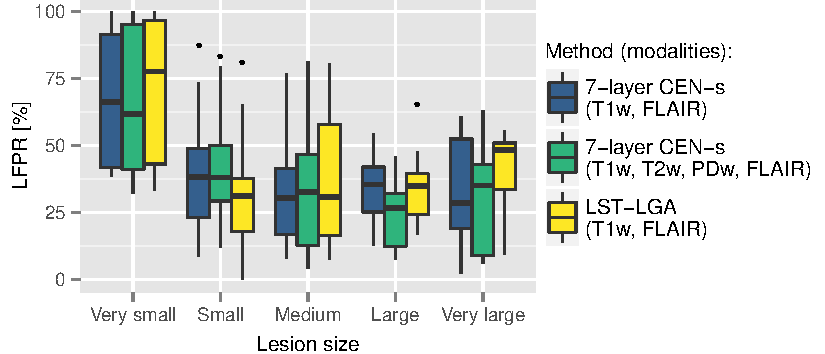
\includegraphics[width=0.78\textwidth]{figures/tmi/fpr}

\caption[Comparison of segmentation accuracy and lesion detection measures of a
7-layer CEN-s trained on different input modalities and the best performing
competing method LST-LGA for different lesion sizes]{Comparison of segmentation accuracy and lesion detection measures of
a 7-layer CEN-s trained on different input modalities and the best performing
competing method LST-LGA for different lesion sizes. The 7-layer CEN-s
outperforms LST-LGA for all lesions sizes except for very large lesions when
trained on T1w and FLAIR MRIs, and for all lesion sizes when trained on all four
modalities, due to a higher sensitivity to lesions, while producing
approximately the same number of false positives. Outliers are denoted by black
dots.}

\label{fig:sizecomp}
\end{figure}

To examine the effect of lesion size on segmentation performance, we stratified
the test set into five groups based on their mean reference lesion size as
summarized in \ref{tab:groups}. A comparison of segmentation accuracy and lesion
detection measures of a 7-layer CEN-s trained on different input modalities and
the best performing competing method LST-LGA for different lesion sizes is
illustrated in \ref{fig:sizecomp}. The 7-layer CEN-s outperformed LST-LGA for
all lesions sizes except for very large lesions when trained on T1w and FLAIR
MRIs. The advantage extended to all lesion sizes when the \mbox{CEN-s} was
trained on all four modalities, which could not be done for LST-LGA.
The differences were larger for smaller lesions, which are generally more
challenging to segment for all methods. The differences between the two
approaches were due to a higher sensitivity to lesions as measured by the LTPR,
especially for smaller lesions, while the number of false positives was
approximately the same for all lesion sizes.

\section{Discussion}

The automatic segmentation of MS lesions is a very challenging task due to the
large variability in lesion size, shape, intensity, and location, as well as the
large variability of imaging contrasts produced by different scanners used in
multi-center studies. Most unsupervised methods model lesions as an outlier
class or a separate cluster in a subject-specific model, which makes them
inherently robust to inter-subject and inter-scanner variability. However,
outliers are often not specific to lesions and can also be caused by intensity
inhomogeneities, partial volume, imaging artifacts, and small anatomical
structures such as blood vessels, which leads to the generation of false
positives. On the other hand, supervised methods can learn to discriminate
between lesion and non-lesion tissue, but are more sensitive to the variability
in lesion appearance and different contrasts produced by different scanners. To
overcome those challenges, supervised methods require large data sets that span
the variability in lesion appearance and careful pre-processing to match the
imaging contrast of new images with those of the training set. Library-based
approaches have shown great promise for the segmentation of MS lesions, but do
not scale well to very large data sets due to the large amount of memory
required to store comprehensive sample libraries and the time required to scan
such libraries for matching patches. On the other hand, parametric deep learning
models such as convolutional neural networks scale much better to large training
sets, because the size required to store the model is independent of the
training set size, and the operations required for training and inference are
inherently parallelizable, which allows them to take advantage of very fast
GPU-accelerated computing hardware. Furthermore, the combination of many
nonlinear processing units allows them to learn features that are robust under
large variability, which is crucial for the segmentation of MS lesions.

Convolutional neural networks were originally designed to classify entire images
and designing networks that can segment images remains an important research
topic. Early approaches have formulated the segmentation problem as a patch-wise
classification problem, which allows them to directly use established
classification network architectures for image segmentation.
However, a major limitation of patch-based deep learning approaches is the time
required for training and inference. Fully convolutional networks can perform
the segmentation much more efficiently, but generally lack the precision to
perform voxel-accurate segmentation and cannot handle unbalanced classes.

To overcome these challenges, we have presented a new method for the automatic
segmentation of MS lesions based on deep convolutional encoder networks with
shortcut connections. The joint training of the feature extraction and
prediction pathways allows for the automatic learning of features at different
scales that are tuned for a given combination of image types and segmentation
task. Shortcuts between the two pathways allow high- and low-level features to
be leveraged at the same time for more consistent performance across scales. In
addition, we have proposed a new objective function based on the combination of
sensitivity and specificity, which makes the objective function inherently
robust to unbalanced classes such as MS lesions, which typically comprise less
than \SI{1}{\percent} of all image voxels. We have evaluated our method on two
publicly available data sets and a large data set from an MS clinical trial,
with the results showing that our method performs comparably to the best
state-of-the-art methods, even for relatively small training set sizes. We have
also shown that when a suitably large training set is available, our method is
able to segment MS more accurately than widely-used competing methods such as
EMS, LST-LGA, SLS, and Lesion-TOADS. The substantial gains in accuracy were
mostly due to an increase in lesion sensitivity, especially for small lesions.
Overall, our proposed CEN with shortcut connections performed consistently well
over a wide range of lesion sizes.

Our segmentation framework is very flexible and can be easily extended. One such
extension could be to incorporate prior knowledge about the tissue type of each
non-lesion voxel into the segmentation procedure. The probabilities of each
tissue class could be precomputed by a standard segmentation method, after which
they can be added as an additional channel to the input units of the CEN, which
would allow the CEN to take advantage of intensity information from different
modalities and prior knowledge about each tissue class to carry out the
segmentation. In addition, our method can be applied to other segmentation
tasks. Although we have only focused on the segmentation of MS lesions in this
paper, our method does not make any assumptions specific to MS lesion
segmentation. The features required to carry out the segmentation are solely
learned from training data, which allows our method to be used to segment
different types of pathology or anatomy when a suitable training set is
available.

\chapter{Manifold Learning by Deep Learning}
\label{sec:manifold}

\section{Introduction}

% Start with section on manifold learning of AD and MS
% populations. Including a summary of those methods and the whole literature
% review of what has been done. This includes manifold learning, population
% studies, disease classification and the likes without deep learning.

\begin{comment}

What is manifold learning?

Why are we doing it?


\end{comment}

% In this chapter, we will use manifold learning to detect patterns of variability
% in groups of images. Variability is captured in terms of the coordinates in
% manifold space, which can be used as imaging biomarkers for assessing the
% disease state or for classification into different subtypes. In this chapter, we
% propose using a deep learning model called a deep belief network for learning
% the manifold of medical images. The potential of deep learning for manifold
% learning was evaluated on images of AD patients and MS patients.

Changes in brain morphology such as global and regional atrophy and the
formation of white matter lesions are two hallmarks of \gls{ms} pathology. In
order to quantify the pathological manifestation of MS, a number of imaging
biomarkers derived from \gls{mri} scans of the brain, such as lesion volume and
whole brain volume, have been proposed, which have established their importance
for the study of MS. However, MS is a complex disease whose pathological
variability extends well beyond what can be captured by global and local
volumetric measures. It would be highly desirable to have a method that can
automatically discover potentially important patterns of variability in brain
morphology and lesion distribution, which would advance our understanding of the
complex pathology of MS. In addition, the joint modelling of brain morphology and
lesion distribution would further our knowledge of how these two key
pathological features interact. However, this type of modelling is very
challenging due to the high dimensionality of the data.

In recent years, there has been an increased interest in biomarker discovery
using manifold learning to form high-level, low-dimensional representations of
medical images \citep{wolz2010b,aljabar2011,wolz2012}. In order to discover
common patterns of variability in a group of images, each image of the data set
is regarded as a point in a high-dimensional image space (called the ambient
space), with $n_x \times n_y \times n_z$ coordinates, where $n_x, n_y, n_z$ are
the dimensions of each image. On the other hand, each image could also be
identified by a smaller set of parameters that describe shape variations and
patterns that are common for a particular group of images. These parameters span
a new space called the manifold space. The task of manifold learning is to
discover the low-dimensional space and its parameters, which can then be used to
model the anatomical variability within a population, or serve as biomarkers to
track disease state and progression.

In the remainder of this section, we will briefly revise common manifold
learning techniques and applications for medical image analysis. A main part of
the chapter will be an explanation of the deep learning manifold learning
framework using a deep belief network. We have evaluated the proposed manifold
learning method on two tasks: a) to learn the variability of \gls{mr} images of
the brain of \gls{ad} patients, and b) to discover patterns of morphological
variability and lesion distribution in MS.

\section[Manifold learning for medical image analysis]{Manifold Learning for
Medical Image Analysis}

Most popular manifold learning methods for medical image analysis can be roughly
classified into local and global methods \citep{cayton2005}. Local algorithms
such as \gls{lle} \citep{saul2003} and \gls{lem} \citep{belkin2002} try to find a low
dimensional representation of the data such that local distances between points
in ambient space are best preserved when mapped to manifold space. In contrast,
global methods such as \gls{isomap} \citep{tenenbaum2000} try to find an
embedding of the manifold space that best preserves geodesic distances of points
that lie far apart in ambient space. Both types of methods require building a
proximity graph that is used to capture neighborhood information (local methods)
or to estimate geodesic distances by calculating the shortest path distances
between all points on the affinity graph (global methods). Both types of methods
assume that the manifold is locally linear, which means that distances between
neighboring points in manifold space can be approximated by their distances in
ambient space. Once the proximity graph has been created, a unique solution to
the inherent optimization problem of each algorithm can be found analytically by
solving an eigenvalue problem.

\begin{comment}

Applications:
- regularize segmentation of the heart ventricles
- regularize segmentation of the brain ventricles
- constrain registration
- clinical predictions
- biomarker discovery
- atlas propagation for the segmentation of the hippocampus
- discriminate between normal and abnormal motion patterns of the heart
- feature extraction
- similarity measure for images -> prediction of AD
- classification of Alzheimer's disease
- extract features representing inter-subject variability

\end{comment}

Manifold learning methods have been successfully applied to various image
analysis problems such as the segmentation of the hippocampus \citep{wolz2010},
to regularize the segmentation of heart \citep{zhang2006} and brain
ventricles~\citep{etyngier2007}, and to constrain the deformable registration of
brain images to have biologically plausible parameters \citep{hamm2010}, while
most methods focus on clinical prediction
\citep{gerber2010,wolz2012,duchateau2012,aljabar2011,wachinger2015,bhatia2012,
guerrero2014}. Gerber et al. used Isomap to predict clinical parameters of AD
patients \citep{gerber2009,gerber2010}, and Wolz et al. used LEM to perform
biomarker discovery \citep{wolz2011,wolz2012}, also of AD patients.
\citet{duchateau2011,duchateau2012} discriminate between normal and abnormal
motion patterns of the heart based on the definition of pathology as a deviation
from normality. After learning the manifold representing normal motion
patterns, abnormal motion patterns can be detected based on the
distance of a new data sample from the manifold surface.
% \citet{aljabar2010,aljabar2011} proposed a method for the joint modelling of
% multiple image features of neonatal brains. First, separate manifolds based on
% features from geometric surface models, non-rigid deformations, and image
% intensities are learned, then a second dimensionality reduction step is used
% to combine the individual manifold parameters.
\citet{wachinger2015} proposed a new shape descriptor of the brain called
BrainPrint, which is build by solving the eigenvalue problem of the 2D and 3D
Laplace-Beltrami operator on meshes of segmented cortical and subcortical
structures. The descriptor defines a similarity measure on brain images, which
can be used to perform subject identification \citep{wachinger2014a}, and to
predict Alzheimer's disease \citep{wachinger2014b}.
\citet{bhatia2012} model regional variations of the brain by building a manifold
on hierarchical image patches and applied it to finding discriminative regions
of 3D brain \gls{mr} images for classifying Alzheimer's disease.
\citet{guerrero2014} have used manifold learning on \glspl{roi} to
extract features that represent inter-subject variability of AD patients.
In a first step, sparse regression is used to automatically detect the
\gls{roi} using \gls{mmse} scores as the independent
variable. Then, LEM with cross-correlation as the distance measure is used to
learn the manifold of the ROIs, from which the features are extracted.

A main challenge of most manifold learning methods (e.g., Isomap, LEM, LLE) is
the construction of the proximity graph. Building the proximity graph requires
choosing an appropriate neighborhood criterion, which can be challenging due to
the sensitivity to noise of commonly used criteria (e.g., $k$-nearest neighbors,
$\epsilon$-ball), and, consequently, may result in an unstable topology of the
learned manifold \citep{balasubramanian2002}. Other challenges include avoiding
erroneously disconnected regions and shortcuts, finding a trade-off between
sampling density and curvature of local patches of the manifold, and finding a
suitable distance metric. A number of solutions have been proposed, but there is
no general solution. To increase the robustness to noise and varying parameter
settings, \citet{carreira2005} proposed building the graph from a graph ensemble
that combines multiple spanning trees, each fit to a perturbed version of the
data set. A trade-off between sampling density and curvature of local patches of
the manifold can be found automatically by adapting the selection of the
neighborhood sizes through neighborhood contraction and expansion
\citep{zhang2012}. \citet{gerber2010} have shown that the choice of a suitable
distance measure is crucial for manifold learning using Isomap and that the
warping distance between brain images improves the learning performance over
previously used Euclidean distances in the image space.

\section[Manifold learning using deep belief networks]{Manifold Learning using
Deep Belief Networks}

Deep generative models such as \glspl{dbn} are a promising alternative to
previously used brain manifold learning methods due to their ability to discover
patterns of similarity in groups of images. In contrast to most commonly used
manifold learning algorithms (e.g., LLE, LEM, Isomap), DBNs do not assume the
manifold space to be locally linear and do not require a previously defined
similarity measure or the construction of a proximity graph, which makes them
more generally applicable to a wide range of manifold learning tasks. This is
particularly important for the application to brain manifold learning, because
the high-dimensionality of brain MRIs make defining a neighborhood criterion
challenging.

% DBNs have been used for many
% different tasks where the choice of an appropriate architecture is crucial for
% the success. In this section, we will explain the choices we made in designing
% the overall manifold learning framework. Particular parameter choices are
% explained along with two applications.

\subsection[General architecture]{General Architecture}
\label{sec:general_arch}

The general architecture of the DBN used for manifold learning of brain MRIs is
illustrated in \ref{fig:manidbn}. The first \gls{rbm} receives the intensity
values of a group of images in ambient space as input and reduces the
dimensionality of each image by discovering patterns of similarity that are
common within groups of images. Subsequent RBMs receive the hidden unit
activations of the previous RBM as input, thus learning successively more
complex and abstract patterns from a training set, where the hidden units of the
last layer represent the coordinates of an image in manifold space. The number
of trainable weights increases significantly with the resolution of the training
images. In order to scale the model to high-resolution images, the first several
layers of our DBN are \glspl{scrbm}, a type of RBM that uses weight sharing and
local connectivity between units of adjacent layers to reduce the number of
trainable weights. Due to the much smaller number of trainable parameters
compared to dense RBMs, sconvRBMs are best suited for learning low- to mid-level
features from very high-dimensional data such as brain MRIs. Compared to other
more commonly used convolution-based RBMs \citep{lee2009}, an advantage of
sconvRBMs is that inference is invertible, which allows the reconstruction of
the visible units from the hidden unit activations. In our application, this
allows for the mapping of parameters from the manifold space back to the ambient
space. Due to the local connectivity of the weights, sconvRBMs can only learn
local patterns in the data. In order to learn patterns that describe images as a
whole, sconvRBM layers are followed by dense RBMs, which integrate the extracted
feature from all image locations in order to model global patterns.

\begin{figure}
\centering
\begin{tikzpicture}[scale=0.85]
\tikzstyle{every node}=[font=\sffamily\small, inner sep=3pt, align=center]
\tikzstyle{every pin}=[align=center,fill=white,overlay]
\tikzstyle{dbnlabel}=[font=\sffamily]
         
% Deformation field
        
%\node[dbnlabel, rotate=90] at (-1.5,2.25) {Morphology DBN};
        
\begin{scope}[xshift=-10pt,yslant=0.63,xscale=0.4]

\node[transform shape,pin={[pin
distance=8]125:Input image}] (field) at (2,2)
{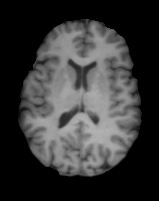
\includegraphics[width=3.45cm]{figures/MICCAI2015_CHB07-T1w-s88}};

% \node[pin={[pin distance=0.6,overlay]93:Displacement\\
% field $u$}] at ($(field.north west)!0.1!(field.north east)$) {};

\end{scope}
         
% 3-channel input

\foreach \x in {20} {
\begin{scope}[xshift=\x pt]
%\ifnum\x=0
%\path
%\else
\draw[fill=white, fill opacity=0.75]
%\fi
  (0,0) coordinate(A\x) -- ++(90:4) coordinate (B\x) -- ++(30:2) coordinate
  (C\x) -- ++(-90:4) -- cycle;
  

% \begin{scope}[xshift=-50pt,yslant=0.63,xscale=0.4]  
% \node[transform shape,inner sep=0pt] at (2,2)
%   {\includegraphics[width=4cm]{deformation2.png}};
% \end{scope}
  
\draw (0,3)
   ++(30:0.25) \ifnum\x=20 coordinate (a1) \else -- +(0:10pt) +(0:0) \fi
-- ++(90:0.5)  \ifnum\x=20 coordinate (b1) \else -- +(0:10pt) +(0:0) \fi
-- ++(30:0.25) \ifnum\x=20 coordinate (c1) \else -- +(0:10pt) +(0:0) \fi
-- ++(-90:0.5) \ifnum\x=20 coordinate (d1) \else -- +(0:10pt) +(0:0) \fi
-- ++(210:0.25);
\end{scope}
}

%\node[below=4pt,xshift=-3pt] at (A0)  {$u_x$};
%\node[below=4pt] at (A10) {$u_y$};
%\node[below=4pt,xshift=3pt] at (A20) {$u_z$};

%\node[pin={[pin distance=5pt]260:$u_x$}] at (A0)  {};
%\node[pin={[pin distance=5pt]270:$u_y$}] at (A10)  {};
%\node[pin={[pin distance=5pt]290:$u_z$}] at (A20)  {};

\draw[decorate,decoration={brace,raise=4pt,mirror}]
(A20) --node[below=8pt] {Visible units} (A20-|C20);

% Transition

\draw ($(a1)!0.5!(c1)$) ++(55pt,-5pt) coordinate (e1);
\draw (a1) -- (e1);
\draw (b1) -- (e1);
\draw (c1) --node[pin={[pin distance=1cm]40:Strided\\ convolution}] {} (e1);
\draw (d1) -- (e1);

% First layer hidden units

\foreach \x in {80,85,90,95,100,105} {
\begin{scope}[xshift=\x pt,yshift=1.5cm,scale=0.5]
\draw[fill=white, fill opacity=0.75]
  (0,0) coordinate(A\x) -- ++(90:4) coordinate (B\x) -- ++(30:2) coordinate
  (C\x) -- ++(-90:4) coordinate(D\x) -- cycle;
   
\draw (0,2.5)
   ++(30:0.25) \ifnum\x=105 coordinate (a2) \else -- +(0:10pt) +(0:0) \fi
-- ++(90:1)    \ifnum\x=105 coordinate (b2) \else -- +(0:10pt) +(0:0) \fi
-- ++(30:0.5)  \ifnum\x=105 coordinate (c2) \else -- +(0:10pt) +(0:0) \fi
-- ++(-90:1)   \ifnum\x=105 coordinate (d2) \else -- +(0:10pt) +(0:0) \fi
-- ++(210:0.5);
\end{scope}
}

\draw[decorate,decoration={brace,raise=20pt}] (B20|-C20) --node[above=25pt]
{Strided convolutional RBM} (C105|-C20);

%\draw[decorate,decoration={brace,raise=4pt,mirror}]
%(A80) --node[below=8pt] {$N = 32$} (A80-|D105);
%(A80) --node[below=8pt] {Hidden units} (A80-|D105);

\draw ($(a2)!0.5!(c2)$) ++(0:38pt) coordinate (e2);
\draw (a2) -- (e2);
\draw (b2) -- (e2);
\draw (c2) -- (e2);
\draw (d2) -- (e2);

% Second layer hidden units

\foreach \x in {145, 150, ..., 175, 180} {
\begin{scope}[xshift=\x pt,yshift=2.25cm,scale=0.25]
\draw[fill=white, fill opacity=0.75]
  (0,0) coordinate(A\x) -- ++(90:4) coordinate (B\x) -- ++(30:2) coordinate
  (C\x) -- ++(-90:4) coordinate(D\x) -- cycle;
\draw (0,1.75)
   ++(30:0.25) \ifnum\x=180 coordinate (a3) \else -- +(0:20pt) +(0:0) \fi
-- ++(90:2)    \ifnum\x=180 coordinate (b3) \else -- +(0:20pt) +(0:0) \fi
-- ++(30:1)    \ifnum\x=180 coordinate (c3) \else -- +(0:20pt) +(0:0) \fi
-- ++(-90:2)   \ifnum\x=180 coordinate (d3) \else -- +(0:20pt) +(0:0) \fi
-- ++(210:1);
\end{scope}
}

%\draw[decorate,decoration={brace,raise=4pt,mirror}]
%(A145) --node[below=8pt] {$N = 64$} (A145-|D180);

\draw ($(a3)!0.5!(c3)$) ++(0:18pt) coordinate (e3);
\draw (a3) -- (e3);
\draw (b3) -- (e3);
\draw (c3) -- (e3);
\draw (d3) -- (e3);

% Third layer hidden units

\foreach \x in {200, 205, ..., 240} {
\begin{scope}[xshift=\x pt,yshift=2.625cm,scale=0.125]
\draw[fill=white, fill opacity=0.75]
  (0,0) coordinate(A\x) -- ++(90:4) coordinate (B\x) -- ++(30:2) coordinate
  (C\x) -- ++(-90:4) coordinate(D\x) -- cycle;
\end{scope}
}

% Forth layer visible units (dense)

\begin{scope}[xshift=280pt, yshift=2.75cm]
\foreach \x/\y in {0/-2, 1/-1.5, 2/-1, 3/-0.5, 4/0, 5/0.5, 6/1, 7/1.5, 8/2} {
  \node[circle, draw] (v\x) at (0,\y) {};
}
\end{scope}

\draw[shorten >=10pt,shorten <=10pt,dashed] (A240)--(v0.south west);
\draw[shorten >=10pt,shorten <=10pt,dashed] (A240|-C240)--
node[label=120:Vectorize] {} (v8.north west);

\node[fit=(v0), pin={[pin distance=10pt]240:Vectorized\\hidden units}] {};

\draw[decorate,decoration={brace,raise=4pt,mirror}]
(A80) --node[below=8pt,fill=white] {%
Hidden units of \\
sconvRBMs}
(A80-|D240);

%\node[rotate=90,fill=white,align=center] at(270pt,2.75cm) {Serialize\\ hidden
%units};

% Forth layer hidden units (dense)

\begin{scope}[xshift=320pt, yshift=2.75cm]
\foreach \x/\y in {0/-1, 1/-0.5, 2/0, 3/0.5, 4/1} {
  \node[circle, draw] (h\x) at (0,\y) {};
}
\end{scope}

\foreach \x in {0, ..., 8} {
  \foreach \y in {0, ..., 4} {
    \draw[very thin] (v\x)--(h\y);
  }
}

\draw[decorate,decoration={brace,raise=20pt}] (v8.west|-C20)
--node[above=25pt] {Dense RBM} (h0.east|-C20);

% Fifth layer hidden units (distribution parameters)

\begin{scope}[xshift=360pt, yshift=2.75cm]
\foreach \x/\y in {1/0.25, 2/-0.25} {
  \node[circle, draw, label=0:$M_\x$] (D\x) at (0,\y) {};
}
\end{scope}

\foreach \x in {0, ..., 4} {
  \foreach \y in {1,2} {
    \draw[very thin] (h\x)--(D\y);
  }
}

\draw[decorate,decoration={brace,raise=10pt,mirror}]
(h0.west|-h0.south) --node[below=14pt,fill=white] {%
Hidden units of\\ dense RBMs}
(h0.south-|D1);

% \draw[decorate,decoration={brace,raise=22pt}]
% (D1.north-|D1.east) --node[above,sloped] {Deformation\\ parameters}
% (D2.south-|D2.east);

\end{tikzpicture}

\caption[General architecture of the DBN used to learn the manifold of brain
MRIs]{General architecture of the DBN used to learn the manifold of brain
MRIs. The visible units of the DBN represent the intensity values of images in
ambient space. The hidden units of the last layer represent the image
coordinates in manifold space ($M_1, M_2$). The first several layers of the DBN
are sconvRBMs followed by one or more dense RBM layers.}

\label{fig:manidbn}
\end{figure}

\subsection[Unit types]{Unit Types}

To apply the model to real-valued data like the intensities of some medical
images, the visible units are modelled as Gaussian units. As suggested in Hinton
et al.'s RBM training guide \citep{hinton2010a}, we did not learn the variance
of the Gaussian units and standardized the inputs to having zero mean and unit
variance instead. There are two typical choices for the hidden units of an RBM,
binary hidden units and \glspl{nrelu}. A binary hidden unit can only encode two
states. In order to learn patterns of variability that span a continues spectrum
of changes instead of binary on/off patterns, we use NReLUs as the hidden
units, which have also shown to improve the learning performance
\citep{nair2010} of RBMs.

\subsection[Incorporating a region of interest]{Incorporating a Region of
Interest}

A challenge for training DBNs on brain MRIs is that large black regions
without local structure can lead to random activations of the hidden units and
consequently to the learning of random filters. To overcome this problem, we
propose incorporating a \gls{roi} term into the energy equation of the
\gls{crbm}, which allows constraining the filter learning process to a given
ROI. This can be achieved by the element-wise multiplication of the visible and
hidden units with a binary mask, which sets the visible and hidden units outside
of the ROI to zero, thereby removing their contribution to the energy of the
model. The modified energy of the model is given by
\begin{align} 
\nonumber
E(\vect{v},\vect{h}, \vect{r}_\text{v}, \vect{r}_\text{h}) =
&-\sum_{i=1}^{N_\text{c}} \sum_{j=1}^{N_\text{k}}
(\vect{r}_\text{h} \cdot \vect{h}^{(j)}) \bullet
(\tilde{\vect{w}}^{(ij)} * (\vect{r}_\text{v} \cdot \vect{v}^{(i)}))\\
&- \sum_{i=1}^{N_\text{c}}b_i\sum_{x,y = 1}^{N_\text{v}}%
\!r_{\text{v},xy}v_{xy}^{(i)}
- \sum_{j=1}^{N_\text{k}}c_j\sum_{x,y = 1}^{N_\text{h}}%
\!r_{\text{h},xy}h_{xy}^{(j)},
\end{align}
where $\vect{r}_\text{v}$ and $\vect{r}_\text{h}$ are binary masks defining the
ROI with respect to the visible and hidden units, and $\cdot$ denotes
element-wise multiplication. Because sconvRBMs can be mapped to equivalent
convRBMs, we can use the same modification to restrict the learning of filters
of sconvRBMs.

% TODO: (Optional) add modified equations for inference

% A major constraint for designing a DBN for manifold learning is the amount of
% memory required for storing the hidden units. Although the application of
% strided convolutions as part of the sconvRBM decreases the size of a single
% channel, filtering in the first sconvRBM increases the number of channels due to
% the application of multiple filters. Choosing a stride size of 4 reduces the
% amount of memory required for storing one channel by 32, which allows the use of
% 32 filters without requiring more memory to store the hidden units. For
% subsequent layers, we chose a stride size of 2, which roughly halves the size of
% each dimension of a channel. We choose a smaller stride size in the
% $z$-dimension to roughly compensate of the anisotropic voxel size of the images
% used in our experiments.

% TODO: shorten it a bit and give more intuition behind it, why do we model it
% like this?

\section[Manifold of MRIs of Alzheimer's disease patients]{Manifold of MRIs of
Alzheimer's Disease Patients}

% Motivation and short overview of the method and why use this one and not
% alternatives. What data was used? Applied to RAW MRI images without much
% preprocessing.

In a first experiment, we applied our manifold learning framework using DBNs to
the task of learning the manifold of brain MRIs of AD and healthy subjects. DBNs
have shown to be able to learn the manifold of handwritten digits
\citep{hinton2006b} or small natural images \citep{krizhevsky2010}. However,
those data sets contain a large number of small images, where the number of
images (number of data points) well exceeds the number of pixels per image (the
dimension of a data point). For this experiment, we were interested if DBNs are
able to learn the manifold of images without overfitting, when the dimension of
a data point well exceeds the number of data points, as is commonly the case for
biomedical data sets. A second question was if DBNs can learn meaningful
patterns despite the limited amount of training data.

% This paper is the first to show how training can be accelerated in order
% to train DBNs on full-resolution 3D medical images and that DBNs are able to
% learn a low-dimensional manifold of brain volumes that detects modes of
% variation that correlate to demographic and disease parameters.

\subsection[Data sets and preprocessing]{Data Sets and Preprocessing}

We have evaluated the proposed method on a subset of the \gls{adni} data set
\citep{petersen2010}, containing 300 \gls{t1w} MRIs of \gls{ad} and normal
subjects. The images were provided skull-stripped and bias field corrected. We
resampled all images to a resolution of \num{128x128x128} voxels and a voxel
size of \SI{2.0x2.0x2.0}{\milli\meter}. We then normalized their intensities to
a common range, and rigidly registered them to a group-wise mean image prior to
training and testing. We did not perform non-rigid registration for spatial
normalization in order to evaluate the capabilities of the method without the
added confound of complex registration parameters. The data set was divided into
a training set and a test set such that each set contains 75 AD and 75 normal
subjects.

\subsection{Method}

To learn the manifold of brain MRIs, we used a DBN with three sconvRBM layers
and two dense \gls{rbm} layers as described in \ref{sec:general_arch}. The
parameters of the DBN were chosen to yield a continuous reduction of the
dimensionality of the input images and are summarized in \ref{tab:adni_param}.
For this experiment, we used circular convolutions instead of valid convolutions
for the training of the sconvRBMs, which is a type of convolution that does not
reduce the output size by the filter size. This simplifies the choice of
parameters of the DBN, because the sizes of the hidden layers are independent of
the filter sizes. For the first layer, we chose a stride size of \num{4x4x4},
which results in a strong reduction of the dimensionality in order to reduce the
amount of memory required to train the second layer. Increasing the stride size
decreases the overlap of adjacent sliding windows. To compensate, we also chose
a larger filter size for the first layer than for all subsequent layers. After
the application of three sconvRBMs, the dimension of each image is reduced to
\num{8x8x8} and small enough for RBMs. The training of the DBN took
approximately 43 hours on two GeForce GTX 560 Ti graphics cards.

% Explain the method in more detail. Also what tools where used for the
% experiments and stuff. How was the DBN designed and why.

\begin{table}
\centering
\caption{Parameters of the DBN used to learn the manifold of brain MRIs of AD
and healthy subjects.}
\label{tab:adni_param}
\small
\begin{tabular}{lcccc}
\toprule
Layer type & Kernel size & Stride size & \#Filters/ & Output size \\
           &             &             & \#Hidden units \\
\midrule
Input      & --- & --- & --- & \num{128x128x128x1} \\
\addlinespace
sconvRBM1  & \num{20x20x20x1}\phantom{0} & \num{4x4x4} & 32 & \num{32x32x32x32}
\\
sconvRBM1  & \num{14x14x14x32} & \num{2x2x2} & 32 & \num{16x16x16x32} \\
sconvRBM1  & \num{10x10x10x32} & \num{2x2x2} & 64 & \num{8x8x8x64} \\
\addlinespace
RBM1       & --- & --- & 32 & \num{32} \\
RBM2       & --- & --- & 2  & \num{2} \\
\bottomrule
\end{tabular}
\end{table}

\subsection{Results}

\subsubsection{Geometric Fit of the Manifold}

The geometric fit of the learned manifold model was evaluated in terms of the
generalizability to new images and the specificity to images from the training
set. The generalizability was measured in terms of the average \gls{rmse}
between images $I$ and their reconstructions $R$, normalized by the intensity
range of the input images
\begin{equation}
\text{RMSE} = \frac{\sqrt{\frac{1}{N}\sum_{\vect{p}} (I(\vect{p}) -
R(\vect{p}))^2}}{\max(I)-\min(I)},
\end{equation}
where $\vect{p}$ denotes the coordinates of a particular voxel of an image and
$N$ denotes to total number of voxels. The specificity was measured by
calculating the average RMSE between images randomly generated from the manifold
model using block Gibbs sampling and the most similar images from the training
set. \ref{fig:genspe} shows a comparison of the reconstruction errors between
the training and test sets, and the specificity at different layers of the DBN.
The similarity of the reconstruction errors between the training and test images
indicates that no overfitting is occurring. The average reconstruction error at
the last layer is below \SI{6}{\percent}. Even though the very small
reconstruction error is partially due to head MRIs having a large amount of
homogeneous background, it demonstrates the ability of the learned manifold to
capture most of the visual information with only two manifold parameters. The
opposite slopes of the reconstruction errors and error of generated images
indicates a trade-off between generalizability and specificity in the earlier
phases of training. The low errors at the end of training (layer 5) indicates
that the method is able to be both specific and generalizable.

\begin{figure}[tb]
\centering
%% Created by tikzDevice version 0.6.2-92-0ad2792 on 2013-06-06 10:46:52
% !TEX encoding = UTF-8 Unicode
\begin{tikzpicture}[x=1pt,y=1pt]
\tikzstyle{clip}=[]
\definecolor[named]{fillColor}{rgb}{1.00,1.00,1.00}
\path[use as bounding box,fill=fillColor,fill opacity=0.00] (0,0) rectangle (169.83,130.09);
\begin{scope}
\path[clip] ( 33.55, 24.84) rectangle (169.83,106.43);
\definecolor[named]{fillColor}{rgb}{0.90,0.90,0.90}

\path[fill=fillColor] ( 33.55, 24.84) rectangle (169.83,106.43);
\definecolor[named]{drawColor}{rgb}{0.95,0.95,0.95}

\path[draw=drawColor,line width= 0.3pt,line join=round] ( 33.55, 35.47) --
	(169.83, 35.47);

\path[draw=drawColor,line width= 0.3pt,line join=round] ( 33.55, 51.46) --
	(169.83, 51.46);

\path[draw=drawColor,line width= 0.3pt,line join=round] ( 33.55, 67.46) --
	(169.83, 67.46);

\path[draw=drawColor,line width= 0.3pt,line join=round] ( 33.55, 83.45) --
	(169.83, 83.45);

\path[draw=drawColor,line width= 0.3pt,line join=round] ( 33.55, 99.44) --
	(169.83, 99.44);

\path[draw=drawColor,line width= 0.3pt,line join=round] ( 55.23, 24.84) --
	( 55.23,106.43);

\path[draw=drawColor,line width= 0.3pt,line join=round] ( 86.21, 24.84) --
	( 86.21,106.43);

\path[draw=drawColor,line width= 0.3pt,line join=round] (117.18, 24.84) --
	(117.18,106.43);

\path[draw=drawColor,line width= 0.3pt,line join=round] (148.15, 24.84) --
	(148.15,106.43);
\definecolor[named]{drawColor}{rgb}{1.00,1.00,1.00}

\path[draw=drawColor,line width= 0.6pt,line join=round] ( 33.55, 27.47) --
	(169.83, 27.47);

\path[draw=drawColor,line width= 0.6pt,line join=round] ( 33.55, 43.47) --
	(169.83, 43.47);

\path[draw=drawColor,line width= 0.6pt,line join=round] ( 33.55, 59.46) --
	(169.83, 59.46);

\path[draw=drawColor,line width= 0.6pt,line join=round] ( 33.55, 75.45) --
	(169.83, 75.45);

\path[draw=drawColor,line width= 0.6pt,line join=round] ( 33.55, 91.45) --
	(169.83, 91.45);

\path[draw=drawColor,line width= 0.6pt,line join=round] ( 39.75, 24.84) --
	( 39.75,106.43);

\path[draw=drawColor,line width= 0.6pt,line join=round] ( 70.72, 24.84) --
	( 70.72,106.43);

\path[draw=drawColor,line width= 0.6pt,line join=round] (101.69, 24.84) --
	(101.69,106.43);

\path[draw=drawColor,line width= 0.6pt,line join=round] (132.67, 24.84) --
	(132.67,106.43);

\path[draw=drawColor,line width= 0.6pt,line join=round] (163.64, 24.84) --
	(163.64,106.43);
\definecolor[named]{drawColor}{rgb}{0.38,0.61,1.00}

\path[draw=drawColor,line width= 0.6pt,line join=round] ( 39.75, 28.55) --
	( 70.72, 35.28) --
	(101.69, 39.23) --
	(132.67, 40.14) --
	(163.64, 40.37);
\definecolor[named]{drawColor}{rgb}{0.00,0.73,0.22}

\path[draw=drawColor,line width= 0.6pt,line join=round] ( 39.75, 29.66) --
	( 70.72, 37.10) --
	(101.69, 41.49) --
	(132.67, 41.93) --
	(163.64, 42.24);
\definecolor[named]{drawColor}{rgb}{0.97,0.46,0.43}

\path[draw=drawColor,line width= 0.6pt,line join=round] ( 39.75,102.72) --
	( 70.72, 94.58) --
	(101.69, 78.65) --
	(132.67, 39.60) --
	(163.64, 35.60);
\end{scope}
\begin{scope}
\path[clip] (  0.00,  0.00) rectangle (169.83,130.09);
\definecolor[named]{drawColor}{rgb}{0.00,0.00,0.00}

\node[text=drawColor,anchor=base east,inner sep=0pt, outer sep=0pt, scale=  0.80] at ( 26.44, 24.72) {0.04};

\node[text=drawColor,anchor=base east,inner sep=0pt, outer sep=0pt, scale=  0.80] at ( 26.44, 40.71) {0.06};

\node[text=drawColor,anchor=base east,inner sep=0pt, outer sep=0pt, scale=  0.80] at ( 26.44, 56.71) {0.08};

\node[text=drawColor,anchor=base east,inner sep=0pt, outer sep=0pt, scale=  0.80] at ( 26.44, 72.70) {0.10};

\node[text=drawColor,anchor=base east,inner sep=0pt, outer sep=0pt, scale=  0.80] at ( 26.44, 88.69) {0.12};
\end{scope}
\begin{scope}
\path[clip] (  0.00,  0.00) rectangle (169.83,130.09);
\definecolor[named]{drawColor}{rgb}{0.50,0.50,0.50}

\path[draw=drawColor,line width= 0.6pt,line join=round] ( 29.29, 27.47) --
	( 33.55, 27.47);

\path[draw=drawColor,line width= 0.6pt,line join=round] ( 29.29, 43.47) --
	( 33.55, 43.47);

\path[draw=drawColor,line width= 0.6pt,line join=round] ( 29.29, 59.46) --
	( 33.55, 59.46);

\path[draw=drawColor,line width= 0.6pt,line join=round] ( 29.29, 75.45) --
	( 33.55, 75.45);

\path[draw=drawColor,line width= 0.6pt,line join=round] ( 29.29, 91.45) --
	( 33.55, 91.45);
\end{scope}
\begin{scope}
\path[clip] (  0.00,  0.00) rectangle (169.83,130.09);
\definecolor[named]{drawColor}{rgb}{0.50,0.50,0.50}

\path[draw=drawColor,line width= 0.6pt,line join=round] ( 39.75, 20.58) --
	( 39.75, 24.84);

\path[draw=drawColor,line width= 0.6pt,line join=round] ( 70.72, 20.58) --
	( 70.72, 24.84);

\path[draw=drawColor,line width= 0.6pt,line join=round] (101.69, 20.58) --
	(101.69, 24.84);

\path[draw=drawColor,line width= 0.6pt,line join=round] (132.67, 20.58) --
	(132.67, 24.84);

\path[draw=drawColor,line width= 0.6pt,line join=round] (163.64, 20.58) --
	(163.64, 24.84);
\end{scope}
\begin{scope}
\path[clip] (  0.00,  0.00) rectangle (169.83,130.09);
\definecolor[named]{drawColor}{rgb}{0.00,0.00,0.00}

\node[text=drawColor,anchor=base,inner sep=0pt, outer sep=0pt, scale=  0.80] at ( 39.75, 12.22) {1};

\node[text=drawColor,anchor=base,inner sep=0pt, outer sep=0pt, scale=  0.80] at ( 70.72, 12.22) {2};

\node[text=drawColor,anchor=base,inner sep=0pt, outer sep=0pt, scale=  0.80] at (101.69, 12.22) {3};

\node[text=drawColor,anchor=base,inner sep=0pt, outer sep=0pt, scale=  0.80] at (132.67, 12.22) {4};

\node[text=drawColor,anchor=base,inner sep=0pt, outer sep=0pt, scale=  0.80] at (163.64, 12.22) {5};
\end{scope}
\begin{scope}
\path[clip] (  0.00,  0.00) rectangle (169.83,130.09);
\definecolor[named]{drawColor}{rgb}{0.00,0.00,0.00}

\node[text=drawColor,anchor=base,inner sep=0pt, outer sep=0pt, scale=  0.90] at (101.69,  3.01) {Layer};
\end{scope}
\begin{scope}
\path[clip] (  0.00,  0.00) rectangle (169.83,130.09);
\definecolor[named]{drawColor}{rgb}{0.00,0.00,0.00}

\node[text=drawColor,rotate= 90.00,anchor=base,inner sep=0pt, outer sep=0pt, scale=  0.90] at (  9.21, 65.64) {RMSE};
\end{scope}
\begin{scope}
\path[clip] (  0.00,  0.00) rectangle (169.83,130.09);
\definecolor[named]{fillColor}{rgb}{1.00,1.00,1.00}

\path[fill=fillColor] ( -4.49,106.76) rectangle (207.88,129.75);
\end{scope}
\begin{scope}
\path[clip] (  0.00,  0.00) rectangle (169.83,130.09);
\definecolor[named]{drawColor}{rgb}{1.00,1.00,1.00}
\definecolor[named]{fillColor}{rgb}{0.95,0.95,0.95}

\path[draw=drawColor,line width= 0.6pt,line join=round,line cap=round,fill=fillColor] (  3.39,111.03) rectangle ( 17.85,125.49);
\end{scope}
\begin{scope}
\path[clip] (  0.00,  0.00) rectangle (169.83,130.09);
\definecolor[named]{drawColor}{rgb}{0.97,0.46,0.43}

\path[draw=drawColor,line width= 0.6pt,line join=round] (  4.84,118.26) -- ( 16.40,118.26);
\end{scope}
\begin{scope}
\path[clip] (  0.00,  0.00) rectangle (169.83,130.09);
\definecolor[named]{drawColor}{rgb}{0.97,0.46,0.43}

\path[draw=drawColor,line width= 0.6pt,line join=round] (  4.84,118.26) -- ( 16.40,118.26);
\end{scope}
\begin{scope}
\path[clip] (  0.00,  0.00) rectangle (169.83,130.09);
\definecolor[named]{drawColor}{rgb}{0.97,0.46,0.43}

\path[draw=drawColor,line width= 0.6pt,line join=round] (  4.84,118.26) -- ( 16.40,118.26);
\end{scope}
\begin{scope}
\path[clip] (  0.00,  0.00) rectangle (169.83,130.09);
\definecolor[named]{drawColor}{rgb}{1.00,1.00,1.00}
\definecolor[named]{fillColor}{rgb}{0.95,0.95,0.95}

\path[draw=drawColor,line width= 0.6pt,line join=round,line cap=round,fill=fillColor] ( 80.31,111.03) rectangle ( 94.76,125.49);
\end{scope}
\begin{scope}
\path[clip] (  0.00,  0.00) rectangle (169.83,130.09);
\definecolor[named]{drawColor}{rgb}{0.00,0.73,0.22}

\path[draw=drawColor,line width= 0.6pt,line join=round] ( 81.76,118.26) -- ( 93.32,118.26);
\end{scope}
\begin{scope}
\path[clip] (  0.00,  0.00) rectangle (169.83,130.09);
\definecolor[named]{drawColor}{rgb}{0.00,0.73,0.22}

\path[draw=drawColor,line width= 0.6pt,line join=round] ( 81.76,118.26) -- ( 93.32,118.26);
\end{scope}
\begin{scope}
\path[clip] (  0.00,  0.00) rectangle (169.83,130.09);
\definecolor[named]{drawColor}{rgb}{0.00,0.73,0.22}

\path[draw=drawColor,line width= 0.6pt,line join=round] ( 81.76,118.26) -- ( 93.32,118.26);
\end{scope}
\begin{scope}
\path[clip] (  0.00,  0.00) rectangle (169.83,130.09);
\definecolor[named]{drawColor}{rgb}{1.00,1.00,1.00}
\definecolor[named]{fillColor}{rgb}{0.95,0.95,0.95}

\path[draw=drawColor,line width= 0.6pt,line join=round,line cap=round,fill=fillColor] (135.08,111.03) rectangle (149.54,125.49);
\end{scope}
\begin{scope}
\path[clip] (  0.00,  0.00) rectangle (169.83,130.09);
\definecolor[named]{drawColor}{rgb}{0.38,0.61,1.00}

\path[draw=drawColor,line width= 0.6pt,line join=round] (136.53,118.26) -- (148.09,118.26);
\end{scope}
\begin{scope}
\path[clip] (  0.00,  0.00) rectangle (169.83,130.09);
\definecolor[named]{drawColor}{rgb}{0.38,0.61,1.00}

\path[draw=drawColor,line width= 0.6pt,line join=round] (136.53,118.26) -- (148.09,118.26);
\end{scope}
\begin{scope}
\path[clip] (  0.00,  0.00) rectangle (169.83,130.09);
\definecolor[named]{drawColor}{rgb}{0.38,0.61,1.00}

\path[draw=drawColor,line width= 0.6pt,line join=round] (136.53,118.26) -- (148.09,118.26);
\end{scope}
\begin{scope}
\path[clip] (  0.00,  0.00) rectangle (169.83,130.09);
\definecolor[named]{drawColor}{rgb}{0.00,0.00,0.00}

\node[text=drawColor,anchor=base west,inner sep=0pt, outer sep=0pt, scale=  0.85] at ( 19.65,115.33) {Specificity error};
\end{scope}
\begin{scope}
\path[clip] (  0.00,  0.00) rectangle (169.83,130.09);
\definecolor[named]{drawColor}{rgb}{0.00,0.00,0.00}

\node[text=drawColor,anchor=base west,inner sep=0pt, outer sep=0pt, scale=  0.85] at ( 96.57,115.33) {Test error};
\end{scope}
\begin{scope}
\path[clip] (  0.00,  0.00) rectangle (169.83,130.09);
\definecolor[named]{drawColor}{rgb}{0.00,0.00,0.00}

\node[text=drawColor,anchor=base west,inner sep=0pt, outer sep=0pt, scale=  0.85] at (151.34,115.33) {Training error};
\end{scope}
\end{tikzpicture}

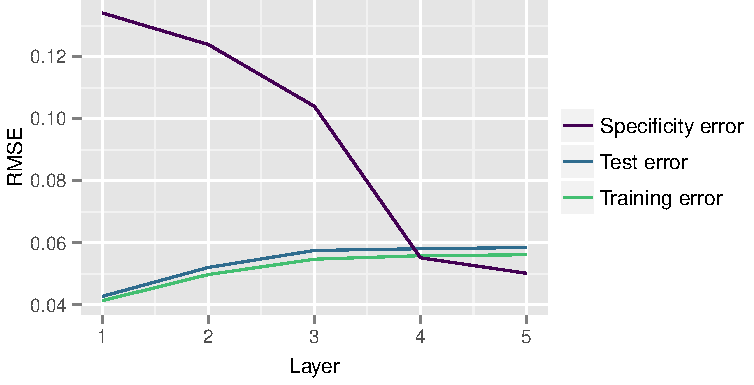
\includegraphics[width=0.8\textwidth]{figures/genspe}

\caption[Generalizability vs. specificity of a DBN for different numbers of
layers]{Generalizability vs. specificity of a DBN for different numbers of
layers. The similarity of the reconstruction errors between the training and
test images indicates that no overfitting occurs. The opposite slopes of the reconstruction errors and error of generated images (specificity error)
indicates a trade-off between generalizability vs. specificity in the earlier
phases of training, but the low errors at layer 5 indicate that the method is
both generalizable and specific.}
\label{fig:genspe}
\end{figure}

\begin{figure}[tb!]
\centering
% \includegraphics[width=0.5\textwidth, trim=0 0em 0 0]
%   {figures/MICCAI2013_sampled2d}
  
\begin{tikzpicture}
\tikzstyle{every node}+=[font=\small]
\node[inner sep=6pt] (manifold)
{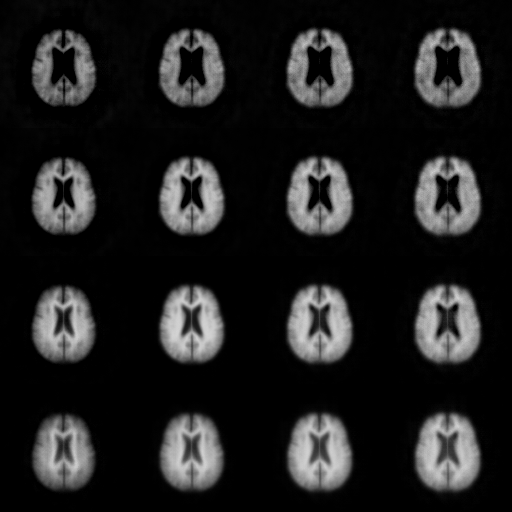
\includegraphics[width=0.5\textwidth]{figures/MICCAI2013_sampled2d}};

\draw[->] (manifold.south west)--node[below=5pt,inner sep=0] {$M_1$}
(manifold.south east);
\draw[->] (manifold.south west)--node[above=5pt,sloped,inner sep=0] {$M_2$}
(manifold.north west);

\end{tikzpicture}

\caption[Axial slices from generated volumes from the manifold]{Axial slices
from generated volumes from the manifold. An increase of the first and second manifold dimension visually correlates with an increase in
brain and ventricle size, respectively.}
\label{fig:generated}
\end{figure}

\subsubsection{Visualization of the Learned Manifold}

\ref{fig:generated} shows axial slices of 16 volumes sampled at the grid points
of a 2D regular grid in manifold space. Volumes sampled along the first manifold
dimension $M_1$ (from left to right) appear to increase in brain size, and the
images sampled along the second manifold dimension $M_2$ (from bottom to top)
appear to increase in ventricle size. \ref{fig:scatter} shows an axial slice of
each image of the training set plotted against its manifold coordinates.
Consistent with images sampled from the manifold, an increase in ventricle size,
which is indicative of brain atrophy (a hallmark of AD), visually correlates
with an increase of the second manifold coordinate. The AD/normal status is
indicated by the frame colour of each image. The vertical separation between AD
and normals suggests that the second manifold coordinate is potentially of
practical use in differentiating between AD and normal.

\begin{figure}[tb!] \centering
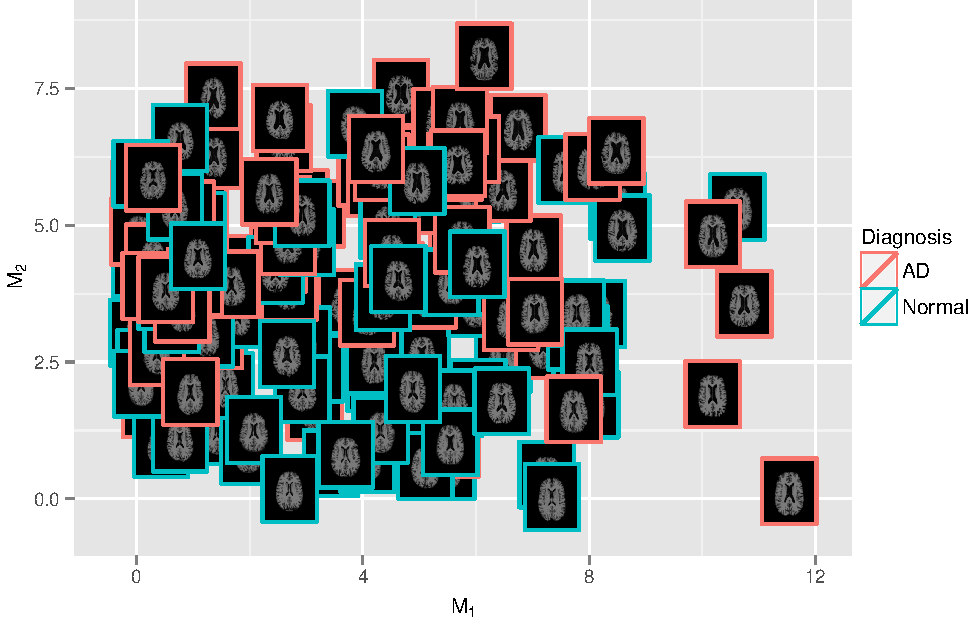
\includegraphics[width=\textwidth]{figures/scatterimage}
\caption[Axial slices of volumes from the training set plotted against their
manifold coordinates]{Axial slices of volumes from the training set plotted
against their manifold coordinates. The brains with larger ventricles, indicative of atrophy,
are mostly at the top, which is also where most of the AD patients are.}
\label{fig:scatter}
\end{figure}

\subsubsection{Correlations with Clinical Parameters}

To evaluate the potential of the manifold coordinates to reveal or predict
clinically relevant information, we have calculated the Pearson correlation $r$
of demographic parameters (age, gender) and disease parameters (MMSE score,
AD/normal status) with the manifold coordinates ($M_1$ and $M_2$). The results
of the correlation tests are summarized in \ref{tab:corr}. Age, MMSE and
AD/normal status show highly significant correlations with $M_2$ ($p$-values
between \num{9.85e-9} and \num{3.53e-7}), which makes intuitive sense because
$M_2$ visually correlates with ventricle size. The first manifold coordinate
correlates strongest with gender ($p\text{-value} = \num{8.24e-9}$), which also
makes sense in terms of the general difference in size between male and female.
The strength and significance of the correlations demonstrate the potential of
deep learning of brain images for classification and prediction of disease
status.

\begin{table}[tb]
\small
\centering
\caption[Pearson correlation of demographic and clinical parameters with
manifold coordinates]{Pearson correlation $r$ of demographic and
clinical parameters with manifold coordinates ($M_1$, $M_2$). The stronger
correlation in each column is highlighted in bold.}
\sisetup{
  round-mode = places,
  round-precision = 2,
  exponent-product = \cdot,
  detect-weight=true,detect-inline-weight=math,
  tight-spacing = true
}%

\begin{tabular}{l*{4}{@{\hspace{15pt}}cc}}
\toprule
& \multicolumn{2}{c}{Age} & \multicolumn{2}{c}{Gender} &
\multicolumn{2}{c}{MMSE} & \multicolumn{2}{c}{AD/Normal Status} \\
& $r$ & $p$-value & $r$ & $p$-value & $r$ & $p$-value
& $r$ & $p$-value \\
\midrule
% V1
$M_1$ &
\num{-0.1734} & \num{0.03378} &
\textbf{\num{0.4490381}} & \textbf{\num{8.239e-09}} &
\num{0.0116499} & \num{0.8875} &
\num{-0.03231144} & \num{0.6947} \\
% V2
$M_2$ &
\textbf{\num{0.4469}} & \textbf{\num{9.848e-09}} &
\num{0.1860143} & \num{0.02266} &
\textbf{\num{-0.4015518}} & \textbf{\num{3.527e-07}} &
\textbf{\num{0.4127084}} & \textbf{\num{1.536e-07}} \\
\bottomrule
\end{tabular}
\label{tab:corr}
\end{table}

\section[Variability of morphology and lesion distribution]{Variability of
Morphology and Lesion Distribution}

In this section, we present a new method for modelling the variability in brain
morphology and lesion distribution in a large set of MRIs of MS patients.
Similar to our previous work on modelling the manifold of brain MRIs of AD and
healthy subjects, our method is built using a DBN \citep{hinton2006b}, a layered
network whose parameters can be learned from training images. However, a
difference to the previous approach is that the DBN is trained on deformation
fields and lesions masks, instead of brain MRIs, in order to focus on the
learning of the variability in brain morphology and lesion distribution, without
the confounding influence of intensity variations. An advantage of DBNs over
other manifold learning methods is that it does not require a prebuilt proximity
graph, which is particularly beneficial for modelling lesions, because the
spareness and randomness of MS lesions make defining a suitable distance measure
challenging and potentially biasing. Instead, the DBN approach assumes that a
particular lesion configuration is a sample from an unknown distribution of
lesion configurations that can be parameterized by a relatively small set of
lesion distribution parameters. We model morphological and lesion variability
with two individual DBNs, then form a joint model by replacing the individual
top network layers with a new layer that joins both DBNs, similarly to the work
on the joint modelling of auditory and visual signals for speech recognition
\citep{ngiam2011}. Our results show that this model can automatically discover
the classic patterns of MS pathology, as well as more subtle ones, and that the
distribution parameters computed are found to have strong relationships to MS
clinical scores.

% Short overview. New data. Deformation fields directly and lesion masks for MS.
% Motivation for that: correspondence but without eliminating variability in
% morphology. Why use deep learning and not another method for that?

\subsection[Data sets and preprocessing]{Data Sets and Preprocessing}

The proposed method was evaluated on a data set from an MS clinical trial of 474
secondary progressive MS patients. For each subject, the data set contains one
\gls{t1w}, \gls{t2w}, and \gls{pdw} MRI with a resolution of \num{256x256x50}
voxels and a voxel size of \SI{0.937x0.937x3.000}{\milli\meter}. The main
preprocessing steps included rigid registration, brain extraction, intensity
normalization, and background cropping.

\begin{figure}[tb]
\centering
\begin{tikzpicture}[scale=0.75]
\tikzstyle{every node}=[font=\sffamily\small, inner sep=3pt, align=center]
\tikzstyle{every pin}=[align=center,fill=white]
\tikzstyle{dbnlabel}=[font=\sffamily]
         
% Deformation field
        
\node[dbnlabel, rotate=90] at (-1.5,2.25) {Morphology DBN};
        
\begin{scope}[xshift=-20pt,yslant=0.63,xscale=0.4]

\node[transform shape,pin={[pin
distance=8]125:Displacement\\
field $u$}] (field) at (2,2)
{\includegraphics[width=4cm]{figures/deformation2.png}};

% \node[pin={[pin distance=0.6,overlay]93:Displacement\\
% field $u$}] at ($(field.north west)!0.1!(field.north east)$) {};

\end{scope}
         
% 3-channel input

\foreach \x in {0, 10, 20} {
\begin{scope}[xshift=\x pt]
%\ifnum\x=0
%\path
%\else
\draw[fill=white, fill opacity=0.75]
%\fi
  (0,0) coordinate(A\x) -- ++(90:4) coordinate (B\x) -- ++(30:2) coordinate
  (C\x) -- ++(-90:4) -- cycle;
  

% \begin{scope}[xshift=-50pt,yslant=0.63,xscale=0.4]  
% \node[transform shape,inner sep=0pt] at (2,2)
%   {\includegraphics[width=4cm]{deformation2.png}};
% \end{scope}
  
\draw (0,3)
   ++(30:0.25) \ifnum\x=20 coordinate (a1) \else -- +(0:10pt) +(0:0) \fi
-- ++(90:0.5)  \ifnum\x=20 coordinate (b1) \else -- +(0:10pt) +(0:0) \fi
-- ++(30:0.25) \ifnum\x=20 coordinate (c1) \else -- +(0:10pt) +(0:0) \fi
-- ++(-90:0.5) \ifnum\x=20 coordinate (d1) \else -- +(0:10pt) +(0:0) \fi
-- ++(210:0.25);
\end{scope}
}

%\node[below=4pt,xshift=-3pt] at (A0)  {$u_x$};
%\node[below=4pt] at (A10) {$u_y$};
%\node[below=4pt,xshift=3pt] at (A20) {$u_z$};

\node[pin={[pin distance=5pt]260:$u_x$}] at (A0)  {};
\node[pin={[pin distance=5pt]270:$u_y$}] at (A10)  {};
\node[pin={[pin distance=5pt]290:$u_z$}] at (A20)  {};

% Transition

\draw ($(a1)!0.5!(c1)$) ++(55pt,-5pt) coordinate (e1);
\draw (a1) -- (e1);
\draw (b1) -- (e1);
\draw (c1) --node[pin={[pin distance=1cm]40:Strided\\ convolution}] {} (e1);
\draw (d1) -- (e1);

% First layer hidden units

\foreach \x in {80,85,90,95,100,105} {
\begin{scope}[xshift=\x pt,yshift=1.5cm,scale=0.5]
\draw[fill=white, fill opacity=0.75]
  (0,0) coordinate(A\x) -- ++(90:4) coordinate (B\x) -- ++(30:2) coordinate
  (C\x) -- ++(-90:4) coordinate(D\x) -- cycle;
   
\draw (0,2.5)
   ++(30:0.25) \ifnum\x=105 coordinate (a2) \else -- +(0:10pt) +(0:0) \fi
-- ++(90:1)    \ifnum\x=105 coordinate (b2) \else -- +(0:10pt) +(0:0) \fi
-- ++(30:0.5)  \ifnum\x=105 coordinate (c2) \else -- +(0:10pt) +(0:0) \fi
-- ++(-90:1)   \ifnum\x=105 coordinate (d2) \else -- +(0:10pt) +(0:0) \fi
-- ++(210:0.5);
\end{scope}
}

\draw[decorate,decoration={brace,raise=20pt}] (B0|-C0) --node[above=25pt]
{Strided convolutional RBM} (C105|-C0);

\draw[decorate,decoration={brace,raise=4pt,mirror}]
%(A80) --node[below=8pt] {$N = 32$} (A80-|D105);
(A80) --node[below=8pt] {$N = 32$} (A80-|D105);

\draw ($(a2)!0.5!(c2)$) ++(0:38pt) coordinate (e2);
\draw (a2) -- (e2);
\draw (b2) -- (e2);
\draw (c2) -- (e2);
\draw (d2) -- (e2);

% Second layer hidden units

\foreach \x in {145, 150, ..., 175, 180} {
\begin{scope}[xshift=\x pt,yshift=2.25cm,scale=0.25]
\draw[fill=white, fill opacity=0.75]
  (0,0) coordinate(A\x) -- ++(90:4) coordinate (B\x) -- ++(30:2) coordinate
  (C\x) -- ++(-90:4) coordinate(D\x) -- cycle;
\draw (0,1.75)
   ++(30:0.25) \ifnum\x=180 coordinate (a3) \else -- +(0:20pt) +(0:0) \fi
-- ++(90:2)    \ifnum\x=180 coordinate (b3) \else -- +(0:20pt) +(0:0) \fi
-- ++(30:1)    \ifnum\x=180 coordinate (c3) \else -- +(0:20pt) +(0:0) \fi
-- ++(-90:2)   \ifnum\x=180 coordinate (d3) \else -- +(0:20pt) +(0:0) \fi
-- ++(210:1);
\end{scope}
}

\draw[decorate,decoration={brace,raise=4pt,mirror}]
(A145) --node[below=8pt] {$N = 64$} (A145-|D180);

\draw ($(a3)!0.5!(c3)$) ++(0:18pt) coordinate (e3);
\draw (a3) -- (e3);
\draw (b3) -- (e3);
\draw (c3) -- (e3);
\draw (d3) -- (e3);

% Third layer hidden units

\foreach \x in {200, 205, ..., 240} {
\begin{scope}[xshift=\x pt,yshift=2.625cm,scale=0.125]
\draw[fill=white, fill opacity=0.75]
  (0,0) coordinate(A\x) -- ++(90:4) coordinate (B\x) -- ++(30:2) coordinate
  (C\x) -- ++(-90:4) coordinate(D\x) -- cycle;
\end{scope}
}

% Forth layer visible units (dense)

\begin{scope}[xshift=280pt, yshift=2.75cm]
\foreach \x/\y in {0/-2, 1/-1.5, 2/-1, 3/-0.5, 4/0, 5/0.5, 6/1, 7/1.5, 8/2} {
  \node[circle, draw] (v\x) at (0,\y) {};
}
\end{scope}

\draw[shorten >=10pt,shorten <=10pt,dashed] (A240)--(v0.south west);
\draw[shorten >=10pt,shorten <=10pt,dashed] (A240|-C240)--
node[label=120:Vectorize\\ hidden units] {} (v8.north west);

\draw[decorate,decoration={brace,raise=4pt,mirror}]
(A200) --node[below=8pt,fill=white] {$N = 32$} (A200-|D240);

%\node[rotate=90,fill=white,align=center] at(270pt,2.75cm) {Serialize\\ hidden
%units};

% Forth layer hidden units (dense)

\begin{scope}[xshift=320pt, yshift=2.75cm]
\foreach \x/\y in {0/-1, 1/-0.5, 2/0, 3/0.5, 4/1} {
  \node[circle, draw] (h\x) at (0,\y) {};
}
\end{scope}

\foreach \x in {0, ..., 8} {
  \foreach \y in {0, ..., 4} {
    \draw[very thin] (v\x)--(h\y);
  }
}

\draw[decorate,decoration={brace,raise=20pt}] (v8.west|-C0)
--node[above=25pt] {Dense RBM} (h0.east|-C0);

% Fifth layer hidden units (distribution parameters)

\begin{scope}[xshift=360pt, yshift=2.75cm]
\foreach \x/\y in {1/0.25, 2/-0.25} {
  \node[circle, draw, label=0:$D_\x$] (D\x) at (0,\y) {};
}
\end{scope}

\foreach \x in {0, ..., 4} {
  \foreach \y in {1,2} {
    \draw[very thin] (h\x)--(D\y);
  }
}

% \draw[decorate,decoration={brace,raise=22pt}]
% (D1.north-|D1.east) --node[above,sloped] {Deformation\\ parameters}
% (D2.south-|D2.east);

%%%%%%%%%%%%%%%%%%%%%
% Lesion Model
%%%%%%%%%%%%%%%%%%%%%

\begin{scope}[yshift=-6cm]

\node[dbnlabel, rotate=90] at (-1.5,2.25) {Lesion DBN};

\begin{scope}[xshift=-25pt,yslant=0.63,xscale=0.4] 
\node[transform shape,pin={[pin distance=15]140:Lesion\\
mask $l$}] at (2,2)
  {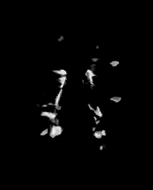
\includegraphics[height=4cm]{figures/lesions.png}};
\end{scope}

% 1-channel input

\foreach \x in {20} {
\begin{scope}[xshift=\x pt]
\draw[fill=white, fill opacity=0.75]
  (0,0) coordinate(A\x) -- ++(90:4) coordinate (B\x) -- ++(30:2) coordinate
  (C\x) -- ++(-90:4) coordinate (D\x) -- cycle;
  
\draw (0,3)
   ++(30:0.25) \ifnum\x=20 coordinate (a1) \else -- +(0:10pt) +(0:0) \fi
-- ++(90:0.5)  \ifnum\x=20 coordinate (b1) \else -- +(0:10pt) +(0:0) \fi
-- ++(30:0.25) \ifnum\x=20 coordinate (c1) \else -- +(0:10pt) +(0:0) \fi
-- ++(-90:0.5) \ifnum\x=20 coordinate (d1) \else -- +(0:10pt) +(0:0) \fi
-- ++(210:0.25);
\end{scope}
}

\node[pin=30:Visible\\ units] at ($(C20)!0.25!(D20)$) {};

% Transition

\draw ($(a1)!0.5!(c1)$) ++(55pt,-5pt) coordinate (e1);
\draw (a1) -- (e1);
\draw (b1) -- (e1);
\draw (c1) -- (e1);
\draw (d1) -- (e1);

% First layer hidden units

\foreach \x in {80,85,90,95,100,105} {
\begin{scope}[xshift=\x pt,yshift=1.5cm,scale=0.5]
\draw[fill=white, fill opacity=0.75]
  (0,0) coordinate(A\x) -- ++(90:4) coordinate (B\x) -- ++(30:2) coordinate
  (C\x) -- ++(-90:4) coordinate(D\x) -- cycle;
   
\draw (0,2.5)
   ++(30:0.25) \ifnum\x=105 coordinate (a2) \else -- +(0:10pt) +(0:0) \fi
-- ++(90:1)    \ifnum\x=105 coordinate (b2) \else -- +(0:10pt) +(0:0) \fi
-- ++(30:0.5)  \ifnum\x=105 coordinate (c2) \else -- +(0:10pt) +(0:0) \fi
-- ++(-90:1)   \ifnum\x=105 coordinate (d2) \else -- +(0:10pt) +(0:0) \fi
-- ++(210:0.5);
\end{scope}
}

\draw[decorate,decoration={brace,raise=4pt,mirror}]
%(A80) --node[below=8pt] {$N = 32$} (A80-|D105);
(A80) --node[below=8pt] {$N = 32$} (A80-|D105);

\draw ($(a2)!0.5!(c2)$) ++(0:38pt) coordinate (e2);
\draw (a2) -- (e2);
\draw (b2) -- (e2);
\draw (c2) -- (e2);
\draw (d2) -- (e2);

\node[pin=30:Hidden\\ units] at ($(C105)!0.2!(D105)$) {};

% Second layer hidden units

\foreach \x in {145, 150, ..., 175, 180} {
\begin{scope}[xshift=\x pt,yshift=2.25cm,scale=0.25]
\draw[fill=white, fill opacity=0.75]
  (0,0) coordinate(A\x) -- ++(90:4) coordinate (B\x) -- ++(30:2) coordinate
  (C\x) -- ++(-90:4) coordinate(D\x) -- cycle;
\draw (0,1.75)
   ++(30:0.25) \ifnum\x=180 coordinate (a3) \else -- +(0:20pt) +(0:0) \fi
-- ++(90:2)    \ifnum\x=180 coordinate (b3) \else -- +(0:20pt) +(0:0) \fi
-- ++(30:1)    \ifnum\x=180 coordinate (c3) \else -- +(0:20pt) +(0:0) \fi
-- ++(-90:2)   \ifnum\x=180 coordinate (d3) \else -- +(0:20pt) +(0:0) \fi
-- ++(210:1);
\end{scope}
}

\draw[decorate,decoration={brace,raise=4pt,mirror}]
(A145) --node[below=8pt] {$N = 64$} (A145-|D180);

\draw ($(a3)!0.5!(c3)$) ++(0:18pt) coordinate (e3);
\draw (a3) -- (e3);
\draw (b3) -- (e3);
\draw (c3) -- (e3);
\draw (d3) -- (e3);

% Third layer hidden units

\foreach \x in {200, 205, ..., 240} {
\begin{scope}[xshift=\x pt,yshift=2.625cm,scale=0.125]
\draw[fill=white, fill opacity=0.75]
  (0,0) coordinate(A\x) -- ++(90:4) coordinate (B\x) -- ++(30:2) coordinate
  (C\x) -- ++(-90:4) coordinate(D\x) -- cycle;
\end{scope}
}

%\node[rotate=90] at(270pt,2.75cm) {Serialize hidden units};

% Forth layer visible units (dense)

\begin{scope}[xshift=280pt, yshift=2.75cm]
\foreach \x/\y in {0/-2, 1/-1.5, 2/-1, 3/-0.5, 4/0, 5/0.5, 6/1, 7/1.5, 8/2} {
  \node[circle, draw] (V\x) at (0,\y) {};
}
\end{scope}

\draw[shorten >=10pt,shorten <=10pt,dashed] (A240)--(V0.south west);
\draw[shorten >=10pt,shorten <=10pt,dashed] (A240|-C240)--
%node[label=120:Vectorize\\ hidden units] {}
(V8.north west);

\draw[decorate,decoration={brace,raise=4pt,mirror}]
(A200) --node[below=8pt,fill=white] {$N = 32$} (A200-|D240);

%\node[rotate=90,fill=white,align=center] at(270pt,2.75cm) {Serialize\\ hidden
%units};

% Forth layer hidden units (dense)

\begin{scope}[xshift=320pt, yshift=2.75cm]
\foreach \x/\y in {0/-1, 1/-0.5, 2/0, 3/0.5, 4/1} {
  \node[circle, draw] (H\x) at (0,\y) {};
}
\end{scope}

\foreach \x in {0, ..., 8} {
  \foreach \y in {0, ..., 4} {
    \draw[very thin] (V\x)--(H\y);
  }
}

% Fifth layer hidden units (distribution parameters)

\begin{scope}[xshift=360pt, yshift=2.75cm]
\foreach \x/\y in {1/0.25, 2/-0.25} {
  \node[circle, draw, label=0:$L_\x$] (L\x) at (0,\y) {};
}
\end{scope}

\foreach \x in {0, ..., 4} {
  \foreach \y in {1,2} {
    \draw[very thin] (H\x)--(L\y);
  }
}
\end{scope}

%%%%%%%%%%%%%%
% Joint layer
%%%%%%%%%%%%%%

% yshift = 2.75 - 6/2 = -0.25

\begin{scope}[xshift=380pt, yshift=-0.25cm]
\foreach \x/\y in {1/-0.75, 2/-0.25, 3/0.25, 4/0.75} {
  \node[circle, draw, label=0:$J_\x$] (J\x) at (0,\y)
  {}; }
\end{scope}

\foreach \x in {0, ..., 4} {
  \foreach \y in {1, ..., 4} {
    \draw[very thin] (h\x)--(J\y);
    \draw[very thin] (H\x)--(J\y);
  }
}

\node[yshift=-15pt, fill=white, inner sep=3pt] at (h0) {$N = 16$};

\draw[decorate,decoration={brace,raise=30pt,mirror}] (V0.south-|J1)
--node[dbnlabel, below=35pt, sloped] {Joint DBN} (v8.north-|J1);

\end{tikzpicture}
\caption{DBN models used for discovering patterns.}
\label{fig:msdbnmodel}
\end{figure}

\subsection{Method}

\glsunset{icbm}\glsunset{mni}
Our proposed model for pattern discovery is illustrated in \ref{fig:msdbnmodel}
and consists of three main components (a) a model that aims to find patterns of
morphological changes in deformation fields (top pathway), (b) a model that aims
to find patterns in the spatial distribution of lesions (bottom pathway), and
(c) a joint model that aims to find concurring deformation and lesion
distribution patterns (combined pathways).

\subsubsection{Morphology Model}

The morphology model is learned from a set of displacement fields that are
calculated via non-rigid registration from a set of T1w brain MRIs $D \subset
I$, $I = \{I_n \mid I_n\colon\Omega \mapsto \R$\}, $\Omega \subset \R^3$ and the
\gls{icbm} 152 nonlinear atlas template image \citep{fonov2011}. First, all
images of the training set are aligned to \gls{mni} space by a 9
degree-of-freedom registration using the \gls{flirt} \citep{jenkinson2002}. Then
for each image $I_n \in D$, the displacement field $u_n$, $u\colon \Omega
\mapsto \R^3$, that describes the non-rigid transformation from template
coordinates to image coordinates is calculated using the \gls{fnirt}
\citep{andersson2007}, where the displacement field $u_n$ is represented by a
\num{40x48x22} grid of 3D displacement vectors. We assume that the displacement
fields $u_n$ are samples from an unknown distribution $p(u \mid D_1, \dotsc)$
that can be parameterized by far fewer parameters than the dimensionality of the
fields themselves. In practice, the user typically selects the number of
parameters to represent the data being explored. The task of finding patterns is
to discover the underlying probability density function $p(u \mid D_1, \dotsc)$,
where the parameters $(D_1,\dotsc)^T$ represent the patterns of variability of
the displacement field distribution. This allows us to compare the morphology of
two brains at a very high level in terms of the distribution parameters of their
displacement fields $u_1$ and $u_2$ given by $\E[D_1,\dotsc \mid u_1]$ and
$\E[D_1,\dotsc \mid u_2]$. Furthermore, we can visualize the modes of
morphological variability of MS brain images, by sampling the space of
displacement fields spanned by $(D_1, \dotsc)^T$ by calculating the expectation
$\E[u \mid D_1, \dotsc]$ for a range of values for $(D_1, \dotsc)^T$.

The probability density function $p(u)$ is modelled by a \gls{dbn}
\citep{hinton2006b}. The first RBM layer receives the displacement fields of a
training set as input and reduces the dimensionality of each field by
discovering patterns of similarity that are common within groups of displacement
fields. Each subsequent RBM receives the hidden unit activations of the previous
RBM as input, thus learning successively more complex and abstract patterns from
the training data. In particular, we use a DBN with three sconvRBMs and two
dense RBMs as described in \ref{sec:general_arch}. Compared to other more
commonly used convolution-based RBMs \citep{lee2009}, an advantage of sconvRBMs
is that inference is invertible, which allows the reconstruction of the visible
units from the hidden unit activations. In our application, this would allow for
the reconstruction of deformation fields from distribution parameters.

\begin{table}[t!]
\caption[Training parameters of the morphology DBN, lesion DBN, and joint
DBN]{Training parameters of the morphology DBN, lesion DBN, and joint DBN.
The visible units of the joint DBN are composed of the concatenated hidden
units of the first dense RBMs of the morphology and lesion DBNs.}
\label{tab:msdbn}
\centering
\small
\begin{tabular}{llccc}
\toprule
Layer & Parameter & Morphology DBN & Lesion DBN & Joint DBN \\
\midrule
Input     & Image size  & \num{40x48x22x3}  & \num{160x192x56x1} & --- \\
\addlinespace
sconvRBM1 & Stride size & \num{2x2x1}       & \num{4x4x2} & --- \\
          & Filter size & \num{10x10x7}     & \num{20x20x10} & --- \\
          & Filters     & 32                & 32 & --- \\
          & Output size & \num{16x20x16x32} & \num{36x44x24x32} & --- \\
\addlinespace
sconvRBM2 & Stride size & \num{2x2x2}       & \num{2x2x2} & --- \\
          & Filter size & \num{10x10x10}    & \num{14x14x10} & --- \\
          & Filters     & \num{64}          & \num{64} & --- \\
          & Output size & \num{4x6x4x64}    & \num{12x16x8x64} & --- \\
\addlinespace
sconvRBM3 & Stride size & \num{1x1x1}       & \num{2x2x2} & --- \\
          & Filter size & \num{3x5x3}       & \num{10x14x6} & --- \\
          & Filters     & 32                & 64 & --- \\
          & Output size & \num{2x2x2x32}    & \num{2x2x2x64} & --- \\
\addlinespace
RBM1      & Visible units & 256 & 512 & --- \\
          & Hidden units  &  16 & 16 & ---  \\
\addlinespace
RBM2      & Visible units & 16  & 16 & 32 \\
          & Hidden units  &  2  &  2 &  4 \\
\bottomrule
\end{tabular}
\end{table}

The parameters of the morphology DBN are summarized in \ref{tab:msdbn}. In
contrast to the DBN used to learn the manifold of brain MRIs of AD and healthy
subjects, we use valid convolutions for the sconvRBMs, because they allow a much
faster reduction of the dimensionality, especially for layers two and three,
where the image sizes are relatively small compared to the filter sizes. This
allows for a greater reduction of dimensionality within the sconvRBM layers, and
consequently for a more gradual reduction of the number of hidden units during
the transition of sconvRBMs to dense RBMs. To roughly compensate for the
anisotropic voxel size of the input images and corresponding deformation
fields, we chose an anisotropic filter and stride size of \num{10x10x7} and
\num{2x2x1}, respectively. After three sconvRBMs, the size of a deformation
field is reduced to \num{2x2x2x32} and small enough for RBMs.

Once the weights and bias terms of the DBN have been learned
from training data, we can use the model for inference. Let
$\vect{v}_{\text{d},1}, \dotsc, \vect{v}_{\text{d},5}$, $\vect{h}_{\text{d},1},
\dotsc, \vect{h}_{\text{d},5}$, and $\thetas_{\text{d},1}, \dotsc,
\thetas_{\text{d},5}$ denote the visible units, hidden units, and parameters,
respectively, of each RBM of the morphology DBN. Then, for a given displacement
field $u_n$, we can calculate the parameters $(D_1, \dotsc)^T$ of $u_n \sim p(u
\mid D_1, \dotsc)$ with
\begin{align} 
(D_1, \dotsc)^T &= \E[D_1, \dotsc \mid u_n] = \E[\vect{h} \mid
\vect{v}_{\text{d},5}, \thetas_{\text{d},5}] \\
\vect{v}_{\text{d},i+1} &= \E[\vect{h} \mid \vect{v}_{\text{d},i},
\thetas_{\text{d},i}]
\end{align}
where $i \in [1,4]$ and $\vect{v}_{\text{d},1} = u_n$. Inversely, the mean
displacement field $\bar{u}$ given the distribution parameters can be calculated
by
\begin{align}
\bar{u} &= \E[u \mid D_1, \dotsc] = \E[\vect{v} \mid \vect{h}_{\text{d},1},
\thetas_{\text{d},1}] \\
\vect{h}_{\text{d},i} &= \E[\vect{v} \mid \vect{h}_{\text{d},i+1},
\thetas_{\text{d},i+1}]
\end{align}
where $i \in [1,4]$ and $\vect{h}_{\text{d},5} = (D_1,\dotsc)^T$.

\subsubsection{Lesion Model}

The input into our lesion model is a set of 3D binary lesion masks $l_n \in I$,
which have been created from T2w and PDw MRIs by experts using a semi-automatic
method. All lesion masks are spatially aligned to MNI space using the
transformations as calculated for the corresponding T1w images. Analogous to the
morphology model, we assume that lesion masks $l_n$ are samples from an unknown
distribution $l_n \sim p(l \mid L_1, \dotsc)$ that can be parameterized by only
relatively few parameters $(L_1, \dotsc)^T$. The task of finding lesion patterns
is to discover the underlying probability density function $p(l \mid L_1,
\dotsc)$, where the parameters $(L_1, \dotsc)^T$ represent patterns of
variability of MS lesions. Similar to the morphology DBN, the lesion DBN
consists of three sconvRBMs and two dense RBMs, whose parameters are summarized
in \ref{tab:msdbn}. For the first layer, we chose an anisotropic stride size of
\num{4x4x2}, to roughly compensate for the anisotropic voxel size of the input
images. A limiting factor for the choice of parameters is the amount of
available GPU memory. Due to the much higher resolution of the lesion masks
compared to the deformation fields, we increased the stride size compared to the
morphology DBN in order to reduce the required amount of memory for storing the
hidden units of the first layer and visible units of the second layer. Choosing
a stride size of \num{4x4x2} reduces the size of one channel by a factor of
roughly 32, which allows the use of 32 filters, while keeping the amount of
memory required to train the second layer roughly equal compared to the first
layer. To account for the sparse activation of MS lesion masks, we constrain the
filter learning process to a pre-defined ROI, which was chosen to contain all
white matter lesions from the training set. Similarly to the morphology model,
for a trained lesion DBN and a given lesion mask $l_n$, we can calculate the
parameters $(L_1,\dotsc)^T$ of $l_n \sim p(l\mid L_1,\dotsc)$ by
\begin{align} 
(L_1, \dotsc)^T &= \E[L_1, \dotsc \mid l_n] = \E[\vect{h} \mid
\vect{v}_{\text{l},5}, \thetas_{\text{l},5}] \\
\vect{v}_{\text{l},i+1} &= \E[\vect{h} \mid \vect{v}_{\text{l},i},
\thetas_{\text{l},i}]
\end{align}
where $i \in [1,4]$ and $\vect{v}_{\text{l},1} = l_n$. Likewise, the mean lesion
configuration $\bar{l}$ given the distribution parameters $(L_1,\dotsc)^T$ can
be calculated by
\begin{align}
\bar{l} &= \E[l \mid L_1, \dotsc] = \E[\vect{v} \mid \vect{h}_{\text{l},1},
\thetas_{\text{l},1}] \\
\vect{h}_{\text{l},i} &= \E[\vect{v} \mid \vect{h}_{\text{l},i+1},
\thetas_{\text{l},i+1}]
\end{align}
where $\vect{v}_{\text{l},1}, \dotsc, \vect{v}_{\text{l},5}$,
$\vect{h}_{\text{l},1}, \dotsc, \vect{h}_{\text{l},5}$, and
$\thetas_{\text{l},1}, \dotsc, \thetas_{\text{l},5}$ denote the visible units,
hidden units, and parameters of each RBM of the lesion DBN, respectively, $i \in
[1,4]$, and $\vect{h}_{\text{l},5} = (L_1,\dotsc)^T$.

\subsubsection{Joint Model}

To discover concurring patterns of morphology and lesion distribution, we
combine the morphology DBN and the lesion DBN to form the joint DBN, which
defines the joint distribution $p(u, l \mid J_1, \dotsc)$. The joint DBN
consists of two pathways (see \ref{fig:msdbnmodel}), each corresponding to the
first 4 layers of the morphology and lesion DBNs, respectively, and a 5th RBM
layer with 4 hidden units, which replaces the 5th layer of the individual DBNs
and combines the hidden unit activations of the 4th layer RBMs. That is, the 5th
RBM defines the joint probability $p(\vect{v}_\text{j}, \vect{h}_\text{j} \mid
\thetas_\text{j})$, where the vector $\vect{v}_\text{j}$ contains the
concatenated hidden units of the 4th layer RBMs, $\vect{v}_\text{j} =
(\vect{h}_{\text{d},4}^T, \vect{h}_{\text{l},4}^T)^T$, and $\vect{h}_\text{j} =
(J_1, \dotsc)^T$ are the modes of variability of morphological and lesion
distribution changes.

\subsection{Results}

\subsubsection[Visualization of patterns of variability]{Visualization of
Patterns of Variability}

The invertibility of our model allows the reconstruction of images from the
distribution parameters to visualize the discovered patterns of variability.
\ref{fig:samples}\subref{fig:deformations} shows axial slices from volumes
generated from the 2-parameter morphology model $p(u \mid D_1, D_2)$. To
generate these images, we calculated the mean displacement fields for varying
values of $D_1$ and $D_2$ to span the range of variability represented by the
training set and applied the inverse deformations to the ICBM 152 template
image. The most apparent morphological variability captured by the morphology
model is ventricular enlargement for $D_1$ and overall brain size for $D_2$.
\ref{fig:samples}\subref{fig:lesions} shows axial slices from the mean lesion
configurations $\E[l \mid L_1, L_2]$ for varying lesion distribution parameters.
An increase of $L_2$ visually correlates with an increase of lesions
specifically around the ventricles, whereas an increase of $L_1$ visually
correlates with an increase of lesions in the entire white matter.

\begin{figure}[tb]
\newlength{\subfigwidth}
\setlength{\subfigwidth}{0.27\textwidth}
\centering
\subfloat[Morphology manifold] {
\label{fig:deformations}
\begin{tikzpicture}
\tikzstyle{every node}+=[font=\small]
\node
(manifold){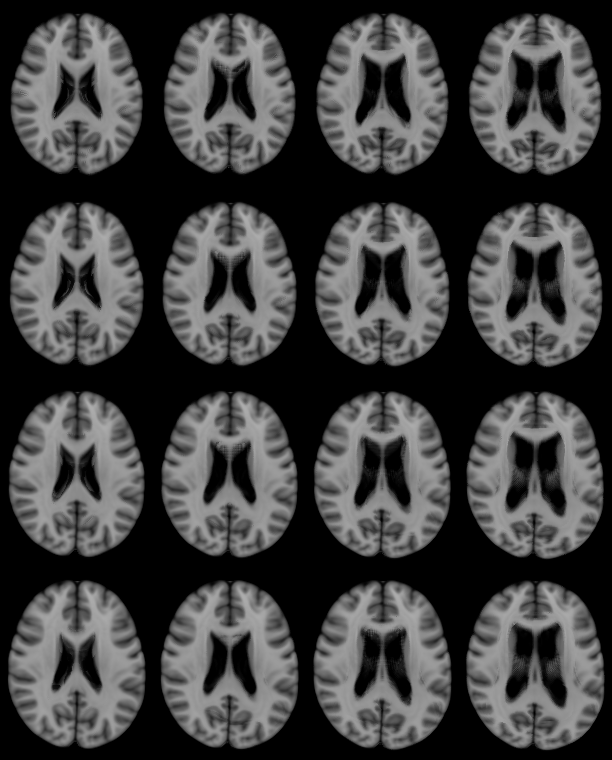
\includegraphics[width=\subfigwidth]{figures/MICCAI2014_warps_t1_dark}};

\draw[->] (manifold.south west)--node[below=5pt,inner sep=0] {$D_1$}
(manifold.south east);
\draw[->] (manifold.south west)--node[above=5pt,sloped,inner sep=0] {$D_2$}
(manifold.north west);

\end{tikzpicture}
}
\subfloat[Lesion manifold] {
\label{fig:lesions}
\begin{tikzpicture}
\tikzstyle{every node}+=[font=\small]
\node
(manifold){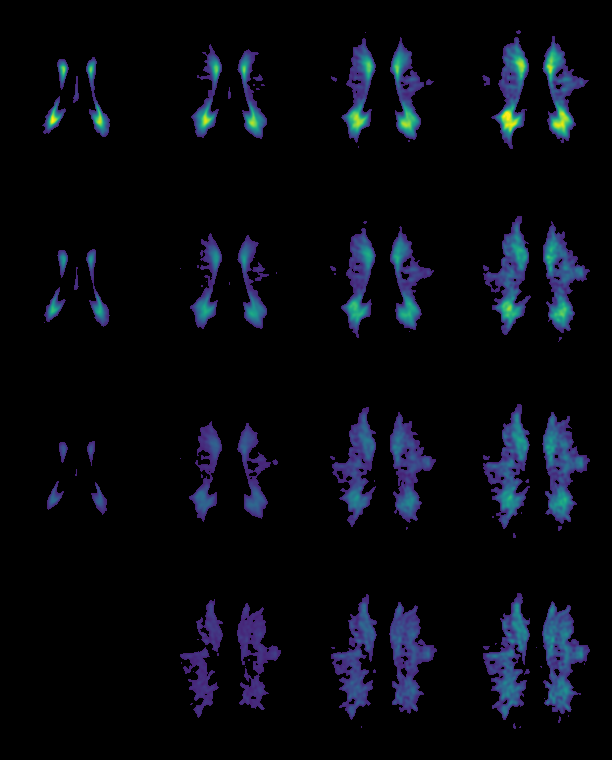
\includegraphics[width=\subfigwidth]{figures/MICCAI2014_viridis_p442_d0_full_h16-2}};

\draw[->] (manifold.south west)--node[below=5pt,inner sep=0] {$L_1$}
(manifold.south east);
\draw[->] (manifold.south west)--node[above=5pt,sloped,inner sep=0] {$L_2$}
(manifold.north west);

\end{tikzpicture}
}%
\subfloat[Joint manifold] {
\label{fig:joint}
\begin{tikzpicture}
\tikzstyle{every node}+=[font=\small]

\node[align=left,fill=black,inner sep = 0pt] (manifold1) {
  \mbox{}\\[2pt]
  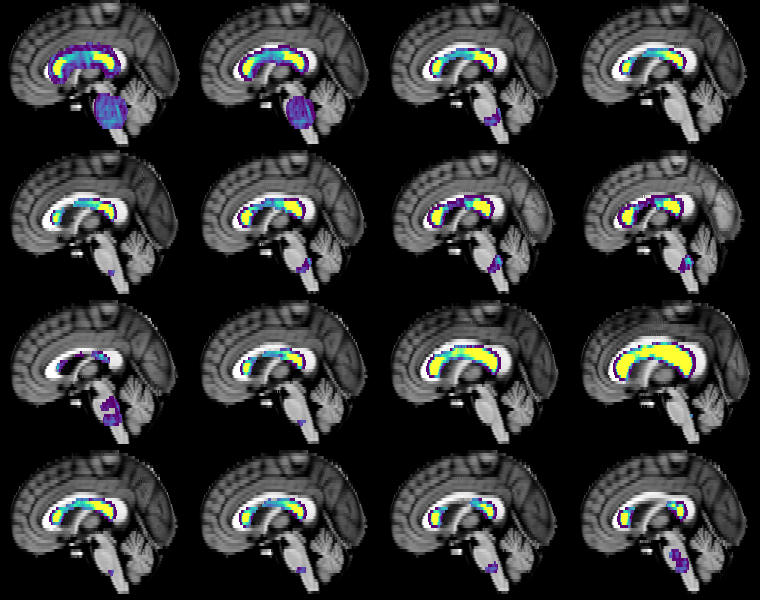
\includegraphics[trim=0 340 0 0,clip,width=\subfigwidth]
    {figures/MICCAI2014_viridis_full_rl1_h4_sag}\\[8.5pt]
  \includegraphics[trim=0 0 0 150,clip,width=\subfigwidth]
    {figures/MICCAI2014_viridis_full_rl1_h4}
};
\node[fit=(manifold1)] (manifold) { };

\foreach \x/\y in {0.125/1, 0.375/2, 0.625/3, 0.875/4} {
  \node[left=1pt,inner sep=0pt] at ($(manifold.north west)!\x!(manifold.south
  west)$) {$J_\y$}; }

\draw[->] (manifold.south west)--node[below=5pt,inner sep=0] {$J_x$}
(manifold.south east);

\end{tikzpicture}
} \caption[Slices from generated volumes from the morphology, lesion,
and joint model]{Slices from generated volumes from the (a) morphology, (b)
lesion, and (c) joint model. The morphology model captures ventricular
enlargement ($D_1$) and decrease in brain size ($D_2$) as the main modes of
variation. For the lesion model, $L_1$ captures an increase in lesion load
throughout the WM, while $L_2$ captures primarily periventricular lesion load
variations. The parameters of the joint model capture combinations
of the variability found in the individual models.}
\label{fig:samples}
\end{figure}

To visualize concurring patterns of morphology and lesion distribution, we
sampled images from the joint model $p(u, l \mid J_1, \dotsc, J_4)$ as shown in
\ref{fig:samples}\subref{fig:joint}. The images are deformed template images
with superimposed lesion masks. For each row, we varied only one distribution
parameter and set the remaining parameters to their mean values. Of the four
parameters, $J_3$ visually corresponds most closely to the ``classic''
progression of MS pathology, with an enlargement of the ventricles paired with
an increased periventricular lesion load. The parameters $J_2$ and $J_4$ also
reveal simultaneous morphological and lesion variations that are visible on the
chosen axial slice. For $J_1$, a lesion pattern is not obvious unless the images
are viewed sagittally, which reveals changes in lesion load in the pons.

\subsubsection{Correlations with Clinical Scores}

\begin{table}[tb]
\centering 
%\small

\caption[Pearson correlations of clinical scores with distribution parameters
and imaging biomarkers]{Pearson correlations $r$ of clinical scores with
distribution parameters of the morphology model ($D_1$, $D_2$), lesion model ($L_1$, $L_2$), joint model ($J_1$, $J_2$, $J_3$, $J_4$), normalized brain volume (nBV), and
lesion load (LL). The level of statistical significance is indicated by the
number of asterisks (* $p < 0.05$, ** $p < 0.01$, *** $p < 0.001$).
}

%\NewDocumentCommand{\sym}{m}{#1}

\label{tab:correlations}
\sisetup{
  round-mode = places,
  round-precision = 3,
  exponent-product = \cdot,
  detect-weight=true,
  detect-inline-weight=math,
  tight-spacing = false,
  table-align-text-post = false
}%

\def\tabspace{14pt}

\begin{tabular}{c@{\hspace{\tabspace}}c%
@{\hspace{\tabspace}}S[table-format=2.5]%
@{\hspace{\tabspace}}S[table-format=2.6]
@{\hspace{\tabspace}}S[table-format=2.6]
@{\hspace{\tabspace}}S[table-format=2.6]}
\toprule
 &  & {T25W} & {9-HPT} & {PASAT} & {MSFC} \\
 \midrule
 
\multirow{4}*{\minitab[c]{Individual\\ models}}
 & $D_1$ &
\bfseries -0.128976787246536** & -0.214588136146619*** & -0.282044527648157*** &
-0.314633263656368*** \\
 & $D_2$ & 0.0870255979372807 & 0.115835195120173* & 0.08923208653141 &
0.138616500875685** \\
& $L_1$ & -0.0581629511079419 & -0.231012897586838*** & -0.391822792658197*** &
-0.366992537420278*** \\
& $L_2$ & -0.091057480388512 & \bfseries -0.354478789398171*** &
\bfseries -0.426543205964196*** & \bfseries -0.463860459137063*** \\
\addlinespace
\multirow{4}*{\minitab[c]{Joint\\ model}}
 & $J_1$ & 0.107219513748914* & 0.285812780188632*** & 0.336253511146623*** &
0.378889115681159*** \\
 & $J_2$ & -0.037731447660239 & -0.209982769437628*** & -0.226800472678912***
& -0.255585426983655*** \\
& $J_3$ & \bfseries -0.117780586822506* & \bfseries -0.369169927947271*** &
\bfseries -0.452556545437486*** & \bfseries -0.494130959187706*** \\
& $J_4$ & -0.0491209563011896 & -0.205764640863705*** & -0.382954826511733*** &
-0.345529171963859*** \\
\addlinespace
\multirow{2}*{\minitab[c]{Imaging\\ biomarkers}}
 & nBV & 0.0530068558456253 & 0.143905618421747** & 0.246833144651129***
& 0.234774254053599*** \\
 & LL & -0.073681606595365 & \bfseries -0.286360084620956*** &
\bfseries -0.399646128024074*** & \bfseries -0.406222020153583*** \\
  
 \bottomrule
\end{tabular}

\end{table}

\glsunset{t25w}\glsunset{x9pt}\glsunset{pasat}\glsunset{nbv}\glsunset{ll}
To evaluate the potential of the distribution parameters to reveal clinically
relevant information, we have calculated the Pearson correlation $r$ of the
clinical MS Functional Composite (MSFC) score \citep{fischer1999} and its
components (\glslink{t25w}{Timed 25-Foot Walk, T25W}; \glslink{x9pt}{9-Hole Peg
Test, 9-HPT}; \glslink{pasat}{Paced Auditory Serial Addition Test, PASAT}) with
the distribution parameters and two established MS imaging biomarkers
(\glslink{nbv}{normalized brain volume, nBV}, as calculated by SIENAX
\citep{smith2002} and \glslink{ll}{lesion load, LL}). The results of the
correlation tests are summarized in \ref{tab:correlations}. In the individual
models, all parameters correlate significantly with 9-HPT, PASAT, and MSFC,
except for $D_2$, which did not show a statically significant correlation with
PASAT. The morphology parameter $D_1$ correlates more strongly with these scores
than nBV, as does the lesion parameter $L_2$ than LL. For T25W, $D_1$ shows a
modest but significant correlation while nBV does not. In the joint model, all
parameters correlate significantly with 9-HPT, PASAT, and MSFC, with $J_3$ being
particularly strong. The parameter $J_3$ shows stronger correlations than nBV or
LL for all clinical scores, including a modest significant correlation to T25W,
which is not shown by nBV nor LL. The significant correlation between $J_1$ and
T25W is particularly interesting because the lesion changes modelled by $J_1$
occur in the pons, which is known to be of clinical significance for mobility.
Overall, the learned parameters correlate better than the established imaging
biomarkers.

\begin{figure}[tb]
\centering
\subfloat[Morphological changes] {
\begin{tikzpicture} 
\tikzstyle{every node}=[font=\scriptsize]
\node[align=left,inner sep=0] (images) {
\includegraphics[width=0.47\textwidth]{figures/MICCAI2014_full_rl1_h4_MSFC_nolesion}
\\
\includegraphics[width=0.47\textwidth]{figures/MICCAI2014_full_rl1_h4_MSFC_sag_nolesion}
};
\foreach \x/\y in {0.1/1.5, 0.3/0, 0.5/-1.5, 0.7/-3, 0.9/-4.5} {
  \node[above=2pt] at ($(images.north west)!\x!(images.north east)$) {$\y$}; }
\end{tikzpicture}
}
\subfloat[Lesion changes] {
\begin{tikzpicture}
\tikzstyle{every node}=[font=\scriptsize] 
\node[align=left,inner sep=0] (images) {
\includegraphics[width=0.47\textwidth]{figures/MICCAI2014_viridis_full_rl1_h4_MSFC}
\\
\includegraphics[width=0.47\textwidth]{figures/MICCAI2014_viridis_full_rl1_h4_MSFC_sag}
};
\foreach \x/\y in {0.1/1.5, 0.3/0, 0.5/-1.5, 0.7/-3, 0.9/-4.5} {
  \node[above=2pt] at ($(images.north west)!\x!(images.north east)$) {$\y$};
}
\end{tikzpicture}
}
\caption[Axial and mid-sagittal slices of volumes representing the spectrum of
MSFC scores]{Axial (top row) and mid-sagittal (bottom row) slices of volumes
representing the spectrum of MSFC scores from \num{1.5} to \num{-4.5}. A
decrease in MSFC shows the classic pattern of MS pathology.}
\label{fig:msspectrum}
\end{figure}

\subsubsection{Progression of a ``Mean'' SPMS Brain along a Range of MSFC
Scores}

Another benefit of our model is the ability to visualize the progression of a
``mean'' \gls{spms} brain along a range of MSFC scores.
To demonstrate, we trained four independent linear models to predict the
distribution parameters $J_1, \dotsc, J_4$ given the MSFC ($J_i = a_i +
b_i\text{MSFC}$). \ref{fig:msspectrum} shows the axial (top row) and
mid-sagittal (bottom row) slices of generated images representing the range of
MSFC scores from \num{1.5} to \num{-4.5}. Consistent with previous results, a
decrease in MSFC visually correlates with an increase in the size of the
ventricles, an increase in periventricular lesions, and an increase in lesions
in the pons region.

\section{Summary}

% We have proposed a novel approach to learning the manifold of brain MRIs. In
% contrast to previous work, our approach does not require an explicitly defined
% similarity measure, or building a proximity graph. Furthermore, we have shown
% that the learned manifold coordinates capture shape variations of the brain that
% correlate with demographic and disease parameters. Our manifold learning method
% uses deep learning to discover patterns of similarity and variability within a
% group of images. Our proposed DBN training algorithm is much more efficient than
% traditional, convolution-based methods and, when parallelized on graphics
% processors, makes DBN training on 3D MRIs practical for the first time. For
% future work, we plan to incorporate clinical parameters into the training
% process to learn a model of the joint probability of images and associated
% clinical parameters. We would also like to investigate the effect of spatial
% normalization using affine or deformable registration, which we expect would
% result in further improvements in correlations with clinically relevant
% parameters. In addition, we would like to compare our method to other
% state-of-the-art brain manifold learning methods to investigate relative
% strengths and weaknesses for particular clinical applications such as the
% prediction of mild cognitive impairment to AD conversion, which is a topic of
% strong clinical interest.

We have introduced a new method for modelling the variability in brain morphology
and lesion distribution of a large set of MRIs of AD and MS patients. We have
proposed two models, both of which are based on DBNs. In our first approach,
variability of brain morphology is modelled as a manifold of brain MRIs. In our
second approach, we train three DBNs: one for morphology, one for lesion
distribution, and one that jointly models both. The morphology model is learned
from deformation fields, which allows the algorithm to focus on structural
changes without the confound of contrast variations between images. We have
demonstrated that such a model, which requires no built-in priors on image
similarity, can automatically discover patterns of variability that can be
parameterized in a low-dimensional space and are clinically relevant. In
addition, our model can generate sample images from model parameters for
visualization. 

%In addition, we would like to extend our approach to model longitudinal
% patterns of variability with the goal of predicting future clinical status from current
%images.

\chapter{Conclusions and Future Work}
\label{sec:conclusions}

In this thesis, we have addressed two challenges for measuring the state and
progression of \gls{ms}. In \ref{sec:segmentation}, we presented a fully
automatic segmentation method of MS lesions, which enables the accurate
computation of lesion-based imaging biomarkers such as lesion load and lesion
count. In \ref{sec:manifold}, we presented a novel method for the automatic
discovery of patterns of variability in MS subjects that show improved
correlations to clinical scores over traditional volumetric biomarkers. Both
methods are based on deep learning, a class of algorithms that can learn a
feature hierarchy from a set of images. A major challenge of deep learning
methods is the time and memory required to process large 3D volumes. To address
this challenge, we have developed a novel training algorithm for convolutional
deep learning methods that facilitates the training of full resolution 3D
medical images and presented our algorithm with a comprehensive comparison with
alternative training methods in \ref{sec:training}. Although the developed
methods were developed and evaluated in the context of MS, the methods are very
general and can potentially be applied to various segmentation and manifold
learning problems.

\section{Contributions}

In the course of developing deep learning-based methods for MS lesion
segmentation and pattern discovery, we have made the following contributions:
\begin{itemize}
\item We have developed a novel training algorithm for \glspl{cdbn} and
\glspl{cnn} that performs training in the frequency domain. The speed-ups gained
by our method compared to spatial domain implementations and the reduced memory
requirements compared to other frequency domain methods facilitate the
application of deep learning to high-resolution 3D medical images.
  
\item We have developed a neural network architecture that jointly learns the
features required to segment MS lesions and to perform the segmentation based on
the automatically learned features. The joint learning of feature extractor and
classifier facilitates the learning of features that are robust to the
variability of MS lesions and varying contrasts produced by different scanners.

\item We have developed a novel objective function for training neural networks
that is suitable for the classification of vastly unbalanced classes, such as
the segmentation of MS lesions, which typically comprise less than one percent
of the image.

\item We have demonstrated that the use of shortcut connections in the proposed
neural network architecture allows for the learning of features at different
scales, which facilitates the segmentation of both very small and very large
lesions.

\item We have developed a framework for modelling changes in brain morphology
and lesion distribution with only a few parameters, which also show improved
correlation with clinical scores compared to established volumetric imaging
biomarkers. In contrast to previous manifold learning approaches, our method
does not assume that the ambient space is locally linear and also does not
require the definition of a suitable similarity measure, or building a proximity
graph.
\end{itemize}

\section[Future work]{Future Work}

\subsection[New applications of deep learning]{New Applications of Deep
Learning}

Motivated by the success of deep learning for the two applications explored in
this theses, a possible direction for further research is to investigate new
applications of deep learning. The success of deep learning methods mostly stems
from their ability to learn feature hierarchies directly from the data. This
allows deep learning methods to adapt to the challenges presented by the data,
such as imaging artifacts and contrast variations, without explicitly having to
model them. However, deep learning methods can take a lot of time to train and
require large amounts of training data in order to learn a feature
representation that generalizes well to new data samples. To overcome those
challenges, first applications of deep learning were limited to problems that
can be cast as a patch-wise classification problem, such as the segmentation of
cell membranes \citep{ciresan2012} and the detection of cell carcinoma
\citep{cruz2013}. In this fashion, every patch of an image is considered a
training sample, which greatly increases the amount of labelled training cases.
In addition, training on relatively small 2D patches made training feasible.
Similarly, fully convolutional approach for image segmentation leverage every
pixel of an image as a training sample, while being more computationally
efficient than patch-based approaches. However, layers deeper in the hierarchy
have increasingly fewer pixels, and are consequently trained with fewer training
samples, which increases the risk of overfitting.

An interesting research question is therefore what other problems can be solved
using deep learning. The proposed segmentation framework can readily be applied
to various segmentation problems. Preliminary results on the segmentation of the
corpus callosum show great promise. For future work, it will be important to
explore other segmentation problems. Another potential application could be the
detection of landmark points. Detecting landmarks is similar to segmentation in
that every voxel of an image can be leveraged as a training sample. However, the
number of positive samples per image is much lower than for segmentation, which
might require further research. A potential solution to deal with the sparseness
of a landmark map is to train the model on a distance transformation of the
original landmark map.

A different stream of potential applications is to incorporate deep learning
into existing model learning frameworks. Originally, active shape
\citep{cootes1995} and active appearance \citep{cootes2001} models employ
principal component analysis in order to reduce the dimensionality of the input
feature space. Similarly, deep belief networks or stacked autoencoders can be
used for dimensionality reduction, which might yield to the learning of more
biologically plausible models, due to their ability to find highly nonlinear
patterns of variability in the data.

\subsection[Improving the performance on small data sets using data
augmentation]{Improving the Performance on Small Data Sets using Data
Augmentation}

A promising approach of improving the performance on small data sets is data
augmentation. Data augmentation allows the artificial increase of the training
data set size by generating new training samples from existing ones. Data
augmentation has been successfully used to deal with the problem of small
medical data sets. For example, \citet{ronneberger2015} used automatically
generated deformations to artificially increase the data set size for segmenting
cells, but also simpler data augmentation techniques such as adding rotations,
translations and contrast variations can help to avoid overfitting. However,
hand-engineered data augmentation approaches depend on how well the variability
in the data is understood. Alternatively, automatically learned unsupervised
deep generative models such as deep belief networks can potentially be used to
learn the variability of the training data in order to generate new samples that
are biologically plausible.

\subsection[Rotation-invariant neural networks]{Rotation-invariant Neural
Networks}

Although neural networks are able to learn features that are invariant to the
variability in the data, doing so often requires the learning of different
variants of the same feature in order to capture the range of variability. In
order to decrease the number of weights of a neural network, and therefore to
reduce the training time and risk of overfitting, different neural network
architectures have been developed with build-in invariance or equivariance
properties. For example, previously used sigmoid activation functions are
sensitive to the intensity range of the input, which requires the relearning of
feature detectors for images with varying contrast. To overcome, rectified
linear units were proposed, which represent the same units with different
biases, which makes them equivariant to intensity variations. In order to allow
the learning of translational invariant features, convolutional neural networks
were developed, which greatly reduce the number of weights required to capture
simple edge detecting features at different locations in the image compared to
dense neural networks. However, features learned by a convolutional neural
network are not invariant to rotations. This leads, for example, to the learning
of a variety of edge detecting features that are sensitive to different angles.
While the number of angles is rather low in 2D, significantly more features are
required to span the space of rotations in 3D, due to the combination of three
rotation parameters. In order to avoid the learning of very basic features with
different rotation parameters in 3D, it might therefore be necessary to develop
neural network architectures that are inherently invariant or equivariant to
rotations, which would allow for the learning of a diverse set of features that
capture fine details in 3D with much fewer weights than currently employed
convolutional neural network architectures.

\subsection[Increasing the expressive power of single neurons]{Increasing the
Expressive Power of Single Neurons}

Current neural networks can only calculate the weighted sum of its inputs
followed by the application of a nonlinear function. Although it has been shown
that this model is able to approximate any function, doing so might require a
lot of units and layers, which makes them harder to train and requires more
training data in order to reduce the risk of overfitting. One way to increase
the expressive power of neural networks without increasing their complexity is
to design more computationally powerful units. In their review of the
computational properties of dendrites, \citet{london2005} noted that some
neurons were found that are able to calculate the multiplication of its inputs.
For example, the looming sensitive neurons in the locust's visual system are
able to detect approaching objects on a collision course by calculating the
multiplication of angular size and speed of approaching object. The
multiplication is possible encoded as the sum of logarithmic inputs followed by
exponentiation. Similarly, \citet{godfrey2016} have proposed a type of neuron
for artificial neural networks that is able to learn to calculate the logarithm
or exponential of its inputs, which allows for the learning of networks that can
calculate arbitrary polynomial with significantly fewer parameters than
traditional ReLU or sigmoid neural networks. Alternatively, \citet{livni2013}
have proposed a network architecture that can learn arbitrary polynomials using
a combination of units that calculate weighted sums of an arbitrary number of
inputs and units that calculate the product of two inputs. However, these
network architectures needs to be investigated further in order to show if the
theoretical advantages translate into improvements on practical problems.


\singlespacing
% \nocite{*}
\bibliography{bibliography/newestbib}

%\appendix

%\include{chapters/A_gpudetails}

\end{document}

%\chapter{Discussion}

What else do I need? General discussion of the role of deep learning for medical
image analysis. Maybe.

Role of deep learning for medical imaging

advantages: fewer assumptions (manifold learning), generally applicable, learns
variability, less human supervision (segmentation), end-to-end-learning. Quick
adaption to new problems.

Challenges: large amounts of training data, how to get more labels? Data
augmentation. How to deal with large amounts of data? Scalability. Tasks deep
learning can be good at? Tedious and well defined tasks for which training data
is available, identifying landmarks, segmentation, classification of voxels for,
e.g., cancer cell detection. Why? Because a single image can provide a lot of
data. For per-image deep learning need a lot of data. Finding patterns in
images, diagnosis. Current models not sensitive enough, but if more sensitive,
they might over fit.

%\chapter{Future Work}

Future work: different models like RNNs, LSTMs. Learning
invariance to rotations might help especially in 3D. What are other
applications? Also need to understand models better. Visualize them maybe?
Better training algorithms? More data? Better regularization?
